\documentclass[a4paper,11pt]{article}
%%\documentclass[a4paper,12pt]{amsart}
\usepackage[cp1252]{inputenc}
\usepackage[spanish]{babel}
\usepackage{amsmath}
\usepackage{amsthm}
\usepackage{amssymb}
\usepackage{amsfonts}
\usepackage{graphicx}
\usepackage{cancel}
\usepackage{color}
\usepackage{multirow}
\usepackage{colortbl}
\usepackage{enumerate}

\setlength{\textheight}{23.5cm} \setlength{\evensidemargin}{0cm}
\setlength{\oddsidemargin}{-0.8cm} \setlength{\topmargin}{-2.5cm}
\setlength{\textwidth}{17.5cm} \setlength{\parskip}{0.25cm}

\hyphenation{pro-ba-bi-li-dad}
\spanishdecimal{.}

\newtheoremstyle{teoremas}{\topsep}{\topsep}%
     {}% Body font
     {}% Indent amount (empty = no indent, \parindent = para indent)
     {}% Thm head font
     {}% Punctuation after thm head
     {0.5em}% Space after thm head (\newline = linebreak)
     {\thmname{{\bfseries#1}}\thmnumber{ {\bfseries#2}.}\thmnote{ {\itshape#3}.}}% Thm head spec
\theoremstyle{teoremas}

\newtheorem{teorema}{Teorema}[section]
\newtheorem{corolario}[teorema]{Corolario}


\newtheoremstyle{ejemplos}{\topsep}{\topsep}%
     {}%         Body font
     {}%         Indent amount (empty = no indent, \parindent = para indent)
     {}%         Thm head font
     {.}%        Punctuation after thm head
     {0.5em}%     Space after thm head (\newline = linebreak)
     {\thmname{{\bfseries#1}}\thmnumber{ {\bfseries#2}}\thmnote{ {\itshape#3}}}%         Thm head spec
\theoremstyle{ejemplos}

\newtheoremstyle{definiciones}{\topsep}{\topsep}%
     {}%         Body font
     {}%         Indent amount (empty = no indent, \parindent = para indent)
     {}%         Thm head font
     {.}%        Punctuation after thm head
     {0.5em}%     Space after thm head (\newline = linebreak)
     {\thmname{{\bfseries#1}}\thmnumber{ {\bfseries#2}}\thmnote{ {\itshape#3}}}%         Thm head spec
\theoremstyle{definiciones}

\newtheoremstyle{lemas}{\topsep}{\topsep}%
     {}%         Body font
     {}%         Indent amount (empty = no indent, \parindent = para indent)
     {}%         Thm head font
     {.}%        Punctuation after thm head
     {0.5em}%     Space after thm head (\newline = linebreak)
     {\thmname{{\bfseries#1}}\thmnumber{ {\bfseries#2}}\thmnote{ {\itshape#3}}}%         Thm head spec
\theoremstyle{lemas}


\newtheorem*{enunciado}{Enunciado}
\newtheorem*{solucion}{Soluci\'on}
\newtheorem*{demostracion}{Demostraci\'on}
\newtheorem*{lema}{Lema}
\newtheorem*{hipotesis}{Hip\'otesis}

\title{PARTE IV\\Diagonalizaci\'on de endomorfismos y de matrices}
\author{\'Alvaro J. Carde\~na Mej\'{\i}a}

\begin{document}

\maketitle

\section{Problemas y Soluciones}

\begin{enumerate}
 \item \begin{enunciado}
 Sea $V$ un espacio vectorial de dimensi\'on finita y sean $U_1$ y $U_2$ dos subespacios suplementarios de $V$, de dimensiones $p$ y $q$. Hallar los autovalores del endomorfismo, $f:V \rightarrow V$, proyecci\'on sobre $U_1$ paralelamente a $U_2$.
\end{enunciado}

\begin{solucion}
 Dado que todo vector $\overline{u} \in V$ se puede escribir de forma \'unica como $\overline{u} = \overline{u}_1 + \overline{u}_2$, para ciertos vectores $\overline{u}_1 \in U_1$ y $\overline{u}_2 \in U_2$, entonces el endomorfismo realiza lo siguiente $f(\overline{u}) = \overline{u}_1$, luego entonces, para todo $\overline{u}_1 \in U_1$, $f(\overline{u}_1) = \overline{u}_1$ y para  todo $\overline{u}_2$, $f(\overline{u}_2) = \overline{o}$, por lo que los \'unicos autovalores de $f$ son $\lambda_1 = 1$, con multiplicidad $p$ (pues $V_{\lambda_1} = U_1$), y $\lambda_2 = 0$, con multiplicidad $q$ (pues $V_{\lambda_2} = U_2$), con $p+q=\dim V$ que es a lo que se quer\'{\i}a llegar.${}_{\blacksquare}$
\end{solucion}

 % Si escribo \include{Problema_1}, se escribirá el contenido en una hoja a parte.
 \item \begin{enunciado}
 En el plano af\'{\i}n se consideran dos tri\'angulos $ABC$ y $A'B'C'$
 tales que las tres rectas $AA'$, $BB'$ y $CC'$ pasan por un mismo punto
 $O$.
 Sean $P$, $Q$ y $R$ los puntos de intersecci\'on
 de los siguientes pares de rectas:
 $AB$ y $A'B'$, $BC$ y $B'C'$ y $CA$ y $C'A'$.
 Compru\'ebese que los puntos $P$, $Q$ y $R$ est\'an alineados
 (teorema de Desargues).
\end{enunciado}

\begin{solucion}
 Se considera la referencia cartesiana con origen en $O$:
 $(O;\bar{e}_1,\bar{e}_2)$, de modo que $\bar{e}_1$ tenga la direcci\'on
 de $OA$ y $\bar{e}_2$ tenga la direcci\'on $OB$,
 y que $C$ tenga la coordenada $(1,1)$.
 Esto se puede hacer considerando los vectores $\bar{e}_1$ y $\bar{e}_2$
 con origne en $O$ y punto final en $O+r_1(A-O)$ y $O+r_2(B-O)$,
 respectivamente, donde $r_1$ es la distancia del segmento $OC$
 entre la distancia del segmento $OA$
 y $r_2$ es la distancia del segmento $OC$
 entre la distancia del segmento $OB$.
 Adem\'as, al estar $A'$, $B'$ y $C'$ sobre la misma recta
 que $OA$, $OB$ y $OC$, respectivamente,
 entonces las coordenadas se pueden resumir como sigue:
 \begin{eqnarray*}
  O(0,0) & \hspace{5cm} & \\
  A(h,0) & & A'(h',0) \\
  B(0,k) & & B'(0,k') \\
  C(1,1) & & C'(r,r)
 \end{eqnarray*}
 Entonces, por la ecuaci\'on can\'onica (o segmentada),
 se tiene que las rectas $AB$ y $A'B'$ tienen las siguientes f\'ormulas:
 \begin{eqnarray*}
  AB: & \frac{x}{h} + \frac{y}{k} = 1 & \Leftrightarrow kx+hy = hk \\
  A'B': & \frac{x}{h'} + \frac{y}{k'} = 1 & \Leftrightarrow k'x+h'y = h'k'
 \end{eqnarray*}
 Entonces $P$, el punto de intersecci\'on de $AB$ con $A'B'$, se calcula
 como sigue,
 obteniendo primera la coordenada $x$ como se muestra a continuaci\'on:
 \begin{eqnarray*}
  \begin{tabular}{c|ccccc}
   $h'$ & $kx$  & $+$ & $hy$  & $=$ & $hk$   \\
   $-h$ & $k'x$ & $+$ & $h'y$ & $=$ & $h'k'$ \\
   \hline 
   & $\left(h'k-hk'\right)x$ & & & $=$ & $hh'k-hh'k'$
  \end{tabular}
  & \Rightarrow &
  x = \frac{hh'\left( k-k' \right)}{h'k-hk'}
 \end{eqnarray*}
 An\'alogamente, la segunda coordenada se calcula como sigue:
 \begin{eqnarray*}
  \begin{tabular}{c|ccccc}
   $-k'$ & $kx$  & $+$ & $hy$  & $=$ & $hk$   \\
   $k$   & $k'x$ & $+$ & $h'y$ & $=$ & $h'k'$ \\
   \hline 
   & & & $\left( h'k-hk' \right)y$ & $=$ & $h'kk'-hkk'$
  \end{tabular}
  & \Rightarrow &
  y = \frac{kk'\left( h' - h \right)}{h'k-hk'}
 \end{eqnarray*}
 Luego, las rectas $BC$ y $B'C'$ se pueden calcular
 usando la ecuaci\'on de una recta que pasa por dos puntos, como sigue:
 \begin{eqnarray*}
  BC: & & x = \frac{y-k}{1-k} \\
  B'C': & & \frac{x}{r} = \frac{y-k'}{r-k'}
 \end{eqnarray*}
 Entonces, $Q$, el punto de intersecci\'on de $BC$ con $B'C'$,
 se calcula como sigue, obteniendo primero la segunda coordenada
 por igualaci\'on de la primera coordenada. Esto es:
 \begin{eqnarray*}
  \frac{y-k}{1-k} = \frac{r(y-k')}{r-k'} & \Leftrightarrow &
  (y-k)(r-k') = (ry-rk')(1-k) \\
  & \Leftrightarrow &
  y(r-k') - y(r-kr) = kr - kk' -rk' + kk'r \\
  & \Leftrightarrow &
  y\left( \cancel{r} - k'- \cancel{r} + kr\right) = 
  r\left(k-k'\right) + kk'(r-1) \\
  & \Leftrightarrow & y = \frac{r\left(k-k'\right) + kk'(r-1)}{kr-k'}
 \end{eqnarray*}
 y, por lo tanto, la primera coordenada se calcula como sigue:
 \begin{eqnarray*}
  x & = & 
  \frac{\left(\frac{r\left(k-k'\right)+kk'(r-1)}{kr-k'}\right) - k}{1-k} 
  = \frac{kr-k'r+kk'r-kk'-k\left( kr-k'\right)}{\left(kr-k'\right)(1-k)} \\
  & = &
  \frac{kr-k'r+kk'r-\cancel{kk'}-k^2r+\cancel{kk'}}{\left(kr-k'\right)(1-k)}
  = \frac{kr(1-k)-k'r(1-k)}{\left(kr-k'\right)(1-k)} \\
  & = & 
  \frac{r\left(k-k'\right)\cancel{(1-k)}}{\left(kr-k'\right)\cancel{(1-k)}}
  = \frac{r\left(k-k'\right)}{kr-k'}
 \end{eqnarray*}
 Y, las rectas $CA$ y $C'A'$ se pueden calcular usando la ecuaci\'on
 de una recta que pasa por dos puntos, como sigue:
 \begin{eqnarray*}
  CA: & & \frac{x-h}{1-h} = y \\
  C'A': & & \frac{x-h'}{r-h'} = \frac{y}{r}
 \end{eqnarray*}
 Entonces, $R$, el punto de intersecci\'on de $CA$ y $C'A'$,
 se calcula como sigue, obteniendo primero la coordenada $x$
 por igualaci\'on de la segunda coordenada. Esto es:
 \begin{eqnarray*}
  \frac{x-h}{1-h} = \frac{r\left(x-h'\right)}{r-h'} & \Leftrightarrow & 
  \left( r-h' \right)(x-h) = \left( rx-h'r \right)(1-h) \\
  & \Leftrightarrow &
  \left( r-h' \right)x - r(1-h)x = h\left( r-h' \right) - h'r(1-h) \\
  & \Leftrightarrow &
  \left( \cancel{r} - h' - \cancel{r} + hr \right) =
  hr-hh'-h'r + hh'r \\
  & \Leftrightarrow & 
  x = \frac{r\left( h - h' \right) + hh'(r-1)}{hr-h'}
 \end{eqnarray*}
 y, por lo tanto, la segunda coordenada se calcula como sigue
 \begin{eqnarray*}
  y & = & 
  \frac{\left(\frac{r\left(h-h'\right) + hh'(r-1)}{hr-h'}\right)-h}{1-h} 
  = \frac{hr-h'r+hh'r-hh'-h\left(hr-h'\right)}{\left(hr-h'\right)(1-h)}
  \\ & = & 
  \frac{hr-h'r+hh'r-\cancel{hh'}-h^2r+\cancel{hh'}}{\left(hr-h'\right)(1-h)}
  = \frac{hr(1-h)-h'r(1-h)}{\left(hr-h'\right)(1-h)} \\
  & = & 
  \frac{r\left(h-h'\right)\cancel{(1-h)}}{\left(hr-h'\right)\cancel{(1-h)}}
  = \frac{r\left(h-h'\right)}{hr-h'}
 \end{eqnarray*}
 En resumen, las coordenada de los puntos $P$, $Q$ y $R$ son:
 \begin{eqnarray*}
  P & = & \left( x_P, y_P \right) =
  \left( \frac{hh'\left( k-k' \right)}{h'k-hk'}, 
  \frac{kk'\left( h'-h \right)}{h'k-hk'} \right) \\
  Q & = & \left( x_Q, y_Q \right) =
  \left( \frac{r\left( k-k' \right)}{kr-k'}, 
  \frac{r\left( k-k' \right) + kk'(r-1)}{kr-k'} \right) \\
  R & = & \left( x_R, y_R \right) =
  \left( \frac{r\left( h - h' \right) + hh'(r-1)}{hr-h'},
  \frac{r\left(h-h'\right)}{hr-h'} \right)
 \end{eqnarray*}
 Entonces la direcci\'on de la recta $QR$ est\'a dado
 por la direcci\'on del vector
 $\overrightarrow{QR} = \left( x_R-x_Q, y_R-y_Q \right)$ 
 y la direcci\'on de la recta $QP$ est\'a dado
 por la direcci\'on del vector
 $\overrightarrow{QP} = \left( x_P-x_Q, y_P-y_Q \right)$,
 entonces las rectas $QR$ y $QP$ son iguales si y s\'olo si son paralelas,
 pues si son paralelas, entonces pertenecen a la misma familia de paralelas
 pero s\'olo hay una \'unica recta de una familia de paralelas que pasa
 por un punto dado, en este caso $Q$.
 Luego entonces, las rectas $QR$ y $QP$ son paralelas
 si y s\'olo si los vectores
 $\overrightarrow{QR}$ y $\overrightarrow{QP}$ son proporcionales
 si y s\'olo si $\frac{x_R-x_Q}{x_P-x_Q} = \frac{y_R-y_Q}{y_P-y_Q}$
 si y s\'olo si $\frac{y_R-y_Q}{x_R-x_Q} = \frac{y_P-y_P}{x_P-x_Q}$,
 luego, como ambas coordenadas de un punto tienen los mismos denominadores
 digamos,
 $P=\left( x_P, y_P \right) = \left( \frac{a}{c},\frac{b}{c} \right)$,
 $Q=\left( x_Q, y_Q \right) = \left( \frac{a'}{c'},\frac{b'}{c'} \right)$ y
 $R=\left( x_R,y_R\right) =\left( \frac{a''}{c''},\frac{b''}{c''} \right)$,
 entonces $\frac{y_P-y_Q}{x_P-x_Q} = \frac{b/c-b'/c'}{a/c-a'/c'}
 = \frac{\frac{bc'-b'c}{cc'}}{\frac{ac'-a'c}{cc'}}
 = \frac{bc'-b'c}{ac'-a'c}$
 y, an\'alogamente,
 $\frac{y_R-y_Q}{x_R-x_Q} = \frac{b''c'-b'c''}{a''c'-a'c''}$.
 Luego entonces, al hacer los c\'alculos se tiene que:
 \begin{eqnarray*}
  b''c'-b'c'' & = &
  r\left( h-h' \right)\left( kr - k' \right) -
  \left[ r\left( k-k' \right) + kk'(r-1) \right]\left( hr-h' \right) \\
  & = & r\left[ \left( h-h' \right)\left( kr-k' \right) -
  \left( k-k' \right)\left( hr-h' \right) \right] -
  kk'(r-1)\left( hr - h' \right) \\
  & = & r\left( \cancel{hkr} - hk' - h'kr + \cancel{h'k'} - \cancel{hkr} + h'k + hk'r - \cancel{h'k'} \right)
  - kk'(r-1)\left( hr - h' \right) \\
  & = & r\left( hk'r - h'kr - hk' + h'k  \right) 
  - kk'(r-1)\left( hr - h' \right) \\
  & = & r\left[ (r-1)\left( hk' - h'k \right) \right]
  - kk'(r-1)\left( hr - h' \right) \\
  & = & (r-1)\left[ r\left( hk'-h'k\right)-kk'\left( hr-h'\right)\right] \\
  a''c'-a'c'' & = &
  \left[ r\left( h-h' \right) + hh'(r-1) \right]\left( kr-k' \right) - 
  r\left( k-k' \right)\left( hr - h' \right) \\
  & = & r \left[ \left( h-h' \right)\left( kr-k' \right) - 
  \left( k-k' \right)\left( hr - h' \right) \right] +
  hh'(r-1)\left( kr - k' \right) \\
  & = & r\left[ (r-1)\left( hk' - h'k \right) \right] +
  hh'(r-1)\left( kr - k' \right) \\
  & = & (r-1)\left[r\left( hk'-h'k\right)+hh'\left( kr-k'\right)\right]
 \end{eqnarray*}
 Entonces
 \begin{equation*}
  \frac{y_R-y_Q}{x_R-x_Q} =
  \frac{\cancel{(r-1)}\left[ r\left( hk'-h'k\right)-kk'\left( hr-h'\right)\right]
  }{
  \cancel{(r-1)}\left[r\left( hk'-h'k\right)+hh'\left( kr-k'\right)\right]
  }
  =
  \frac{r\left( hk'-h'k\right)-kk'\left( hr-h'\right)}{r\left( hk'-h'k\right)+hh'\left( kr-k'\right)}
 \end{equation*}
 Por otro lado, se tiene que:
 \begin{eqnarray*}
  bc'-b'c & = &
  kk'\left( h'-h \right)\left( kr-k' \right) -
  \left[ r\left( k-k'\right) + kk'(r-1) \right]\left( h'k-hk' \right) \\
  & = & kk'\left[ \left( h'-h \right)\left( kr-k' \right) -
  (r-1)\left( h'k-hk' \right) \right] -
  r\left( k - k' \right)\left( h'k - hk' \right) \\
  & = & kk'\left( \cancel{h'kr} - h'k' - hkr + \cancel{hk'} - \cancel{h'kr} + hk'r + h'k - \cancel{hk'} \right)
  - r\left( k - k' \right)\left( h'k - hk' \right) \\
  & = & kk'\left( h'k - h'k' + hk'r - hkr \right) + 
  r\left( hk' - h'k \right)\left( k - k' \right) \\
  & = & kk'\left( h' - hr \right)\left( k-k'\right) +
  r\left( hk' - h'k \right)\left( k - k' \right) \\
  & = & \left( k - k' \right)\left[ r\left( hk' - h'k \right) - kk'\left( hr - h' \right) \right] \\
  ac' - a'c & = &
  hh'\left( k - k' \right)\left( kr - k' \right) - 
  r\left( k - k' \right)\left( h'k - hk' \right) \\
  & = &
  \left( k - k' \right)\left[ r\left( hk' - h'k \right) + 
  hh'\left( kr - k' \right) \right]
 \end{eqnarray*}
 Entonces
 \begin{equation*}
  \frac{y_P - y_Q}{x_P - x_Q} = 
  \frac{
  \cancel{\left( k - k' \right)}
  \left[ r\left( hk' - h'k \right) - kk'\left( hr - h' \right) \right]
  }{
  \cancel{\left( k - k' \right)}
  \left[ r\left( hk' - h'k \right) + hh'\left( kr - k' \right) \right]
  }
  =
  \frac{
  r\left( hk' - h'k \right) - kk'\left( hr - h' \right)
  }{
  r\left( hk' - h'k \right) + hh'\left( kr - k' \right)
  }
 \end{equation*}
 Por lo tanto,
 como $\frac{y_R - y_Q}{x_R - x_Q} = \frac{y_P - y_Q}{x_P - x_Q}$, 
 se concluye que las rectas $QR$ y $QP$ son paralelas
 y, como pasan por el mismo punto $Q$, por lo tanto, son iguales.
 Por lo tanto, los puntos $P$, $Q$ y $R$ est\'an alineados.
 Q.E.D.${}_{\blacksquare}$
 
 \begin{center}
  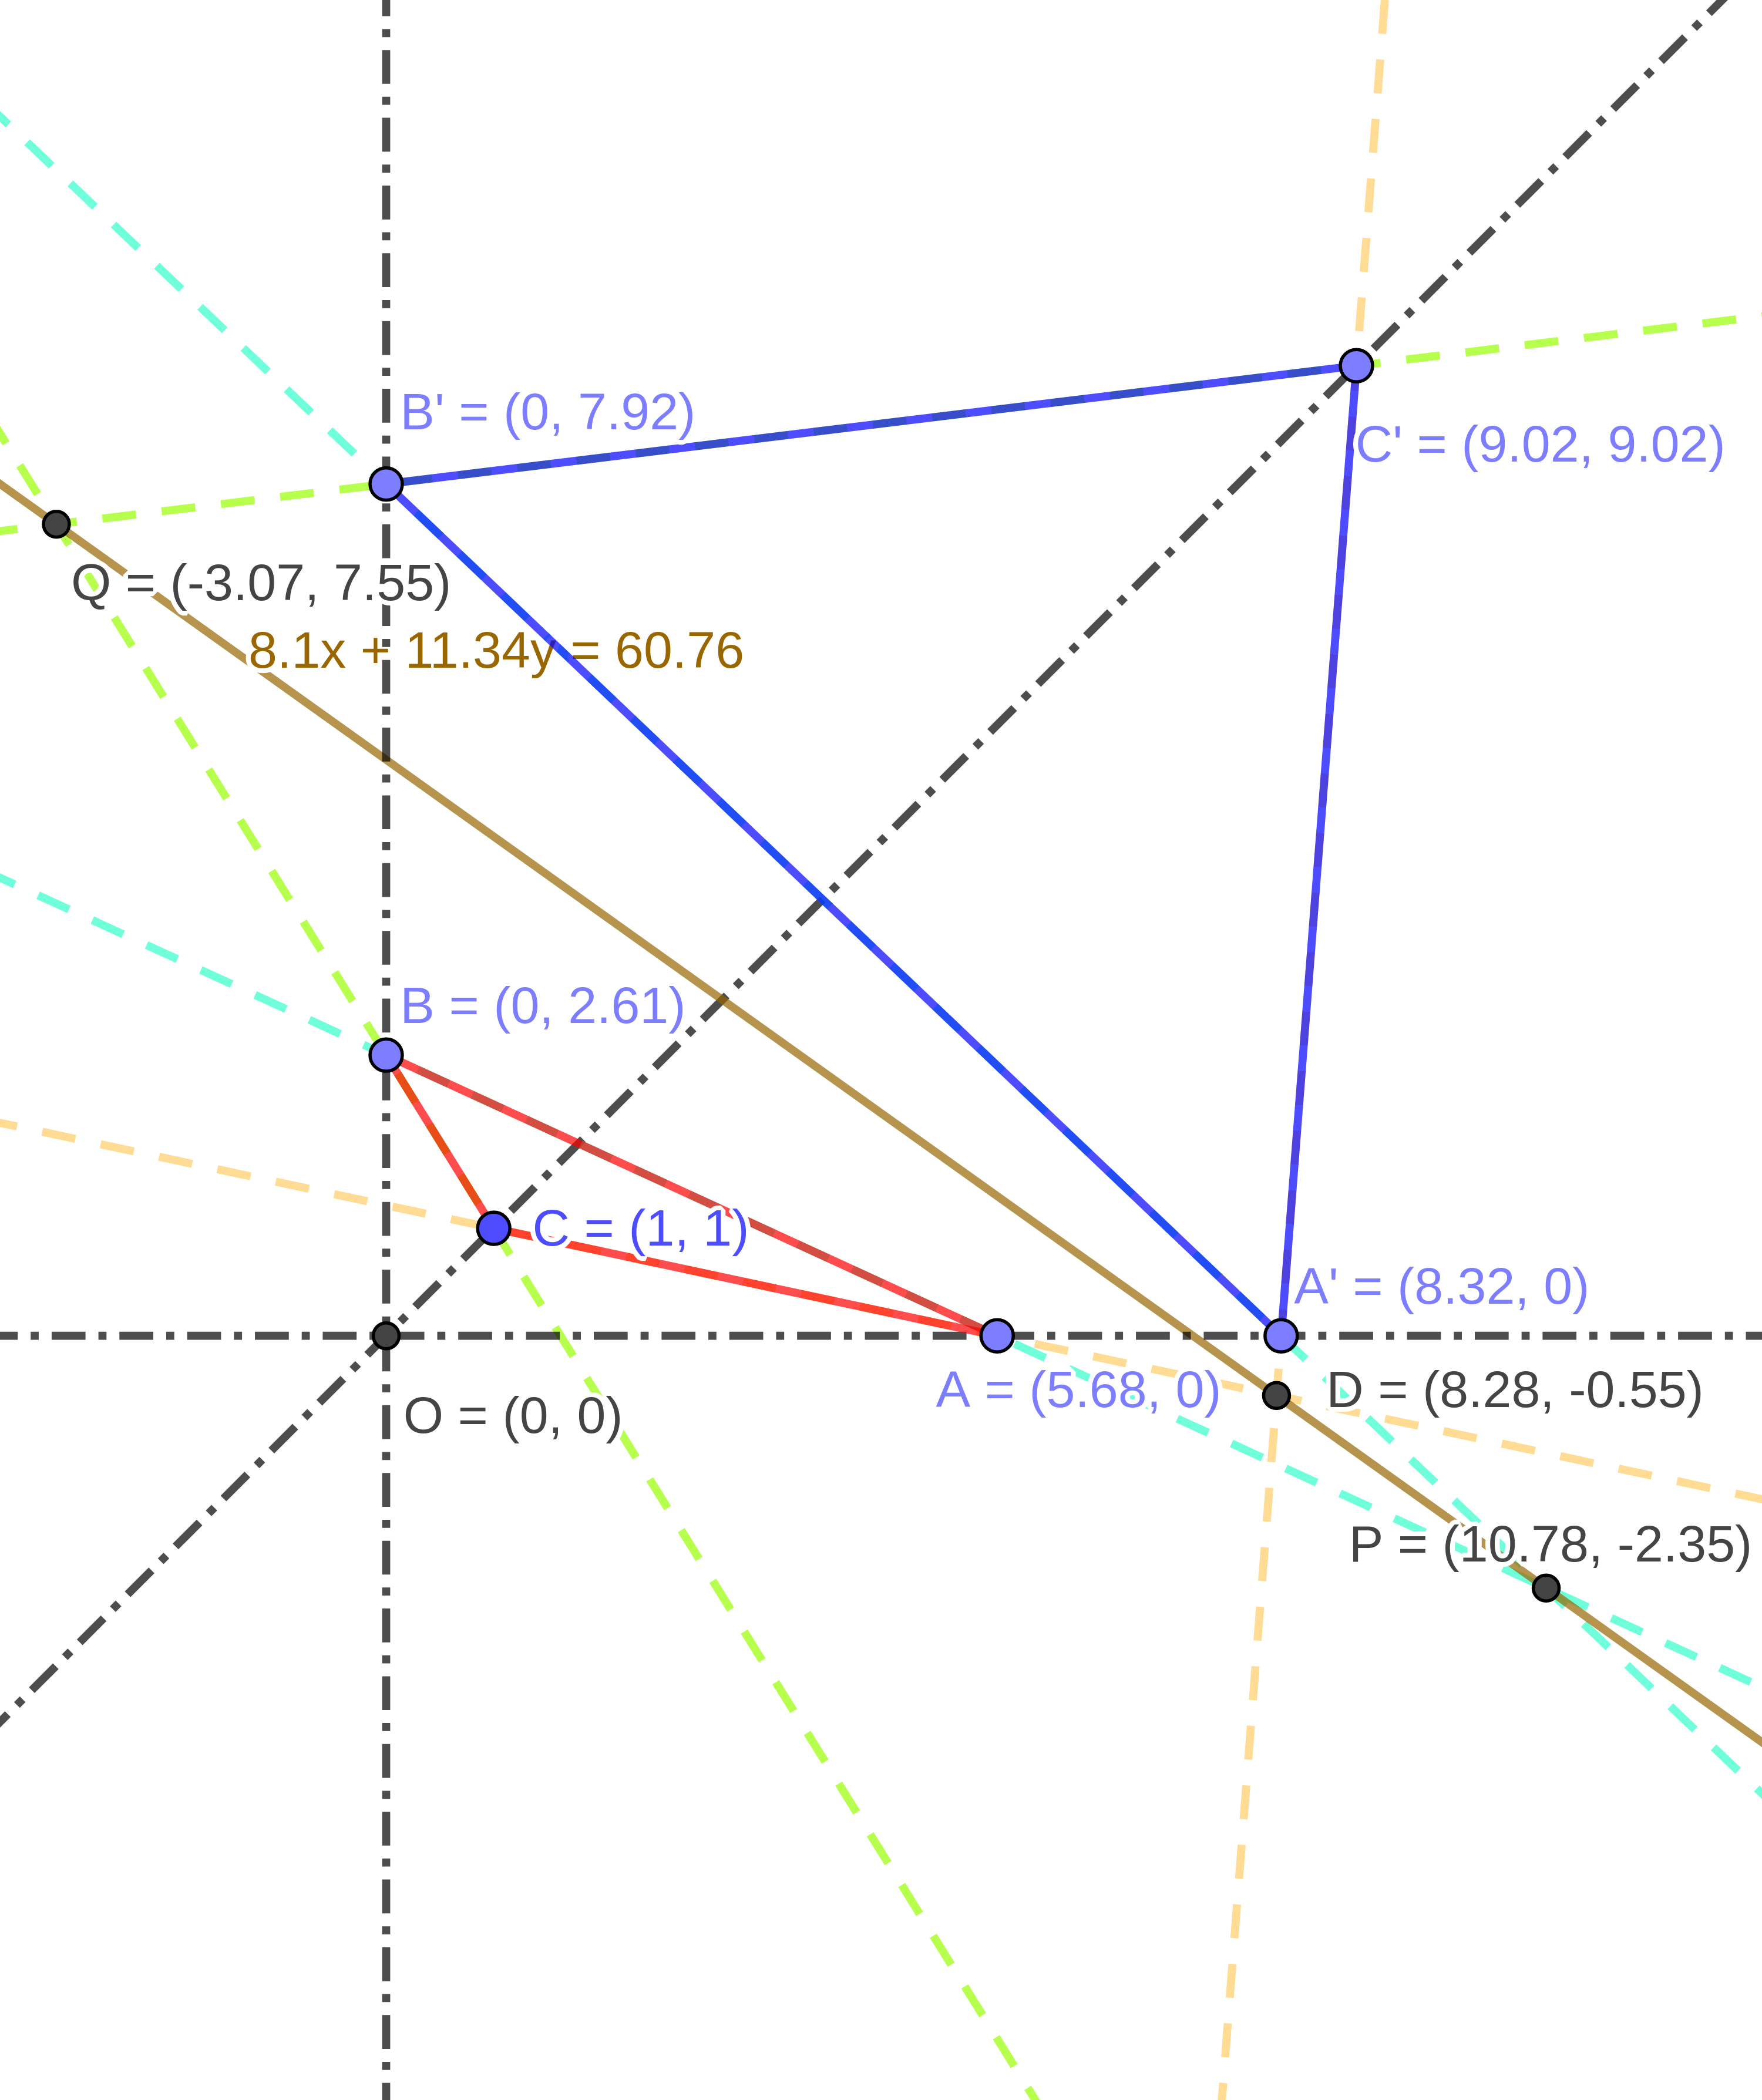
\includegraphics{Problema_02.png}
  \\
  Ejemplo del resultado obtenido.
  Imagen extra\'{\i}da del archivo Problema\_02(Desargues)(01).ggb
 \end{center}

\end{solucion}

 \item \begin{enunciado}
 Sean $A$ y $B$ dos matrices reales, ambas cuadradas y de igual tama\~no. Compru\'ebese que:
 \begin{enumerate}[$a$)]
  \item Si una, al menos, de las matrices $A$ o $B$ es regular, entonces $AB$ y $BA$ tienen el mismo polinomio caracter\'{\i}stico.
  \item Si $A$ y $B$, ambas, singulares, entonces $AB$ y $BA$ tienen, tambi\'en, el mismo polinomio caracter\'{\i}stico (indicaci\'on: recurrir al resultado anterior aplicando a $A$ y $B' = B + \varepsilon I$ y h\'allase luego que $\varepsilon$ tiende a cero).
 \end{enumerate}

\end{enunciado}

\begin{solucion}
 Sea $C$ una matriz regular, entonces existe $C^{-1}$, $\det C \neq 0$ y $\det (C^{-1}) = \left( \det C \right)^{-1}$, entonces:
 \begin{enumerate}[a)]
  \item Si $C$ es matriz regular, entonces
  \begin{eqnarray*}
   \det (AB - \lambda I) & = & 1\cdot \det (AB - \lambda I) = \det C \det (C^{-1}) \det (AB - \lambda I) = \\
   & = &\det (C^{-1}) \det (AB - \lambda I) \det C = \det \left[ C^{-1}(AB - \lambda I) C \right] \\
   & = & \det (C^{-1}ABC - \lambda C^{-1}I C) \\
   & = & \det (C^{-1}ABC - \lambda I) \\ 
  \end{eqnarray*}
  Entonces, si $A$ es regular, se toma $C = A$ y $\det(AB-\lambda I) = \det(A^{-1}ABA - \lambda I) = \det(IBA - \lambda I) = \det (BA - \lambda I)$; por otro lado, si $B$ es regular, se toma $C = B^{-1}$, entonces $C^{-1} = B$ y $\det(AB-\lambda I) = \det (BABB^{-1} - \lambda I) = \det (BAI - \lambda I) = \det(BA - \lambda I)$. \\
  Por lo tanto, en cualquier caso si $A$ o $B$ es regular, entonces el polinomio caracter\'{\i}stico de $AB$, que se obtiene como $\det(AB - \lambda I) = 0$ es equivalente a $\det(BA - \lambda I) = 0$ que es el polinomio caracter\'{\i}stico de $BA$, es decir: los polinomios caracter\'{\i}sticos de AB y BA son iguales.
  
  \item Sean $C$ y $D$ matrices cuadradas de tama\~no $2n\times 2n$, suponiendo que el tama\~no de las matrices A y B es de $n\times n$, que se pueden expresar por bloques como:
  \begin{equation*}
   C = 
   \begin{pmatrix}
    \lambda I & A \\
    B         & I
   \end{pmatrix}
   \qquad \text{y} \qquad 
   D = 
   \begin{pmatrix}
    -I & 0 \\ 
     B & -\lambda I
   \end{pmatrix}
  \end{equation*}
  entonces
  \begin{equation*}
   CD = 
   \begin{pmatrix}
    AB-\lambda I & \lambda -A \\
    0            & -\lambda I
   \end{pmatrix}
   \qquad \text{y} \qquad 
   DC = 
   \begin{pmatrix}
    -\lambda I & -A \\
    0          & BA - \lambda I
   \end{pmatrix}
  \end{equation*}
  Por lo tanto, usando el c\'alculo de determinantes por bloques, se tiene que:
  \begin{equation*}
   \det (CD) = \det
   \begin{pmatrix}
    AB-\lambda I & \lambda -A \\
    0                    & -\lambda I
   \end{pmatrix}
   = \det(AB-\lambda I)\det(-\lambda I) = (-\lambda)^n \det (AB - \lambda)
  \end{equation*}
  y 
  \begin{equation*}
   \det(DC) = \det
   \begin{pmatrix}
    -\lambda I & -A \\
    0          & BA - \lambda I
   \end{pmatrix}
   = \det(- \lambda I) \det(BA - \lambda I) = (-\lambda)^n \det(BA - \lambda I)
  \end{equation*}
  y como $\det (CD) = \det (DC)$, se concluye que $\det(AB - \lambda I) = \det (BA - \lambda I)$, que es lo que se quer\'{\i}a comprobar.${}_{\blacksquare}$




 \end{enumerate}
\end{solucion}


 \item \begin{enunciado}
 Sean $A_1A_2A_3$ un tri\'angulo del plano af\'{\i}n $E_2$ y sean $B_1$, $B_2$ y $B_3$ puntos situados en los segmentos $A_2A_3$, $A_3A_1$ y $A_1A_2$, respectivamente. Pru\'ebese que las tres rectas $A_1B_1$, $A_2B_2$ y $A_3B_3$ pasan, las tres, por un mismo punto si y s\'olo si el producto de las razones simples (v\'ease el problema precedente) $\left( B_1A_2A_3 \right)$, $\left( B_2A_3A_1 \right)$ y $\left( B_3A_1A_2 \right)$ vale $-1$ (teorema de Ceva).
\end{enunciado}

\begin{solucion}
 
\end{solucion}


 \item \begin{enunciado}
 Hallar los autovalores y los subespacios propios del endomorfismo $f:\mathbb{R}^3 \rightarrow \mathbb{R}^3$ que, en la base can\'onica, tiene asociada la matriz $A$:
 \begin{equation*}
  A = 
  \begin{bmatrix}
   1 &  1 & 0 \\
   3 & -1 & 6 \\
   1 & -1 & 3
  \end{bmatrix}
 \end{equation*}
 Anal\'{\i}cese si $f$ es diagonalizable.
\end{enunciado}

\begin{solucion}
 Calculando $\det (A - \lambda I)$, se tiene que:
 \begin{eqnarray*}
  \det (A - \lambda I) & = & 
  \begin{vmatrix}
   1-\lambda &  1         & 0 \\
   3         & -1-\lambda & 6 \\
   1         & -1         & 3-\lambda
  \end{vmatrix} \\ 
  & = & (1-\lambda)
  \begin{vmatrix}
   -1-\lambda & 6         \\
   -1         & 3-\lambda
  \end{vmatrix}
  - 3
  \begin{vmatrix}
    1 & 0         \\
   -1 & 3-\lambda
  \end{vmatrix}
  + 
  \begin{vmatrix}
    1         & 0 \\
   -1-\lambda & 6
  \end{vmatrix} \\ 
  & = & (1-\lambda)\left[ (-1-\lambda)(3-\lambda) + 6 \right] - 3(3-\lambda) + (6) \\ 
  & = & (1-\lambda)(-3-2\lambda + \lambda^2 + 6) - 9 + 3\lambda + 6 = (1-\lambda)(\lambda^2 - 2\lambda + 3) + 3\lambda - 3 \\
  & = & (-\lambda^3 + 3\lambda^2 -5\lambda + 3) + 3\lambda - 3 = -\lambda^3 +3\lambda^2 -2\lambda \\
  & = & -\lambda(\lambda^2 - 3\lambda + 2) = -\lambda(\lambda - 2)(\lambda - 1) 
 \end{eqnarray*}
 Por lo tanto, $\det(A-\lambda I) = 0$ si y s\'olo si $\lambda \in \{ 0, 1, 2 \}$. Luego, como los autovalores de $A$ son los mismo que los de $f$, sin importar la base, se tiene que $\lambda_0 = 0$, $\lambda_1 = 1$ y $\lambda_2 = 2$ son los autovalores de $f$.
 \par 
 Para hallar los subespacios propios de $f$, basta con encontrar los vectores $\overline{x}$ que cuyo vector de coordenadas en la base can\'onica, $X = (x, y, z)^t$, cumplan que $AX = \lambda_iX$ para cada $i \in \{ 0, 1, 2\}$.
 \par 
 Para el caso $\lambda = 0$, se tiene que
 \begin{equation*}
  AX = O \Leftrightarrow 
  \left.
  \begin{matrix}
    x & +y &     & = 0 \\
   3x & -y & +6z & = 0 \\
  \end{matrix}
  \right\} \Leftrightarrow
  \left.
  \begin{matrix}
   x  & = -y \\
   4x & +6z = 0
  \end{matrix}
  \right\} \Leftrightarrow
  \left.
  \begin{matrix}
   x  & = -y \\
   x & = -\frac{3}{2}z
  \end{matrix}
  \right\} \Leftrightarrow
  \left.
  \begin{matrix}
   x & = -3\alpha \\
   y & =  3\alpha \\
   z & =  2\alpha
  \end{matrix}
  \right\}
 \end{equation*}
 Por lo tanto $V_{\lambda_0} = \{ (-3\alpha, 3\alpha, 2\alpha) \in \mathbb{R}^3| \alpha \in \mathbb{R} \}$. \par 
 Para el caso $\lambda = 1$, se tiene que:
 \begin{equation*}
  AX = X \Leftrightarrow 
  \left.
  \begin{matrix}
    x & +y &     & = x \\
   3x & -y & +6z & = y \\
  \end{matrix}
  \right\} \Leftrightarrow
  \left.
  \begin{matrix}
   y  & = 0 \\
   3x & +6z = 0
  \end{matrix}
  \right\} \Leftrightarrow
  \left.
  \begin{matrix}
   y & = 0 \\
   x & = -2z
  \end{matrix}
  \right\} \Leftrightarrow
  \left.
  \begin{matrix}
   x & = -2\alpha \\
   y & = 0 \\
   z & = \alpha
  \end{matrix}
  \right\}
 \end{equation*}
 Por lo tanto $V_{\lambda_1} = \{ (-2\alpha, 0, \alpha) \in \mathbb{R}^3 | \alpha \in \mathbb{R} \}$.
 \par 
 Y, para el caso $\lambda = 2$, se tiene que: 
 \begin{equation*}
  AX = 2X \Leftrightarrow 
  \left.
  \begin{matrix}
    x & +y &     & = 2x \\
   3x & -y & +6z & = 2y \\
  \end{matrix}
  \right\} \Leftrightarrow
  \left.
  \begin{matrix}
   y  & = x \\
   2x & +6z = 2x
  \end{matrix}
  \right\} \Leftrightarrow
  \left.
  \begin{matrix}
   x & = y \\
   z & = 0
  \end{matrix}
  \right\} \Leftrightarrow
  \left.
  \begin{matrix}
   x & = \alpha \\
   y & = \alpha \\
   z & = 0
  \end{matrix}
  \right\}
 \end{equation*}
 Por lo tanto, $V_{\lambda_2} = \{(\alpha, \alpha, 0) \in \mathbb{R} | \alpha \in \mathbb{R} \}$.
 \par 
 Finalmente, como se tiene que la dimensi\'on del espacio es $3$ y $f$ tiene $3$ autovalores reales distintos, se concluye que $f$ es diagonalizable; a saber, la matriz diagonal $D = P^{-1}AP$ de $f$ se obtiene respecto a la nueva base $\left( (-3, 3, 2), (2, 0, -1), (1, 1, 0) \right)$ donde $D$ y $P$ son:
 \begin{equation*}
  D = 
  \begin{pmatrix}
   0 & 0 & 0 \\
   0 & 1 & 0 \\
   0 & 0 & 2
  \end{pmatrix}
  \qquad \text{y} \qquad 
  P = 
  \begin{pmatrix}
   -3 &  2 & 1 \\
    3 &  0 & 1 \\
    2 & -1 & 0
  \end{pmatrix}
 \end{equation*}
 que es a lo que se quer\'{\i}a llegar.${}_{\blacksquare}$ 
\end{solucion}


 \item \begin{enunciado}
 Hallar los autovalores y los subespacios propios del endomorfismo $f:\mathbb{R}^3 \rightarrow \mathbb{R}^3$ que, respecto de la base can\'onica, tiene asociada la siguiente matriz $A$:
 \begin{equation*}
  A = 
  \begin{bmatrix}
    1 & 1 & -1 \\
    1 & 1 &  1 \\
   -1 & 1 &  1
  \end{bmatrix}
 \end{equation*}
 Anal\'{\i}cese si $f$ es diagonalizable.
\end{enunciado}

\begin{solucion}
 Se proceder\'a a calcular el polinomio caracter\'{\i}stico de $f$ a trav\'es de $A$:
 \begin{eqnarray*}
  \det(A - \lambda I) & = & 
  \begin{vmatrix}
   1-\lambda & 1         & -1        \\
   1         & 1-\lambda &  1        \\
   -1        & 1         & 1-\lambda
  \end{vmatrix} \\
  & = & (1-\lambda)
  \begin{vmatrix}
   1 - \lambda & 1           \\
   1           & 1 - \lambda
  \end{vmatrix}
  -
  \begin{vmatrix}
   1 & -1          \\
   1 & 1 - \lambda
  \end{vmatrix}
  -
  \begin{vmatrix}
   1           & -1 \\
   1 - \lambda &  1
  \end{vmatrix} \\ 
  & = & (1-\lambda)\left[ (1-\lambda)^2 - 1 \right] - \left[ (1-\lambda) + 1 \right] - \left[ 1 + (1-\lambda) \right] \\
  & = & (1-\lambda)(\lambda^2 - 2\lambda) + (\lambda - 2) + (\lambda-2) \\ 
  & = & (-\lambda^3 + 3\lambda^2 -2\lambda) + 2\lambda - 4 \\ 
  & = & -\lambda^3 + 3\lambda^2 - 4 
  = -(\lambda^3 - 3\lambda^2 + 4) \\
  & = & -(\lambda+1)(\lambda^2 - 4\lambda +  4) \\ 
  & = & -(\lambda + 1)(\lambda - 2)^2
 \end{eqnarray*}
 Por lo tanto, $\det (A - \lambda I) = 0$ para los autovalores de $f$: $\lambda_1 = -1$, con multiplicidad algebraica $m_1 = 1$, y $\lambda_2 = 2$, con multiplicidad algebraica $m_2 = 2$.
 \par 
 Para hallar los subespacios propios de $f$, basta con encontrar los vectores $\overline{x}$ cuyo vector de coordenadas en la base can\'onica $X = (x, y, z)^t$, cumpla que $AX = \lambda_i X$ para cada $i \in \{ 1, 2\}$.
 \par 
 Para el caso $\lambda_1 = -1$, se tiene que $(A + I)X = 0$ es equivalente a:
 \begin{equation*}
  \left. 
  \begin{matrix}
   2x & +  y & - z & = 0 \\
    x & + 2y & + z & = 0
  \end{matrix}
  \right\}
  \Leftrightarrow 
  \left. 
  \begin{matrix}
   2x & +  y & - z & = 0 \\
    x & + 2y & + z & = 0 \\
   x & + y & = 0 \\
  \end{matrix}
  \right\}
  \Leftrightarrow 
  \left. 
  \begin{matrix}
   x & - z & = 0 \\
   y & + z & = 0 \\
  \end{matrix}
  \right\}
  \Leftrightarrow 
  \left. 
  \begin{matrix}
   x = \alpha \\
   y = - \alpha \\
   z = \alpha
  \end{matrix}
  \right\}
 \end{equation*}
 Por lo tanto $V_{\lambda_1} = \left\{ (\alpha, -\alpha, \alpha) \in \mathbb{R}^3 | \, \alpha \in \mathbb{R} \right\}$.
 \par 
 Para el caso $\lambda_2 = 2$, se tiene que $(A - 2I)X = 0$ es equivalente al sistema de tres ecuaciones: $-x + y -z = 0$, $x-y+z = 0$ y $-x+y-z = 0$, los cuales son todos equivalentes entre s\'{\i}. Por lo tanto, $V_{\lambda_2} = \left\{ (x,y,z) \in \mathbb{R}^3 | x-y+z = 0 \right\} = \left\{ (\alpha - \beta, \alpha, \beta ) \in \mathbb{R}^3 | \, \alpha, \beta \in \mathbb{R} \right\}$.
 \par 
 Finalmente, como se tiene que las multiplicidades algebraica suman $m_1 + m_2 = 1 + 2 = 3 = \dim \mathbb{R}^3$ y las multiplicidades geom\'etricas cumplen que $d_1 = 1 = m_1$ y $d_2 = 2 = m_2$, entonces se concluye que $f$ s\'{\i} es diagonalizable; a saber, la matriz diagonal $D = P^{-1}AP$ de $f$ se obtiene respecto de la nueva base $\left( (1, -1, 1), (1, 1, 0), (-1, 0, 1) \right)$ donde $D$ y $P$ son:
 \begin{equation*}
  D = 
  \begin{pmatrix}
   -1 & 0 & 0 \\
    0 & 2 & 0 \\
    0 & 0 & 2 
  \end{pmatrix}
  \qquad \text{y} \qquad 
  P = 
  \begin{pmatrix}
    1 & 1 & -1 \\
   -1 & 1 &  0 \\
    1 & 0 &  1
  \end{pmatrix}
 \end{equation*}
 que es a lo que se quer\'{\i}a llegar.${}_{\blacksquare}$
\end{solucion}


 \item \begin{enunciado}
 Hallar los autovalores y los subespacios propios del endomorfismo $f:V \rightarrow V$ (donde $V$ es un espacio vectorial real de dimensi\'on $4$) que, en cierta base dada $(\overline{e}_1, \overline{e}_2, \overline{e}_3, \overline{e}_4)$ de $V$, tiene asociada la siguiente matriz $A$:
 \begin{equation*}
  A = 
  \begin{bmatrix}
    3 &  3 & 0 &  1 \\
   -1 & -1 & 0 & -1 \\
    1 &  2 & 1 &  1 \\
    2 &  4 & 0 &  3
  \end{bmatrix}
 \end{equation*}
 Anal\'{\i}cese si $f$ es diagonalizable.
\end{enunciado}

\begin{solucion}
 Se proceder\'a a calcular el polinomio caracter\'{\i}stico de $f$ a trav\'es de la matriz asociada a $f$ en la base $\beta = (\overline{e}_1, \overline{e}_2, \overline{e}_3, \overline{e}_4)$, $A$, como sigue:
 \begin{eqnarray*}
  \det(A-\lambda I) & = &
  \begin{vmatrix}
    3 - \lambda &  3           & 0     &          1           \\
   -1           & -1 - \lambda & 0     &          -1           \\
    1           &  2           & 1 - \lambda &  1           \\
    2           &  4           & 0     &          3 - \lambda 
  \end{vmatrix} \\
  & = & (1-\lambda)
  \begin{vmatrix}
    3 - \lambda &  3           &  1 \\
   -1           & -1 - \lambda & -1 \\
    2           &  4           &  3 - \lambda
  \end{vmatrix} \\ 
  & = & (1-\lambda)\left[ (3-\lambda)
  \begin{vmatrix}
   -1 - \lambda & -1           \\
    4           &  3 - \lambda
  \end{vmatrix}
  +
  \begin{vmatrix}
   3 & 1           \\
   4 & 3 - \lambda
  \end{vmatrix}
  + 2
  \begin{vmatrix}
    3           &  1 \\
   -1 - \lambda & -1
  \end{vmatrix}
  \right] \\
  & = & (1-\lambda)\left[ (3-\lambda)(\lambda^2 - 2 \lambda - 3 + 4) + (-3\lambda + 9 - 4) + 2(-3 + 1+\lambda) \right] \\ 
  & = & (1-\lambda)\left[ (3-\lambda)(\lambda^2 - 2\lambda +1 ) + (-3\lambda + 5) + 2(\lambda - 2) \right] \\
  & = & (1 - \lambda)\left[ (-\lambda^3 + 5\lambda^2 - 7\lambda + 3) + (-3\lambda + 5) + (2\lambda - 4) \right] \\
  & = & (1 - \lambda)(-\lambda^3 + 5\lambda^2 - 8\lambda + 4) \\
  & = & (\lambda - 1)(\lambda^3 - 5\lambda^2 + 8\lambda - 4) \\
  & = & (\lambda - 1)^2(\lambda^2 - 4\lambda + 4) \\ 
  & = & (\lambda - 1)^2(\lambda - 2)^2
 \end{eqnarray*}
 Por lo tanto, $\det (A - \lambda I) = 0$ para los autovalores, de $A$ que tambi\'en son de $f$: $\lambda_1 = 1$, con multiplicidad algebraica $m_1 = 2$, y $\lambda_2 = 2$, con multiplicidad algebraica $m_2 = 2$.
 \par 
 Para hallar los subespacios propios de $f$ se usar\'a nuevamente la matriz asociada a $f$ en la base $\beta$, calculando los vectores coordenadas $X = (x_1, x_2, x_3, x_4)^t$ de un vector gen\'erico $\overline{x}$ en la base $\beta$ que cumplan que $AX = \lambda_iX$ para cada $i \in \{ 1, 2 \}$. 
 \par 
 Para el caso $\lambda_1 = 1$, se tiene que $(A - I)X = 0$ es equivalente al sistema de ecuaciones:
 \begin{equation*}
  \begin{matrix}
   2x_1 & +3x_2 & + x_4 & = 0 \\
   -x_1 & -2x_2 & - x_4 & = 0 \\
    x_1 & +2x_2 & + x_4 & = 0 \\
   2x_1 & +4x_2 & +2x_4 & = 0
  \end{matrix}
 \end{equation*}
 en el cual la segunda, tercera y cuarta ecuaci\'on son equivalentes, por lo que se reduce a un sistema de dos ecuaciones el cual se resuelve como sigue:
 \begin{equation*}
  \left.
  \begin{matrix}
   2x_1 & +3x_2 & + x_4 & = 0 \\
   -x_1 & -2x_2 & - x_4 & = 0
  \end{matrix}
  \right\}
  \Leftrightarrow 
  \left. 
  \begin{matrix}
   2x_1 & +3x_2 & + x_4 & = 0 \\
   -x_1 & -2x_2 & - x_4 & = 0 \\
   x_1  & + x_2 &       & = 0
  \end{matrix}
  \right\}
  \Leftrightarrow 
  \left. 
  \begin{matrix}
   x_1 &       & = - x_2 \\
   x_2 & + x_4 & = 0 
  \end{matrix}
  \right\}
  \Leftrightarrow
  \left. 
  \begin{matrix}
   x_1 = \alpha \\
   x_2 = -\alpha \\
   x_3 = \beta \\
   x_4 = \alpha
  \end{matrix}
  \right\}
 \end{equation*}
 Por lo tanto, $V_{\lambda_1} = \left\{ \overline{x} \in V |\, \overline{x} = \alpha\overline{e}_1 - \alpha\overline{e}_2 + \beta\overline{e}_3 + \alpha\overline{e}_4, \text{ con } \alpha, \beta \in \mathbb{R} \right\}$.
 \par
 Para el caso $\lambda_2 = 2$, se tiene que $(A-2I)X = 0$ es equivalente al sistema de ecuaciones:
 \begin{equation*}
  \begin{matrix}
    x_1 & +3x_2 &      & +x_4 & = 0 \\
   -x_1 & -3x_2 &      & -x_4 & = 0 \\
    x_1 & +2x_2 & -x_3 & +x_4 & = 0 \\
   2x_1 & +4x_2 &      & +x_4 & = 0
  \end{matrix}
 \end{equation*}
 en el cual la segunda y tercera ecuaci\'on son equivalentes, por lo que se reduce al sistema de tres ecuaciones el cual se resuelve como sigue:
 \begin{equation*}
  \left.
  \begin{matrix}
    x_1 & +3x_2 &      & +x_4 & = 0 \\
    x_1 & +2x_2 & -x_3 & +x_4 & = 0 \\
   2x_1 & +4x_2 &      & +x_4 & = 0
  \end{matrix}
  \right\}
  \Leftrightarrow 
  \left. 
  \begin{matrix}
    x_1 & +3x_2 &      & +x_4 & = 0 \\
    x_1 & +2x_2 & -x_3 & +x_4 & = 0 \\
   2x_1 & +4x_2 &      & +x_4 & = 0 \\
    x_1 & + x_2 &      &      & = 0
  \end{matrix}
  \right\}
  \Leftrightarrow 
  \left. 
  \begin{matrix}
    x_1 &      &      & = -x_2 \\
   2x_2 &      & +x_4 & = 0 \\
    x_2 & -x_3 & +x_4 & = 0
  \end{matrix}
  \right\}
 \end{equation*}
 \begin{equation*}
  \Leftrightarrow 
  \left. 
  \begin{matrix}
    x_1 &      & = - x_2 \\
    x_4 &      & = -2x_2 \\
   -x_2 & -x_3 & = 0     
  \end{matrix}
  \right\}
  \Leftrightarrow 
  \left. 
  \begin{matrix}
   x_1 & = & - \alpha \\ 
   x_2 & = &   \alpha \\
   x_3 & = & - \alpha \\
   x_4 & = & -2\alpha 
  \end{matrix}
  \right\}
 \end{equation*}
 Por lo tanto, $V_{\lambda_2} = \left\{ \overline{x} \in V | \, \overline{x} = -\alpha\overline{e}_1 + \alpha\overline{e}_2 - \alpha\overline{e}_3 - 2\alpha\overline{e}_4, \text{ con } \alpha\in\mathbb{R} \right\}$.
 \par 
 Finalmente, aunque las multiplicidades algebraicas sumen la dimensi\'on del espacio, es decir $m_1 + m_2 = 2 + 2 = 4 = \dim V$, no ocurre que las dimensiones geom\'etricas sean iguales a sus correspondientes multiplicidades algebraicas, esto es $d_1 = 2 = m_1$, pero $d_2 = 1 \neq 2 = m_1$. 
 Por lo tanto, por teorema, se sigue que $f$ no es diagonalizable, que es a lo que se quer\'{\i}a llegar.${}_{\blacksquare}$
\end{solucion}


 \item \begin{enunciado}
 Hallar los autovalores y los subespacios propios de la matriz $A$, de tama\~no $n\times n$ con $n \geq 2$:
 \begin{equation*}
  A = 
  \begin{matrix}
%    \begin{matrix}
%     \phantom{1+a} & \phantom{1+a} & \phantom{1+a} & \cdots & \phantom{1+a}
%    \end{matrix}
   \begin{bmatrix}
    \begin{matrix}
     1 + a & 1     & 1     & \cdots & \phantom{+} 1\phantom{a} \\
     1     & 1 + a & 1     & \cdots & \phantom{+} 1\phantom{a} \\
     1     & 1     & 1 + a & \cdots & \phantom{+} 1\phantom{a}
    \end{matrix} \\
    \dotfill\hspace{-2pt}\dotfill\hspace{-2pt}\dotfill\hspace{-2pt}\dotfill\hspace{-2pt}\dotfill \\
    \dotfill\hspace{-2pt}\dotfill\hspace{-2pt}\dotfill\hspace{-2pt}\dotfill\hspace{-2pt}\dotfill \\
    \begin{matrix}
     \phantom{+1} 1\phantom{1a} & \phantom{+} 1\;\phantom{a} & \phantom{+} 1\;\phantom{a} & \cdots & 1 + a 
    \end{matrix}
   \end{bmatrix}
  \end{matrix}
 \end{equation*}
 Anal\'{\i}cese si $A$ es diagonalizable por semejanza.
\end{enunciado}

\begin{solucion}
 Para hallar los autovalores de A, primero se proceder\'a a calcular el polinomio caracter\'{\i}stico, esto es, se proceder\'a a calcular $\det (A - \lambda I)$, el cual se puede escribir como:
 \begin{equation*}
  \begin{vmatrix}
   1+a-\lambda & 1               &    1           & \cdots & 1 \\ 
   1           & 1 + a - \lambda &    1           & \cdots & 1 \\
   1           & 1               & 1 + a - \lambda & \cdots & 1 \\
   \vdots & \vdots & \vdots & \ddots & \vdots \\
   1           & 1               &    1           & \cdots & 1 + a - \lambda 
  \end{vmatrix}
 \end{equation*}
 Usando la propiedad del determinante que dice que si a un rengl\'on, o una columna, se le suma una combinaci\'on lineal de los dem\'as renglones, o columnas, respectivamente, entonces el valor del determinante no cambia. Entonces, al sumar al primer rengl\'on cada uno de los otros $n-1$ renglones, el valor del determinante no cambia y el nuevo determinante se puede escribir como:
 \begin{equation*}
  \begin{vmatrix}
   n + a - \lambda & n + a - \lambda & n + a - \lambda & \cdots & n + a - \lambda \\ 
   1               & 1 + a - \lambda & 1               & \cdots & 1 \\
   1               & 1               & 1 + a - \lambda & \cdots & 1 \\
   \vdots & \vdots & \vdots & \ddots & \vdots \\
   1               & 1               & 1               & \cdots & 1 + a - \lambda
  \end{vmatrix}
 \end{equation*}
 Luego, como el primer rengl\'on es m\'ultiplo de $n + a - \lambda$, usando la propiedad de determinantes que dice que si un rengl\'on o columna es m\'ultiplo de cierto factor, entonces el determinantes es igual al producto de \'este por el determinante de la matriz que se obtiene al dividir en el rengl\'on o columna correspondiente el factor donde todos los valores eran m\'ultiplos. Entonces el determinante es igual a:
 \begin{equation*}
  (n+a-\lambda)\cdot 
  \begin{vmatrix}
   1 & 1               & 1            &         \cdots & 1 \\ 
   1 & 1 + a - \lambda & 1               &         \cdots & 1 \\
   1 & 1               & 1 + a - \lambda & \cdots & 1 \\
   \vdots & \vdots & \vdots & \ddots & \vdots \\
   1 & 1               & 1               & \cdots & 1 + a - \lambda
  \end{vmatrix}
 \end{equation*}
 Entonces, volviendo a aplicar la propiedad en donde el determinante queda invariante ante la suma de un rengl\'on o columna con una combinaci\'on lineal del resto de renglones o columnas, respectivamente, entonces al restar a cada rengl\'on $i$, con $2 \leq i \leq n$, el primer rengl\'on, se obtiene que el valor del determinante buscado es igual a
 \begin{equation*}
  (n+a-\lambda)\cdot 
  \begin{vmatrix}
   1 & 1           & 1           &         \cdots & 1 \\ 
   0 & a - \lambda & 0           &         \cdots & 0 \\
   0 & 0           & a - \lambda & \cdots & 0 \\
   \vdots & \vdots & \vdots & \ddots & \vdots \\
   0 & 0           & 0           & \cdots & a - \lambda
  \end{vmatrix}
 \end{equation*}
 Finalmente, usando la propiedad de determinantes que dice que en una matriz triangular, el determinante de dicha matriz es el producto de sus elementos en la diagonal, se obtiene que el valor buscado es $\det(A - \lambda I) = (n + a - \lambda)(a - \lambda)^n$. Por lo tanto, la ecuaci\'on caracter\'{\i}stica $\det(A - \lambda I) = 0$ se resuelve para los autovalores de $A$: $\lambda_1 = n+a$, con multiplicidad algebraica $m_1 = 1$, y $\lambda_2 = a$ con multiplicidad algebraica $m_2 = n - 1$.
 \par 
 Para hallar los subespacios propios, se procede a buscar los valores $X = (x_1, x_2, \ldots, x_n)^t$ tales que $AX = \lambda_i X$, o lo que es equivalente, $(A-\lambda_i I)X = O$, para cada $i \in \{ 1, 2 \}$.
 \par 
 Para el caso $\lambda_1 = n+a$, se tiene que en la ecuaci\'on caracter\'{\i}stica, $[A - (n+a)I]X = O$, la $i-$\'esima ecuaci\'on corresponde a
 \begin{equation*}
  (1-n)x_i + \sum_{\substack{k=1\\k\neq i}}^n x_k = 0, \qquad \text{para } i \in \mathbb{N}\cap[1, n]
 \end{equation*}
 o lo que es equivalente:
 \begin{equation*}
  \sum_{k=1}^n x_k - nx_i = 0
  \Leftrightarrow 
  \sum_{k=1}^n x_k = nx_i
  , \qquad \text{para } i \in \mathbb{N}\cap [1,n]
 \end{equation*}
 Luego entonces, cada $nx_i$ es igual a la suma de todas las coordenadas, para $1\leq i \leq n$, entonces $nx_1 = nx_2 = \cdots = nx_n$, o lo que es lo mismo $x_1 = x_2 = \cdots = x_n$. Por lo tanto $V_{\lambda_1} = \left\{ (\alpha, \alpha, \cdots, \alpha) \in \mathbb{R}^n | \, \alpha \in \mathbb{R} \right\} = \left< (1, 1, \cdots , 1) \right>$.
 \par 
 Para el caso $\lambda_2 = a$, se tiene que en la ecuaci\'on caracter\'{\i}stica $(A - aI)X = O$, cada ecuaci\'on es id\'entica e igual a
 \begin{equation*}
  \sum_{i=1}^n x_i = 0
 \end{equation*}
 Por lo tanto, $V_{\lambda_2} = \left\{ (x_1, x_2, \cdots, x_n) \in \mathbb{R}^n | \, x_1 + x_2 + \cdots + x_n = 0 \right\}$.
 \par 
 Finalmente, como las multiplicidades algebraicas de las ra\'{\i}ces del polinomio caracter\'{\i}stico suman la dimensi\'on del espacio, esto es $m_1 + m_2 = 1 + (n-1) = n = \dim \mathbb{R}^n$, y, adem\'as, las multiplicidades geom\'etricas coinciden con las multiplicidades algebraicas, esto es $d_1 = 1 = m_1$ y $d_2 = n-1 = m_2$, entonces, por teorema, se concluye que $A$ s\'{\i} es diagonalizable por semejanza; a saber, la matriz diagonal $D = P^{-1}AP$ se obtiene respecto de la nueva base $\beta' = \left\{ (1, 1, \cdots, 1), (1, -1, 0, \cdots, 0), (1, 0, -1, 0, \cdots, 0), \ldots, (1, 0, 0, \cdots, 0, -1) \right\}$ donde $D$ y $P$ son:
 \begin{equation*}
  D = 
  \begin{bmatrix}
   n+a & 0 & 0 & \cdots & 0 \\
   0   & a & 0 & \cdots & 0 \\
   0   & 0 & a & \cdots & 0 \\
   \vdots & \vdots & \vdots & \ddots & \vdots \\
   0   & 0 & 0 & \cdots & a
  \end{bmatrix}
  \qquad \text{y} \qquad 
  P = 
  \begin{bmatrix}
   1 &  1 &  1 & \cdots &  1 \\
   1 & -1 &  0 & \cdots &  0 \\
   1 &  0 & -1 & \cdots &  0 \\
   \vdots & \vdots & \vdots & \ddots & \vdots \\
   1 &  0 &  0 & \cdots & -1
  \end{bmatrix}
 \end{equation*}
 que es a lo que se quer\'{\i}a llegar.${}_{\blacksquare}$
 
 
\end{solucion}


 \item \begin{enunciado}
 Sea $V$ un espacio vectorial real de dimensi\'on $3$, en el que se considera una base $B = (\overline{u}_1, \overline{u}_2, \overline{u}_3)$; en dicha base, las coordenadas se denotan por $x_1, x_2, x_3$.
 De un endomorfismo $f:V \to V$ se sabe que:
 \begin{itemize}
  \item El vector $6\overline{u}_1 + 2\overline{u}_2 + 5\overline{u}_3$ se transforma, por $f$, en s\'{\i} mismo.
  
  \item $U = \left\{ \overline{u}\in V | \, 2x_1 + 11x_2 - 7x_3 = 0 \right\}$ es un subespacio propio de $f$.
  
  \item La traza de la matriz $A$ de $f$, en $B$, es igual a $5$.
 \end{itemize}
 \begin{enumerate}[a)]
  \item Hallar los autovalores de $f$.
  \item Hallar la matriz $A$ de $f$ en la base $B$.
 \end{enumerate}
\end{enunciado}

\begin{solucion}
 Se considera desde el principio la notaci\'on del tercer punto: $A$ es matriz de $f$ en la base $B$. Entonces:
 \begin{enumerate}[$a$)]
  \item Analizando uno a uno los punto relacionado al endomorfismo, se tiene lo siguiente:
  \begin{itemize}
   \item Como el vector $6\overline{u}_1 + 2\overline{u}_2 + 5\overline{u}_3$ se tranforma en s\'{\i} mismo por $f$, entonces el vector de coordenadas $X_1 = [6,2,5]^t$ es un autovector de $A$ para el autovalor $\lambda_1 = 1$, que son, a su vez, autovector y autovalor de $f$, respectivamente.
   
   \item En el subespacio $U$ no se encuentra el autovector anterior, ya que $2(6)+11(2)-7(5)=-1 \neq 0$, luego entonces $U$ corresponde al subespacio propio de otro autovalor de $f$, $\lambda_2$; adem\'as, como $U$ tiene dimensi\'on $2$, entonces la multiplicidad geom\'etrica de $\lambda_2$ es $d_2 = 2$. Por otro lado, como la multiplicidad geom\'etrica de cada autovalor es de al menos $1$ y la suma de las multiplicidades algebraicas es, a lo sumo, $n$, y adem\'as la multiplicidad algebraica es mayor o igual a la geom\'etrica, se tiene que $d_1 + d_2 = d_1 + 2 \leq m_1 + m_2 \leq 3$, entonces $1 \leq d_1 \leq 1$, entonces $d_1 = 1$, y $m_1 \geq d_1 = 1$ y $m_2 \geq m_2 = 2$, entonces $3 \leq m_1+m_2 \leq 3$, entonces $m_1 + m_2 = 3$, $m_1 = d_1 = 1$ y $m_2 = d_2 = 2$. Con lo que, adem\'as, se tiene que $f$ y $A$ son diagonalizables.

   \item Finalmente, como la traza de la matriz $A$ es igual a la traza de cualquier otra matriz semejante a $A$, entonces, en particular, es igual a la traza de la matriz diagonal, $D$, a la que se puede diagonalizar $A$, el cual contiene en su diagonal los autovalores de $A$, entonces $\text{tr} A = \lambda_1 + \lambda_2 + \lambda_2 = \lambda_1 + 2\lambda_2 = 1 + 2\lambda_2$, y, a su vez $\text{tr} A = 5$, entonces $1 + 2\lambda_2 = 5$ y, por lo tanto, $\lambda_2 = 2$.
  \end{itemize}
  Por lo tanto, $f$ tiene dos autovalores: $\lambda_1 = 1$ con multiplicidad algebraica $1$ y $\lambda_2 = 2$ con multiplicidad algebraica $2$.
  
  \item Considerando el vector $\overline{v}_1 = 6\overline{u}_1 + 2\overline{u}_2 + 5\overline{u}_3$, y tomando $\overline{v}_2 = 11\overline{u}_1 - 2\overline{u}_2$ y $\overline{v}_3 = 7\overline{u}_1 + 2\overline{u}_3$, es claro que $\overline{v}_2$ y $\overline{v}_3$ son linealmente independientes, adem\'as, ambos perteneces a $U$, ya que $2(11) + 11(-2) - 7(0) = 0$ y $2(7) + 11(0) - 7(2) = 0$, entonces $B' = (\overline{v}_1, \overline{v}_2, \overline{v}_3)$ es una base de $f$ formada por autovectores de $f$. Entonces la matriz de cambio de coordenadas, $P$, de $f$, de la base $B$ a la base $B'$ es:
  \begin{equation*}
   P =
   \begin{bmatrix}
    6 & 11 & 7 \\
    2 & -2 & 0 \\
    5 &  0 & 2
   \end{bmatrix}
  \end{equation*}
  y su inversa se calcula como:
  \begin{equation*}
   [P|I] = 
   \left[
   \begin{array}{ccc|ccc}
    6 & 11 & 7 & 1 & 0 & 0 \\
    2 & -2 & 0 & 0 & 1 & 0 \\
    5 &  0 & 2 & 0 & 0 & 1 
   \end{array}
   \right]
   \begin{matrix}
    \sim \\
    C_1 + C_2 \rightarrow C_1
   \end{matrix}
   \left[
   \begin{array}{ccc|ccc}
    17 & 11 & 7 & 1 & 0 & 0 \\
     0 & -2 & 0 & 1 & 1 & 0 \\
     5 &  0 & 2 & 0 & 0 & 1 
   \end{array}
   \right]
   \begin{matrix}
    \sim \\
    2C_1 \rightarrow C_1 
   \end{matrix}
  \end{equation*}
  \begin{equation*}
   \left[
   \begin{array}{ccc|ccc}
    34 & 11 & 7 & 2 & 0 & 0 \\
     0 & -2 & 0 & 2 & 1 & 0 \\
    10 &  0 & 2 & 0 & 0 & 1 
   \end{array}
   \right]
   \begin{matrix}
    \sim \\
    C_1 - 5C_2 \rightarrow C_1
   \end{matrix}
   \left[
   \begin{array}{ccc|ccc}
    -1 & 11 & 7 &  2 & 0 & 0 \\
     0 & -2 & 0 &  2 & 1 & 0 \\
     0 &  0 & 2 & -5 & 0 & 1 
   \end{array}
   \right]
   \begin{matrix}
    \sim \\
    11C_1 + C_2 \rightarrow C_2 \\
    7C_1 + C_3 \rightarrow C_3 
   \end{matrix}
  \end{equation*}
  \begin{equation*}
   \left[
   \begin{array}{ccc|ccc}
    -1 &  0 & 0 &  2 &  22 &  14 \\
     0 & -2 & 0 &  2 &  23 &  14 \\
     0 &  0 & 2 & -5 & -55 & -34 
   \end{array}
   \right]
   \begin{matrix}
    \sim \\
    (-1)C_1 \rightarrow C_1 \\
    \left(-\frac{1}{2}\right)C_2 \rightarrow C_2 \\
    \left(\frac{1}{2} \right) C_3 \rightarrow C_3 
   \end{matrix}
   \left[
   \begin{array}{ccc|ccc}
    1 & 0 & 0 & -2 & -11 & 7 \\
    0 & 1 & 0 & -2 & -\frac{23}{2} &  7 \\
    0 & 0 & 1 &  5 & \frac{55}{2} & -17 
   \end{array}
   \right]
   = \left[I|P^{-1}\right]
  \end{equation*}
  Por lo tanto, como se sabe que $D = P^{-1}AP$, donde $D$ es la matriz resultante de la diagonalizaci\'on por semejanza de $A$ el cual se conoce puesto que se conocen los autovalores, resulta que $A = PDP^{-1}$, el cual se puede calcular como:
  \begin{eqnarray*}
   A & = & PDP^{-1} =
   \begin{bmatrix}
    6 & 11 & 7 \\
    2 & -2 & 0 \\
    5 &  0 & 2
   \end{bmatrix}
   \begin{bmatrix}
    1 & 0 & 0 \\
    0 & 2 & 0 \\
    0 & 0 & 2
   \end{bmatrix}
   \begin{bmatrix}
    -2 & -11 & 7 \\
    -2 & -\frac{23}{2} & 7 \\
    5 & \frac{55}{2} & -17
   \end{bmatrix} \\
   & = &
   \begin{bmatrix}
    6 & 11 & 7 \\
    2 & -2 & 0 \\
    5 &  0 & 2
   \end{bmatrix}
   \begin{bmatrix}
    -2 & -11 &   7 \\
    -4 & -23 &  14 \\
    10 &  55 & -34
   \end{bmatrix} \\
   & = & 
   \begin{bmatrix}
    14 & 66 & -42 \\
     4 & 24 & -14 \\
    10 & 55 & -33
   \end{bmatrix}
  \end{eqnarray*}
  que es a lo que se quer\'{\i}a llegar.${}_{\blacksquare}$
 \end{enumerate}

\end{solucion}


 \item \begin{enunciado}
 Hallar todas las matrices cuadradas, de un cierto tama\~no $n\times n$, tales que $A = P^{-1}AP$ para toda matriz regular $P$, de tama\~no $n\times n$.
\end{enunciado}

\begin{solucion}
 Sea $P = [p_{ij}]_{n\times n}$ la matriz diagonal que en el $i-$\'esimo elemento de la diagonal tiene un valor $\lambda_i \neq 0$. y $\lambda_i \neq \lambda_j$ cuando $i\neq j$, si $P' = [p'_{ij}]_{n\times n}$ es una cierta matriz, entonces el elemento $p''_{ij}$ de $P'' = P'P$ es igual a $p''_{ij} = \sum_{k=1}^n p'_{ik}p_{kj}  = p'_{ij}p_{jj} = \lambda_{j}p'_{ij}$, entonces, si $p'_{ii} = \frac{1}{\lambda_{i}}$ y $p_{ij} = 0$ cuando $i\neq j$, se sigue que $P'P$ es la identidad y, por lo tanto, $P'$ es el inverso de $P$.
 Entonces $P$ es una matriz regular de tama\~no $n\times n$. Por lo tanto $A = P^{-1}AP$ para la matriz $P$ construida.
 \par 
 Sea $a_{ij}$ el elemento $(i,j)$ de $A$, entonces, como $A = P^{-1}AP$, se tiene que
 \begin{eqnarray*}
  a_{ij} & = & \sum_{k=1}^{n} p'_{ik}\left( \sum_{l = 1}^{n} a_{kl}p_{lj} \right) \\
  & = & \frac{1}{\lambda_{ii}} \left( a_{ij}\lambda_{j} \right) \\
  & = & \frac{\lambda_j}{\lambda_i} a_{ij}
 \end{eqnarray*}
 entonces, como $\lambda_i \neq \lambda_j$ cuando $i \neq j$, se sigue que $a_{ij} = 0$ cuando $i\neq j$, por lo tanto $A$ es una matriz diagonal.
 \par 
 Por otro lado, si $\sigma$ es una permutaci\'on, y $Q_{\sigma} = [q^{\sigma}_{ij}]_{n\times n}$ es la matriz de permutaci\'on inducida por $\sigma$, es decir $q^{\sigma}_{i\sigma(i)} = 1$ y $q^{\sigma}_{ij} = 0$ cuando $j\neq \sigma(i)$, se sabe que $Q_{\sigma^{-1}} = [qq^{\sigma}_{ij}]$ es la inversa de $Q$
 ya que el elemento $q''_{ij}$ de su producto es igual a $q''_{ij} = \sum_{k=1}^n qq^{\sigma}_{ik} q^\sigma_{kj} = qq^{\sigma}_{i\sigma^{-1}(j)} q^{\sigma}_{\sigma^{-1}(j) j} = qq^{\sigma}_{i\sigma^{-1}(j)}$, entonces, $q''_{ij} = 0$ cuando $j \neq i$ y $q''_{ii} = qq^{\sigma}_{i\sigma^{-1}(i)} = 1$, es decir la identidad. Entonces $Q_{\sigma}$ es una matriz regular de tama\~no $n\times n$. Por lo tanto $A = Q^{-1}_{\sigma}AQ_{\sigma}$ para la matriz $Q_{\sigma}$ construida, para cada posible permutaci\'on $\sigma$.
 \par 
 Como ya se dedujo que $a_{ij} = 0$ si $i\neq j$, se ver\'a qu\'e ocurre cuando con $a_{ii}$. Como $A = Q^{-1}_{\sigma}AQ_{\sigma}$, se tiene que 
 \begin{eqnarray*}
  a_{ii} & = & \sum_{k=1}^n qq^{\sigma}_{ik} \left( \sum_{l=1}^n a_{kl}q^{\sigma}_{li} \right) \\
  & = & \sum_{k=1}^n qq^{\sigma}_{ik} \left( a_{kk}q^{\sigma}_{ki} \right) \\ 
  & = & a_{\sigma^{-1}(i)\, \sigma^{-1}(i)} q_{\sigma^{-1}(i)\, i} \\
  & = & a_{\sigma^{-1}(i)\, {\sigma^{-1}(i)}}
 \end{eqnarray*}
 Donde, para cada posible $j \in \mathbb{N}\cap[1,n]$, existe una permutaci\'on, $\sigma$, tal que $\sigma^{-1}(i) = j$, por ejemplo, si $\sigma$ es la permutaci\'on tal que $\sigma(i) = j$, $\sigma(j)=i$ y $\sigma(k) = k$ para cualquier $k\not\in \{i,j\}$, se tiene que $\sigma^{-1}=\sigma$. Por lo tanto, para cada matriz regular $Q_{\sigma}$, se tiene que $A = Q^{-1}_{\sigma}AQ_{\sigma}$ y esto, a su vez, implica que $a_{11} = a_{ii}$ para cualquier $i \in \mathbb{N}\cap[1,n]$. \par 
 Por lo tanto, $A = P^{-1}AP$ para toda matriz regular $P$, tama\~no $n\times n$, si y s\'olo si $A = \lambda I$ para cualquier escalar $\lambda \in \mathbb{R}$, que es a lo que se quer\'{\i}a llegar.${}_{\blacksquare}$
\end{solucion}


 \item \begin{enunciado}
 Dada una matriz cuadrada $A$, sea $A'$ la matriz que resulta de permutar, en $A$, las filas $i-$\'esima y $j-$\'esima y tambi\'en las columnas $i-$\'esima y $j-$\'esima. Analizar si $A$ y $A'$ son semejantes y, si lo son, hallar una matriz regular $P$ tal que $A' = P^{-1}AP$.
\end{enunciado}

\begin{solucion}
 Sea $P = [p_{kl}]_{n\times n}$ la matriz inducida por la permutaci\'on $\sigma$ tal que $\sigma(i)=j$, $\sigma(j)=i$ y $\sigma(k)=k$ par toda $k\not\in\{ i,j\}$, entonces $P$ es identica a la matriz identidad salvo que $p_{ii} = p_{jj} = 0$ y $p_{ij} = p_{ji} = 1$. N\'otese que el elemento (arbitrario) $p'_{kl}$ de $P^2$, donde $k\not\in\{i,j\}$ se calcula como $p'_{kl} = \sum_{m=1}^n p_{km}p_{mk} = p_{kk}p_{kl}$ el cual vale cero si $k\neq l$ y uno si $k=l$; si $k = i$, entonces $p'_{il} = \sum_{m=1}^n p_{im}p_{ml} = p_{ij}p_{jl}$, el cual vale cero si $l\neq i$ y uno si $l= i$; y, si $k=j$, entonces $p'_{jl} = \sum_{m=1}^n p_{jm}p_{ml} = p_{ji}p_{il}$, el cual vale cero si $l\neq j$ y uno $l=i$. En resumen $p'_{kk} = 1$ y $p'_{kl} = 0$ si $k\neq l$, es decir $P^2 = I$, por lo que $P = P^{-1}$.
 \par 
 Se va ahora a comprobar que dicha matriz $P$ es la matriz buscada.
 Sea $A=[a_{kl}]_{n\times n}$ y $b_{kl}$ un elemento arbitrario en el producto $P^{-1}AP$, el cual es $PAP$, entonces
 \begin{eqnarray*}
  b_{kl} & = & \sum_{r=1}^n p_{kr}\left( \sum_{m=1}^n a_{rm}p_{ml} \right) \\ 
  & = & \sum_{r=1}^n p_{kr} \left( a_{rl}p_{ll} + a_{rj}p_{jl} + a_{ri}p_{il} \right) \\
  & = & p_{kk}\left( a_{kl}p_{ll} + a_{kj}p_{jl} + a_{ki}p_{il} \right) + p_{kj}\left( a_{jl}p_{ll} + a_{jj}p_{jl} + a_{ji}p_{il} \right) + p_{ji}\left( a_{il}p_{ll} + a_{ij}p_{jl} + a_{ii}p_{il} \right)
 \end{eqnarray*}
 donde entre los tres valores: $p_{ll}, p_{jl}$ y $p_{il}$, \'unicamente uno no vale cero, el cual depende del valor de $l$; y, del mismo modo, entre los tres valores: $p_{kk}, p_{kj}$ y $p_{ki}$, \'unicamente uno no vale cero, cual depende del valor de $k$. En concreto:
 \begin{equation*}
  p_{ll} =
  \left\{
  \begin{matrix}
  1 & \text{si } l\not\in\{ i,j \} \\
  0 & \text{si } l\in \{ i,j \}
  \end{matrix}
  \right.
  \qquad 
  p_{jl} =
  \left\{
  \begin{matrix}
  1 & \text{si } l = i \\
  0 & \text{si } l\neq i
  \end{matrix}
  \right.
  \qquad 
  p_{il} =
  \left\{
  \begin{matrix}
  1 & \text{si } l = j \\
  0 & \text{si } l\neq j
  \end{matrix}
  \right.
 \end{equation*}
 \begin{equation*}
  p_{kk} =
  \left\{
  \begin{matrix}
  1 & \text{si } k\not\in\{ i,j \} \\
  0 & \text{si } k\in \{ i,j \}
  \end{matrix}
  \right.
  \qquad 
  p_{kj} =
  \left\{
  \begin{matrix}
  1 & \text{si } k = i \\
  0 & \text{si } k\neq i
  \end{matrix}
  \right.
  \qquad 
  p_{ki} =
  \left\{
  \begin{matrix}
  1 & \text{si } k = j \\
  0 & \text{si } k\neq j
  \end{matrix}
  \right.
 \end{equation*}
 Por lo tanto:
 \begin{equation*}
  \begin{matrix}
   b_{ii} & = & p_{ij}a_{jj}p_{ji} & = & a_{jj} \\
   b_{jj} & = & p_{ji}a_{ii}p_{ij} & = & a_{ii} \\
   b_{ij} & = & p_{ij}a_{ji}p_{ij} & = & a_{ji} \\
   b_{ji} & = & p_{ji}a_{ij}p_{ji} & = & a_{ij} \\
   b_{kj} & = & p_{kk}a_{ki}p_{ij} & = & a_{ki}, & k \not\in\{ i,j\} \\
   b_{ki} & = & p_{kk}a_{kj}p_{ji} & = & a_{kj}, & k \not\in\{ i,j\} \\
   b_{il} & = & p_{ij}a_{jl}p_{ll} & = & a_{jl}, & l \not\in\{ i,j\} \\
   b_{jl} & = & p_{ji}a_{il}p_{ll} & = & a_{il}, & l \not\in\{ i,j\} \\
   b_{kl} & = & p_{kk}a_{kl}p_{ll} & = & a_{kl}, & k,l \not\in \{ i,j\}
  \end{matrix}  
 \end{equation*}
 Ahora, bien, si $A'' = [a''_{kl}]_{n\times n}$ la matriz que resulta de permutar, en $A$, las filas $i-$\'esima y $j-$\'esima y $A' = [a'_{kl}]_{n\times n}$ la matriz que resulta de permutar, en $A''$, las columnas $i-$\'esima y $j-$\'esima, entonces, $A'$ es la misma matriz $A'$ descrita en el enunciado, y los elementos $a''_{kl}$, de $A''$ y $a'_{kl}$, de $A'$ se obtienen como sigue:
 \par 
 \begin{equation*}
  \begin{matrix}
   \begin{matrix}
    a''_{il} & = & a_{jl} \\
    a''_{jl} & = & a_{il} \\
    a''_{kl} & = & a_{kl}, & k\not\in\{i,j \}
   \end{matrix}
   & 
   \begin{matrix}
    a'_{ki} & = & a''_{kj} \\
    a'_{kj} & = & a''_{ki} \\
    a'_{kl} & = & a''_{kl}, & l\not\in\{ i, j\}
   \end{matrix}
  \end{matrix}
 \end{equation*}
 Por lo tanto:
 \begin{equation*}
  \begin{matrix}
   a'_{ii} & = & a''_{ij} & = & a_{jj} \\
   a'_{jj} & = & a''_{ji} & = & a_{ii} \\
   a'_{ij} & = & a''_{ii} & = & a_{ji} \\
   a'_{ji} & = & a''_{jj} & = & a_{ij} \\
   a'_{kj} & = & a''_{ki} & = & a_{ki}, & k \not\in\{ i,j \} \\
   a'_{ki} & = & a''_{kj} & = & a_{kj}, & k \not\in\{ i,j \} \\
   a'_{il} & = & a''_{il} & = & a_{jl}, & l \not\in\{ i,j \} \\
   a'_{jl} & = & a''_{jl} & = & a_{il}, & l \not\in\{ i,j \} \\
   a'_{kl} & = & a''_{kl} & = & a_{kl}, & k,l \not\in\{ i,j\}
  \end{matrix}
 \end{equation*}
 Por lo tanto $a'_{kl} = b_{kl}$, para toda $k,l\in\mathbb{N}\cap[1,n]$, es decir $A$ y $A'$ son semejantes y $A' = P^{-1}AP$, donde $P$ es la matriz resultante de permutar las filas $i-$\'esima y $j-$\'esima de la matriz identidad, que es a lo que se quer\'{\i}a llegar.${}_{\blacksquare}$
\end{solucion}


 \item \begin{enunciado}
 Sean $A$ y $A'$ dos matrices semejantes y sea $P$ una matriz de paso, $A' = P^{-1}AP$. Caracterizar, en funci\'on de $P$ a todas las matrices $Q$ de paso, esto es, tales que $A' = Q^{-1}AQ$.
\end{enunciado}

\begin{solucion}
 Si $Q$ es una matriz de paso, entonces $A' = Q^{-1}AQ$, luego entonces $Q^{-1}AQ = A' = P^{-1}AP$, por lo tanto se tienen las siguientes equivalencias: $Q^{-1}AQ = P^{-1}AP \Leftrightarrow AQ = QP^{-1}AP \Leftrightarrow AQP^{-1} = QP^{-1}A$, entonces, sea $R = QP^{-1}$, se tiene que $R$ es una matriz que conmuta con $A$, por lo tanto, $Q$ debe vivir en la familia de matrices de la forma $RP$ donde $R$ conmuta con $A$. Luego, toda esta la familia de matrices cumple que son matrices de paso, ya que, para cualquier $R$ que conmuta con $A$, $(RP)^{-1}A(RP) = P^{-1}R^{-1}ARP = P^{-1}R^{-1}RAP = P^{-1}IAP = P^{-1}AP = A'$. Por lo tanto $Q$ es una matriz de paso si y s\'olo si $Q = RP$ para alguna matriz $R$ que conmuta con $A$, que es a lo que se quer\'{\i}a llegar.${}_{\blacksquare}$
\end{solucion}

 \item \begin{enunciado}
 Comprobar que la siguiente matriz cuadrada $A$ es diagonalizable en $\mathbb{C}$ y obtener su forma diagonal:
 \begin{equation*}
  A =
  \left[
  \begin{matrix}
   \begin{matrix}
    0 & 1 & 0 & \cdots & 0 & 0 \\
    0 & 0 & 1 & \cdots & 0 & 0
   \end{matrix} \\
   \dotfill \hspace{-2pt} \dotfill \hspace{-2pt} \dotfill \hspace{-2pt} \dotfill \hspace{-2pt} \dotfill \hspace{-2pt} \dotfill \hspace{-2pt} \dotfill \hspace{-2pt} \dotfill \hspace{-2pt} \dotfill \\
   \dotfill \hspace{-2pt} \dotfill \hspace{-2pt} \dotfill \hspace{-2pt} \dotfill \hspace{-2pt} \dotfill \hspace{-2pt} \dotfill \hspace{-2pt} \dotfill \hspace{-2pt} \dotfill \hspace{-2pt} \dotfill \\
   \begin{matrix}
    0 & 0 & 0 & \cdots & 0 & 1 \\
    1 & 0 & 0 & \cdots & 0 & 0
   \end{matrix}
  \end{matrix}
  \right]
 \end{equation*}
\end{enunciado}

\begin{solucion}
 Al querer calcular el polinomio caracter\'{\i}stico, $\det(A-\lambda I)$, a trav\'es del c\'alculo de la determinante por desarrollo de los elementos de la primera columna, como la primera columna \'unicamente tiene dos elementos: el del elemento  $(1,1)$ y el del elemento $(n,1)$, se tiene que:
 \begin{eqnarray*}
 \det(A-\lambda I) & = & 
  \begin{vmatrix}
   -\lambda & 1 & 0 & \cdots & 0 & 0 \\
   0 & -\lambda & 1 & \cdots & 0 & 0 \\
   0 & 0 & -\lambda & \cdots & 0 & 0 \\
   \vdots & \vdots & \vdots & \ddots & \vdots \vdots \\
   0 & 0 & 0 & \cdots & -\lambda & 1 \\
   1 & 0 & 0 & \cdots & 0 & -\lambda
  \end{vmatrix} \\
  & = & 
  (-1)^{1+1}(-\lambda)
  \begin{vmatrix}
   -\lambda & 1 & \cdots & 0 & 0 \\
   0 & -\lambda & \cdots & 0 & 0 \\
   \vdots & \vdots & \ddots & \vdots & \vdots \\
   0 & 0 & \cdots & -\lambda & 1 \\
   0 & 0 & \cdots & 0 & -\lambda 
  \end{vmatrix}
  +(-1)^{n+1}(1)
  \begin{vmatrix}
   1 & 0 & \cdots & 0 & 0 \\
   -\lambda & 1 & \cdots & 0 & 0 \\
   0 & -\lambda & \cdots & 0 & 0 \\
   \vdots & \vdots & \ddots & \vdots & \vdots \\
   0 & 0 & \cdots & -\lambda & 1 \\
  \end{vmatrix}
 \end{eqnarray*}
 donde las dos matrices de tama\~nos $(n-1)\times (n-1)$ que aparecen son triangulares y, como se sabe, el determinante de las matrices triangulares es igual al producto de sus elementos en la diagonal. Por lo tanto:
 \begin{equation*}
  \det(A - \lambda I) = (-\lambda)(-\lambda)^{n-1} + (-1)^{n+1}(1)^{n-1} = (-\lambda)^{n} - (-1)^{n} = (-1)^{n}(\lambda^n - 1)
 \end{equation*}
 Luego entonces, los autovalores son las ra\'{\i}ces del polinomio caracter\'{\i}stico, es decir, los valores $\lambda$ tales que $\det(A - \lambda I) = 0$ o, equivalentemente, cuando $\lambda^n - 1 = 0$. Luego, el polinomio $\lambda^n - 1$ tiene $n$ ra\'{\i}ces complejas distintas, a saber: $\lambda_{k} = \cos\left(\frac{2\pi k}{n} \right) + i\sin\left(\frac{2\pi k}{n} \right)$ para $k \in \mathbb{N}\cap[1,n]$. Entonces, por teorema, si una matriz de $n\times n$ tiene $n$ autovalores distintos, se sigue dicha matriz es diagonalizable. Por lo tanto $A$ es dianalizable y su diagonal es la matriz:
 \begin{equation*}
  D = 
  \begin{bmatrix}
   1 & 0 & \cdots & 0 & 0 \\
   0 & \cos\left( \frac{2\pi(n-1)}{n} \right) + i\sin\left( \frac{2\pi(n-1)}{n} \right) & \cdots & 0 & 0 \\
   \vdots & \vdots & \ddots & \vdots & \vdots \\
   0 & 0 & \cdots & \cos\left( \frac{4\pi}{n} \right) + i\sin\left( \frac{4\pi}{n} \right) & 0 \\
   0 & 0 & \cdots & 0 & \cos\left( \frac{2\pi}{n} \right) + i\sin\left( \frac{2\pi}{n} \right)
  \end{bmatrix}
 \end{equation*}
 que es a lo que se quer\'{\i}a llegar.${}_{\blacksquare}$
\end{solucion}

 \item \begin{enunciado}
 Se dice que una matriz cuadrada $A$ es nilpotente si existe $k \in \mathbb{N}$ tal que $A^k= O$.
 Pru\'ebese que una matriz cuadrada $A$, de tama\~no $n\times n$, es nilpotente si y s\'olo si $\lambda = 0$ es el \'unico autovalor de $A$, con multiplicidad $n$.
\end{enunciado}

\begin{solucion}
 Para comenzar, n\'otese que se puede factorizar $A^n - \lambda^n I$ como sigue: $A^n - \lambda^n I = (A - \lambda I)\left( A^{n-1} + \lambda A^{n-2} + \lambda^2 A^{n-3} + \cdots + \lambda^{n-2} A + \lambda^{n-1} I \right) = (A-\lambda I)B$, entonces, como el determinante separa productos, se tiene que $\det(A^n - \lambda^n I) = \det\left[ (A-\lambda I)B \right] = \det(A - \lambda I)\det(B)$. Por lo tanto, si $\lambda_0$ es autovalor de $A$, entonces es raiz de su polinomio carater\'{\i}stico, esto es $\det(A-\lambda_0 I) = 0$, entonces $\det(A^n - \lambda_0^n I) = 0\cdot \det(B) = 0$, es decir $\lambda_0^n$ es raiz del polinomio caracter\'{\i}stico de $A^n$ y, por lo tanto, es autovalor de $A^n$.
 \par 
 Con este resultado, se tiene que si $\lambda$ es raiz del polinomio caracter\'{\i}stico de $A$, incluyendo ra\'{\i}ces complejas, entonces $\lambda^k$ es raiz del polinomio caracter\'{\i}stico de $A^k = O$, pero como $\det(O - \lambda I) = \det (-\lambda I) = (-\lambda)^n\det(I) = (-\lambda)^n$, entonces $\lambda^k = 0$, luego $\lambda = 0$ es el \'unico autovalor de $A$. Como el polinomio caracter\'{\i}stico de $A$ tiene exactamente $n$ ra\'{\i}ces, incluyendo ra\'{\i}ces complejas y repetidas, las cuales son todas $\lambda = 0$, se concluye que $\lambda = 0$ es un autovalor de $A$ con multiplicidad algebraica $n$.
 \par 
 Por otro lado, si $\lambda = 0$ es el \'unico autovalor de $A$ con multiplicidad $n$, entonces, al tener $n$ autovalores y de acuerdo con el anexo 3, $A$ es triangularizable, esto es, existe una matriz regular $P$ tal que $P^{-1}AP = T$ donde $T$ es una matriz triangular, que se puede suponer superior, con los autovalores en la diagonal.
 \par 
 Se probar\'a ahora que $T^n$ es una matriz nula (aunque no necesariamente sea la primera potencia que logra hacer nula la matriz resultante).
 Para hacer esto, se proceder\'a por inducci\'on sobre la potencia, $k$, de $T$, esto es: se probar\'a que los elementos $t_{i\,i+j}$ son nulos para cada $j<k$ en las matrices $T^k$, para cada $k\in \mathbb{N}$.
 \par 
 El resultado es cierto en $T^1 = T$. Se supondr\'a ahora que es cierto  para $T^k$, para alg\'un $k$ arbitrario, entonces se desea probar que los elementos $t''_{i\,i+j}$, de $T^{k+1}$, son nulos para cada $j<k+1$.
 \par
 Llamando $t_{ij}$ a los elementos de $T$; $t'_{ij}$ a los elementos de $T^k$; y, $t''_{ij}$ a los elementos de $T^{k+1}$.
 Entonces, $T^{k+1}=T^kT$, y como $t_{ij}=0$ cuando $j<i+1$ y $t'_{ij}=0$ cuando $j<i+k$, entonces si $j\leq i+k$, se tiene que:
 \begin{eqnarray*}
  t''_{ij} & = & \sum_{m=1}^n t'_{im}t_{mj} \\ 
  & = & \sum_{m=1}^{i+k-1} \cancelto{0}{t'_{im}} t_{mj}  + \sum_{m=i+k}^n t'_{im}\cancelto{0}{t_{mj}} \\
  & = & 0
 \end{eqnarray*}
 Por lo tanto se cumple la prueba por inducci\'on, y, para $T^n$, se tiene que todo elemento $t_{ij} = 0$ cuando $j<i+n$, para toda $i$. Entonces, para cada $i$, $t_{ij} = 0$ cuando $j\leq n$, en otras palabras: $t_{ij} = 0$ para todo elemento de $T^n$.
 Por lo tanto $T^n = O$.
 \par 
 N\'otese que \'esta no necesariamente es la primera potencia que logra esto, es decir, es posible que para alg\'un $k\leq n$, se cumpla que $T^n = O$. Aqu\'{\i} nada m\'as se encontr\'o a partir de cu\'al potencia siempre ocurre.
 \par 
 Finalmente, como $T^n = \left( P^{-1}AP \right)^{n} = P^{-1}A^nP$, entonces $P^{-1}A^n P = O$ y, por lo tanto $A^n = POP^{-1} = O$. Por lo tanto, existe alg\'un $k\in\mathbb{N}$, posiblemente $k\leq n$ aunque por lo menos ocurre siempre con $k=n$, tal que $A^k = O$, que es a lo que se quer\'{\i}a llegar.${}_{\blacksquare}$
\end{solucion}

 \item \begin{enunciado}
 Sea $f:V\to V$ un endomorfismo diagonalizable ($\dim V = n$) \textit{con}
 $n$ \textit{autovalores distintos} y sea $(\overline{u}_1, \overline{u}_2, \ldots, \overline{u}_n)$ una base de $V$ formada por vectores propios de $f$. Si es $\overline{u} = \overline{u}_1 + \overline{u}_2 + \ldots + \overline{u}_n$, compru\'ebese que los vectores
 \begin{equation*}
  \overline{e}_1 = \overline{u}, \quad \overline{e}_2 = f\left( \overline{u} \right), \quad \overline{e}_3 = (f\circ f)\left( \overline{u} \right) = f^{(2)}\left( \overline{u} \right), \quad \ldots, \quad \overline{e}_n = f^{(n-1)}\left( \overline{u} \right)
 \end{equation*}
 forman una base de $V$.
\end{enunciado}

\begin{solucion}
 N\'otese que, como $\bar{u}_i$ es vector propio de $f$, para cada $i \in \mathbb{N}\cap[1,n]$, entonces existe escalares $\lambda_i$, correspondientes para cada $\bar{u}_i$, tales que $f\left( \bar{u}_i \right) = \lambda_i \bar{u}_i$, entonces $f^{(k)}\left(\bar{u}_i \right) = \lambda^k \bar{u}_i$, lo cual se comprueba con f\'acilmente por inducci\'on, ya que se sabe que para el caso $k=1$ es cierto y, suponiendo la veracidad para alg\'un $k$ arbitrario, entonces $f^{(k+1)}\left( \bar{u}_i \right) = f\left( f^{(k)}\left( \bar{u}_i \right) \right) = f\left( \lambda^{k}\bar{u}_i \right) = \lambda^{k}f\left( \bar{u}_i \right) \lambda^{k}\left( \lambda \bar{u}_i \right) = \lambda^{k+1}\bar{u}_i$. Por lo tanto es cierto para toda $k \in \mathbb{N}$. Luego entonces, 
 \begin{equation*}
  f^{(k)}\left( \bar{u} \right) = f^{(k)}\left( \sum_{i=1}^n \bar{u}_i \right) = \sum_{i=1}^n f^{(k)}\left( \bar{u}_i \right) = \sum_{i=1}^n \lambda_i^{k}\bar{u}_i
 \end{equation*}
 Luego, sean $X_i$ los vectores de coordenadas de $\bar{e}_i$, para cada $i\in \mathbb{N}\cap[1,n]$, en la base $\beta = \left( \bar{u}_1, \bar{u}_2, \ldots, \bar{u}_n \right)$, entonces, por el resultado anterior, se tiene que
 \begin{eqnarray*}
  X_1 & = & [1, 1, \ldots, 1]^t \\
  X_2 & = & [\lambda_1, \lambda_2, \ldots, \lambda_n]^t \\
  X_3 & = & [\lambda_1^2, \lambda_2^2, \ldots, \lambda_n^2]^t \\
  \vdots & \vdots & \vdots \\
  X_n & = & [\lambda_1^{n-1}, \lambda_2^{n-1}, \ldots, \lambda_n^{n-1}]^t
 \end{eqnarray*}
 Entonces, los $n$ vectores $\bar{e}_i$ forman una base si y s\'olo si $\beta' = \left( \bar{e}_1, \bar{e}_2, \ldots, \bar{e}_n \right)$ es un sistema linealmente independiente si y s\'olo si $X_1, X_2, \ldots X_n$ son vectores linealmente independientes si y s\'olo si la matriz $V = [X_1|X_2|\cdots |X_n]$ es de rango $n$ si y s\'olo el determinante de esta matriz es distinto de cero, es decir $\det V \neq 0$, luego como
 \begin{equation*}
  \det V = 
  \begin{vmatrix}
   1 & \lambda_1 & \lambda_1^2 & \cdots & \lambda_1^{n-1} \\
   1 & \lambda_2 & \lambda_2^2 & \cdots & \lambda_2^{n-1} \\
   1 & \lambda_3 & \lambda_3^2 & \cdots & \lambda_3^{n-1} \\
   \vdots & \vdots & \vdots & \ddots & \vdots \\
   1 & \lambda_n & \lambda_n^2 & \cdots & \lambda_n^{n-1}
  \end{vmatrix}
 \end{equation*}
 es un determinante de Vandermonde, el cual se sabe es distinto de cero si y s\'olo si $\lambda_i \neq \lambda_j$ para cada $i,j \in \mathbb{N}\cap[1,n]$ tal que $i\neq j$.
 Por lo tanto $\beta'$ es base si y s\'olo si $f$ tiene $n$ autovalores distintos.
 \par 
 El hecho de que los autovalores sean distintos dos a dos no lo dice el enunciado original, pero se ha modificado para que tenga sentido el problema. Lo cual concluye a lo que se quer\'{\i}a llegar.${}_{\blacksquare}$
\end{solucion}

 \item \begin{enunciado}
 Sea $A$ la matriz real, dependiente del par\'ametro $\alpha$:
 \begin{equation*}
  A = 
  \begin{bmatrix}
   2\alpha+4 & 1-\alpha & -2\alpha-\alpha^2 \\
   0 & 4 - \alpha & 0 \\
   0 & 0 & 4 - \alpha^2
  \end{bmatrix}
 \end{equation*}
 \begin{enumerate}[$a$)]
  \item Obtener los valores de $\alpha$ para los que $A$ es diagonalizable por semejanza.
  \item Diagonalizar $A$ para $\alpha = 1$ y para $\alpha = 2$.
 \end{enumerate}

\end{enunciado}
 
\begin{solucion}
 $\phantom{0}$
 \begin{enumerate}[$a$)]
  \item Dado que el determinante de una matriz triangular es igual al producto de sus elementos en la diagonal, se tiene que 
  \begin{equation*}
   \det (A - \lambda I) = 
   \begin{vmatrix}
    2\alpha+4-\lambda & 1-\alpha & -2\alpha-\alpha^2 \\
    0 & 4 - \alpha - \lambda & 0 \\
    0 & 0 & 4 - \alpha^2 - \lambda 
   \end{vmatrix}
   = (2\alpha+4-\lambda)(4-\alpha-\lambda)(4-\alpha^2-\lambda)
  \end{equation*}
  entonces los autovalores de $\lambda$, que son obtenidos por las ra\'{\i}ces de la ecuaci\'on caracter\'{\i}stica $\det (A - \lambda I) = 0$, son $\lambda_1 = 2\alpha + 4$, $\lambda_2 =  4 - \alpha$ y $\lambda_3 = 4 - \alpha^2$.
  \par 
  Luego, se sabe que $A$ es diagonalible por semejanza si y s\'olo si las multiplicidades algebraicas de los autovalores distintos suman $n=3$, el orden de la matriz, y la multiplicidad geom\'etrica, que se sabe siempre es al menos 1, es igual a la multiplicidad algebraica, para cada autovalor distinto.
  \par 
  En particular, si los tres valores de $\lambda$ antes mencionados son distintos, entonces $A$ es diagonalizable por semejanza. Se va a buscar ahora, por lo tanto, cu\'ando es $A$ diagonalizable por semejanza si los autovalores no son todos distintos, esto es: $\lambda_1 = \lambda_2$, $\lambda_1 = \lambda_3$ o $\lambda_2 = \lambda_3$. En cada caso, se tiene que $2\alpha + 4 = 4-\alpha$, $2\alpha + 4 = 4-\alpha^2$ y $4-\alpha = 4-\alpha^2$, respectivamente. El primero caso se resuelve como: $3\alpha= 0$, entonces $\alpha = 0$; el segundo caso se resuelve como $\alpha^2 + 2\alpha = 0$, entonces $\alpha = 0$ o $\alpha = -2$; y, el tercer caso se resuelve como: $\alpha^2 - \alpha = 0$, entonces $\alpha = 0$ o $\alpha = 1$
  \par 
  Para el caso $\alpha = 0$, entonces $\lambda_1 = \lambda_2 = \lambda_3 = 4$ y se tiene que el subespacio propio relacionado $\lambda=4$ est\'a formado por los vectores $X=[x,y,z]^t\in\mathbb{R}^3$ tales que $(A- 4I)X = O$, esto es, tales que:
  \begin{equation*}
   \begin{bmatrix}
    0 & 1 & 0 \\
    0 & 0 & 0 \\
    0 & 0 & 0 
   \end{bmatrix}
   \begin{bmatrix}
    x \\ y \\ z
   \end{bmatrix}
   =
   \begin{bmatrix}
    0 \\ 0 \\ 0
   \end{bmatrix}
  \end{equation*}
  Entonces, cuando $\alpha=0$,
  \begin{equation*}
   E_{\lambda=4} = \left\{ [x,y,z]^t\in\mathbb{R}^3 |\, [x,y,z]^t = [a, 0, b]^t, \text{ con } a,b\in\mathbb{R} \right\} = \left< (1,0,0), (0,0,1) \right>
  \end{equation*}
  el cual tiene dimensi\'on 2, mientras que la multiplicidad algebraica de $\lambda=4$ es 3. Por lo que si $\alpha = 0$, entonces $A$ no es diagonalizable por semejanza.
  \par 
  Para el caso $\alpha =  -2$, entonces $\lambda_1 = \lambda_3 = 0$ y $\lambda_2 = 6$ y se tiene que el subespacio propio relacionado con $\lambda = -2$ est\'a formado por los vectores $X = [x,y,z]^t \in \mathbb{R}^3$ tales que $AX = O$, esto es, tales que:
  \begin{equation*}
   \begin{bmatrix}
    0 & 3 & 0 \\
    0 & 6 & 0 \\
    0 & 0 & 0 
   \end{bmatrix}
   \begin{bmatrix}
    x \\ y \\ z
   \end{bmatrix}
   =
   \begin{bmatrix}
    0 \\ 0 \\ 0
   \end{bmatrix}
  \end{equation*}
  Entonces, cuando $\alpha=-2$,
  \begin{equation*}
   E_{\lambda= 0} = \left\{ [x,y,z]^t \in \mathbb{R}^3 |\, [x,y,z]^t = [a,0,b]^t, \text{ con } a,b\in\mathbb{R} \right\} = \left<(1,0,0), (0,0,1)\right>
  \end{equation*}
  el cual tiene dimensi\'on 2. Por lo tanto, como la multiplicidad geom\'etrica es igual a la multiplicidad algebraica tanto para $\lambda = -2$ como para $\lambda = 3$, entonces $A$ s\'{\i} es diagonalizable por semejanza.
  \par
  Finalmente, para el caso $\alpha=1$, en tal caso $\lambda_2 = \lambda_3 = 3$ y $\lambda_1 = 6$ y se tiene que el subespacio propio relacionado a $\lambda = 3$ est\'a formado por los vectores $X = [x,y,z]^t \in\mathbb{R}^3$ tales que $(A-3I)X = 0$, esto es, tales que:
  \begin{equation*}
   \begin{bmatrix}
    3 & 0 & -3 \\
    0 & 0 &  0 \\
    0 & 0 &  0
   \end{bmatrix}
   \begin{bmatrix}
    x \\ y \\ z
   \end{bmatrix}
   =
   \begin{bmatrix}
    0 \\ 0 \\ 0
   \end{bmatrix}
  \end{equation*}
  entonces $x = z$ e $y$ es variable libre, es decir, cuando $\alpha = 1$,
  \begin{equation*}
   E_{\lambda= 3} = \left\{ [x,y,z]^t \in\mathbb{R}^3 |\, [x,y,z]^t = [a,b,a]^t, \text{ con } a,b\in\mathbb{R} \right\} = \left< (1,0,1), (0,1,0) \right>
  \end{equation*}
  el cual tiene dimensi\'on 2. Por lo tanto, como la multiplicidad geom\'etrica es igual a la multiplicidad algebraica tanto para $\lambda = 3$ como para $\lambda = 6$, entonces $A$ s\'{\i} es diagonalizable por semejanza.
  \par 
  Por lo tanto $A$ es diagonalizable por semejanza si y s\'olo si $\alpha \neq 0$.
  
  \item Dado que ya se conocen los autovalores en cada caso, lo \'unico que queda por calcular es la matriz de cambio de coordenadas para obtener la matriz diagonal.
  \par 
  Para el caso $\alpha = 1$, ya se encontr\'o que los autovalores son: $\lambda_1 = 3$ y $\lambda_2 = 6$; adem\'as, se sabe que $E_{\lambda=3} = \left< (1,0,1), (0,1,0) \right>$. Nada m\'as queda encontrar un vector en $E_{\lambda=6}$ y entonces se tendr\'an tres vectores cuyas columnas formar\'an la matriz $P$ con el que se obtiene la matriz diagonal. 
  Para hallar un vector en $E_{\lambda=6}$, basta con encontrar un vector $[x,y,z]^t$ tal que $(A-6I)X = O$, esto es:
  \begin{equation*}
   \begin{bmatrix}
    0 &  0 & -3 \\ 
    0 & -3 &  0 \\
    0 &  0 & -3 
   \end{bmatrix}
   \begin{bmatrix}
    x \\ y \\ z
   \end{bmatrix}
   =
   \begin{bmatrix}
    0 \\ 0 \\ 0
   \end{bmatrix}
  \end{equation*}
  luego entonces, $z = 0$, $y= 0$ y $x$ es un par\'ametro libre, por lo que $E_{\lambda=6} = \left< (1,0,0)\right>$ y, por lo tanto, la diagonalizaci\'on de $A$ cuando $\alpha=1$ est\'a dado por $D = P^{-1}AP$ donde
  \begin{equation*}
   D =
   \begin{bmatrix}
    3 & 0 & 0 \\
    0 & 3 & 0 \\
    0 & 0 & 6
   \end{bmatrix}
   \qquad \text{ y } \qquad 
   P = 
   \begin{bmatrix}
    1 & 0 & 1 \\
    0 & 1 & 0 \\
    1 & 0 & 0
   \end{bmatrix}
  \end{equation*}
  Para el caso $\alpha = 2$, los autovalores son: $\lambda_1 = 8$, $\lambda_2 = 2$ y $\lambda_3 = 0$.
  Bastar\'a encontrar un elemento en cada espacio $E_{\lambda}$, para $\lambda \in \{0,2,8\}$ para que, us\'andolo como columnas, se construya la matriz $P$ con la que se obtiene la forma diagonal. 
  Si $X=[x,y,z]^t \in E_{\lambda=8}$, entonces debe cumplirse que $(A-8I)X = O$. Esto es:
  \begin{equation*}
   \begin{bmatrix}
    0 & -1 & -8 \\
    0 & -6 &  0 \\
    0 &  0 & -8 
   \end{bmatrix}
   \begin{bmatrix}
    x \\ y \\ z
   \end{bmatrix}
   =
   \begin{bmatrix}
    0 \\ 0 \\ 0
   \end{bmatrix}
  \end{equation*}
  por lo que $y = z = 0$ y $x$ es un par\'ametro libre, es decir $E_{\lambda=8} = \left< (1, 0, 0) \right>$. Si $X=[x,y,z]^t \in E_{\lambda=2}$, entonces se debe de cumplir que $(A-2I)X = O$. Esto es:
  \begin{equation*}
   \begin{bmatrix}
    6 & -1 & -8 \\
    0 &  0 &  0 \\
    0 &  0 & -2
   \end{bmatrix}
   \begin{bmatrix}
    x \\ y \\ z
   \end{bmatrix}
   =
   \begin{bmatrix}
    0 \\ 0 \\ 0
   \end{bmatrix}
  \end{equation*}
  Por lo tanto $z = 0$ y $y = 6x$, entonces $E_{\lambda=2} = \left< (1, 6, 0) \right>$. Y, si $X = [x, y, z]^t \in E_{\lambda=0}$, entonces se debe de cumplir que $(A - 0I)X = AX = 0$. Esto es:
  \begin{equation*}
   \begin{bmatrix}
    8 & -1 & -8 \\
    0 &  2 &  0 \\
    0 &  0 &  0
   \end{bmatrix}
   \begin{bmatrix}
    x \\ y \\ z
   \end{bmatrix}
   =
   \begin{bmatrix}
    0 \\ 0 \\ 0
   \end{bmatrix}
  \end{equation*}
  Por lo tanto $y = 0$ y $x=z$, entonces $E_{\lambda= 0} = \left< (1, 0, 1) \right>$, entonces la diagonalizaci\'on de $A$ est\'a dada por $D = P^{-1}AP$ donde
  \begin{equation*}
   D =
   \begin{bmatrix}
    8 & 0 & 0 \\
    0 & 2 & 0 \\
    0 & 0 & 0
   \end{bmatrix}
   \qquad \text{ y } \qquad 
   P = 
   \begin{bmatrix}
    1 & 1 & 1 \\
    0 & 6 & 0 \\
    0 & 0 & 1
   \end{bmatrix}
  \end{equation*}
  que es a lo que se quer\'{\i}a llegar.${}_{\blacksquare}$
 \end{enumerate}
\end{solucion}

 \item \begin{enunciado}
 Sea $f: \mathbb{R}^3 \to \mathbb{R}^3$ el endomorfismo que, respecto de una base dada $(\bar{e}_1, \bar{e}_2, \bar{e}_3)$, tiene asociada la matriz $A$:
 \begin{equation*}
  A =
  \begin{bmatrix}
   1+\alpha & -\alpha & \alpha   \\
   2+\alpha & -\alpha & \alpha-1 \\
   2        & -1      & 0
  \end{bmatrix}
  \quad (\alpha \in \mathbb{R})
 \end{equation*}
 \begin{enumerate}[$a$)]
  \item Obtener los autovalores de $A$, comprobando que no dependen de $\alpha$.
  
  \item Obtener los subespacios propios de $f$, en funci\'on de $\alpha$, y estudiar si $f$ es diagonalizable.
  
  \item Cuando $f$ sea diagonalizable, hallar su forma diagonal y la base correspondiente.
 \end{enumerate}
\end{enunciado}
 
\begin{solucion}
 $\phantom{0}$
 \begin{enumerate}[$a$)]
  \item Para obtener los autovalores, se proceder\'a primero a calcular el polinomio caracter\'{\i}stico de $A$, $\det(A - \lambda I)$. Esto es:
  \begin{eqnarray*}
   \det(A - \lambda I) & = &
   \begin{vmatrix}
    1 + \alpha - \lambda & -\alpha & \alpha \\
    2 + \alpha & -\alpha - \lambda & \alpha - 1 \\
    2 & -1 & -\lambda 
   \end{vmatrix}
   \\
   & = &
   (1 + \alpha - \lambda)
   \begin{vmatrix}
    -\alpha-\lambda & \alpha - 1 \\
    -1 & - \lambda
   \end{vmatrix}
   -(2+\alpha)
   \begin{vmatrix}
    -\alpha & \alpha \\ 
    -1 & -\lambda 
   \end{vmatrix}
   + 2
   \begin{vmatrix}
    -\alpha & \alpha \\
    -\alpha - \lambda & \alpha - 1
   \end{vmatrix}
   \\
   & = & 
   (1+\alpha - \lambda)( \alpha\lambda + \lambda^2 +\alpha - 1 )
   -(2+\alpha)( \alpha\lambda + \alpha )
   +2(-\cancel{\alpha^2} + \alpha + \cancel{\alpha^2} + \alpha\lambda ) \\
   & = & 
   (\cancel{\alpha\lambda} + \lambda^2 + \cancel{\alpha} - 1 + \alpha^2\lambda + \cancel{\alpha\lambda^2} + \alpha^2 - \cancel{\alpha} - \cancel{\alpha\lambda^2} - \lambda^3 - \cancel{\alpha\lambda} + \lambda) \\ 
   & & + (- 2\alpha\lambda - 2\alpha - \alpha^2\lambda - \alpha^2) + (2\alpha + 2\alpha\lambda) \\
   & = & -\lambda^3 + \lambda^2 + \cancel{\alpha^2\lambda} + \lambda + \cancel{\alpha^2} - 1 - \cancel{2\alpha\lambda} - \cancel{\alpha^2\lambda} - \cancel{2\alpha} - \cancel{\alpha^2} + \cancel{2\alpha} + \cancel{2\alpha\lambda} \\
   & = & -\lambda^3 + \lambda^2 + \lambda - 1 = -(\lambda^3 - \lambda^2 - \lambda + 1) \\
   & = & -\left[ \lambda^2(\lambda-1) - (\lambda- 1) \right] = -(\lambda - 1)(\lambda^2 - 1) \\
   & = & -(\lambda-1)^2(\lambda + 1)
  \end{eqnarray*}
  Por lo tanto, como la ecuaci\'on caracter\'{\i}stica $\det(A - \lambda I) = 0$ no depende de $\alpha$, entonces los autovalores no dependen de $\alpha$, los cuales cumplen la ecuaci\'on, esto es: $\lambda_1 = 1$, con multiplicidad algebraica $m_1 = 2$, y $\lambda_2 = -1$, con multiplicidad algebraica $m_2 = 1$, son los autovalores de $A$.
  
  \item Como todo subespacio propio tiene dimensi\'on de al menos $1$, entonces $f$ es diagonalizable si y s\'olo si el subespacio propio correspondiente al autovalor $\lambda = 1$ tiene dimensi\'on $2$. Sin embargo, se procede a calcular cada subespacio propio como se pide.
  \par 
  Para el caso $\lambda = -1$, si $X = [x,y,z]^t$ es el vector de coordenadas de un vector en el subespacio propio $E_{\lambda=-1}$, en la base $(\bar{e}_1, \bar{e}_2, \bar{e}_3)$, entonces \'este debe de cumplir que $(A + I)X = O$. Esto es:
  \begin{equation*}
   \begin{bmatrix}
    2+\alpha&  -\alpha & \alpha  \\
    2+\alpha& 1-\alpha & \alpha-1\\
    2       &  -1      & 1
   \end{bmatrix}
   \begin{bmatrix}
    x \\ y \\ z
   \end{bmatrix}
   = 
   \begin{bmatrix}
    (\alpha+2)x & - & \alpha y & + & \alpha z \\
    (\alpha+2)x & + & (1-\alpha)y&+ & (\alpha-1)z \\
    2x & - & y & + & z
   \end{bmatrix}
   =
   \begin{bmatrix}
    0 \\ 0 \\ 0
   \end{bmatrix}
  \end{equation*}
  Entonces, al restar la primera ecuaci\'on a la segunda, se obtiene que $y - z = 0$, entonces $y = z$, y en la \'ultima ecuaci\'on se tiene que $2x - y + z = 0$, que sustituyendo se obtiene que $2x -y+y= 0$, entonces $x=0$ y $z = y$, por lo que el sistema tiene una variable libre y
  \begin{equation*}
   E_{\lambda=-1} = \left\{ \left. \bar{u} \in \mathbb{R}^3 \right| \, \bar{u} = a(\bar{e}_2 + \bar{e}_3), \text{ con } a\in\mathbb{R} \right\} = \left< \bar{e}_2 + \bar{e}_3 \right>
  \end{equation*}
  \par 
  Para el caso $\lambda = 1$, si $X = [x,y,z]^t$ es el vector de coordenadas de un vector en el subespacio $E_{\lambda = 1}$, en la base $(\bar{e}_1, \bar{e}_2, \bar{e}_3)$, entonces \'este debe de cumplir que $(A-I)X = O$. Esto es:
  \begin{equation*}
   \begin{bmatrix}
    \alpha     &   -  \alpha & \alpha     \\
    2 + \alpha & -1 - \alpha & \alpha - 1 \\
    2 & -1 & -1 
   \end{bmatrix}
   \begin{bmatrix}
    x \\ y \\ z
   \end{bmatrix}
   = 
   \begin{bmatrix}
    \alpha x & - &\alpha y & + & \alpha z \\
    (2+\alpha)x & - & (1+\alpha)y & + & (\alpha-1)z \\
    2x & - & y & - & z
   \end{bmatrix}
   = 
   \begin{bmatrix}
    0 \\ 0 \\ 0
   \end{bmatrix}
  \end{equation*}
  N\'otese que si $\alpha = 0$, entonces la primera ecuaci\'on queda de la forma $0 = 0$, mientras que la segunda y tercera ecuaci\'on resultan iguales, por lo que el sistema depende de una ecuaci\'on, lo cual implica que hay dos variables libres, en ese caso, si $\alpha = 0$, entonces $2x = y + z$, con $y = a$ y $z=b$, es decir:
  \begin{equation*}
   E_{\lambda=1} = \left\{ \left. \bar{u} \in \mathbb{R}^3 \right| \, \bar{u} = (a+b)\bar{e}_1 + 2a\bar{e}_2 + 2b\bar{e}_3, \text{ con } a,b\in\mathbb{R} \right\} = \left< \bar{e}_1 + 2\bar{e}_2, \bar{e}_1 + 2\bar{e}_3\right>
  \end{equation*}
  Por otro lado, si $\alpha \neq 0$, entonces se puede dividir en la primera ecuaci\'on y resulta que $x - y + z = 0$.
  Entonces, al restar la tercera ecuaci\'on a la primera, se tiene que $-x + 2z = 0$, entonces $x = 2z$; por otro lado, si se suma la tercera ecuaci\'on a la primera, se tiene que $3x - 2y = 0$, entonces $3x = 2y$. En resumen: $3x = 2y = 6z$, por lo que el sistema \'unicamente depende de una variable libre. Por lo tanto, si $\alpha \neq 0$:
  \begin{equation*}
   E_{\lambda = 1} = \left\{ \left. \bar{u} \in \mathbb{R}^3 \right| \, \bar{u} = a(2\bar{e}_1 + 3\bar{e}_2 + \bar{e}_3), \text{ con } a\in\mathbb{R} \right\} = \left< 2\bar{e}_1 + 3\bar{e}_2 + \bar{e}_3 \right>
  \end{equation*}
  Y, como se mencion\'o al principio del inciso, como $E_{\lambda=1}$ tiene dimensi\'on $2$ \'unicamente cuando $\alpha \neq 0$, entonces la multiplicidad geom\'etrica \'unicamente se da cuando $\alpha \neq 0$, es decir, $f$ es diagonalizable si y s\'olo si $\alpha \neq 0$.
  
  \item Finalmente, $f$ es diagonalizable cuando $\alpha \neq 0$, en tal caso, se sabe que la matriz diagonal de $f$ est\'a conformada por los autovalores, repitiendo tantas veces como indiquen sus multiplicidades algebraicas, que son $\lambda_1 = -1$, $\lambda_2 = 1$ y $\lambda_3 = 1$, y como $E_{\lambda=-1} = \left< \bar{e}_2 + \bar{e}_3 \right>$ y $E_{\lambda=1} = \left< \bar{e}_1 + 2\bar{e}_2, \bar{e}_1 + 2\bar{e}_3 \right>$, entonce se pueden tomar estos generadores para formar la base en la que $f$ es diagonal. En conclusi\'on, en la base
  \begin{equation*}
   \beta = \left( \bar{e}_2 + \bar{e}_3, \bar{e}_1 + 2\bar{e}_2, \bar{e}_1 + 2\bar{e}_3 \right)
  \end{equation*}
  la matriz de $f$ es la matriz diagonal
  \begin{equation*}
   D =
   \begin{bmatrix}
    -1 & 0 & 0 \\
     0 & 1 & 0 \\
     0 & 0 & 1
   \end{bmatrix}
  \end{equation*}
  que es a lo que se quer\'{\i}a llegar.${}_{\blacksquare}$
 \end{enumerate}
\end{solucion}

 \item \begin{enunciado}
 Sea $f: \mathbb{R}^3 \to \mathbb{R}^3$ un endomorfismo del que se sabe lo siguiente:
 \begin{itemize}
  \item $f$ es diagonalizable y s\'olo tiene dos autovalores distintos.
  
  \item $f(U) = V$, siendo
  \begin{equation*}
   U = \left\{ \left. (x,y,z) \in \mathbb{R}^3 \right| x-2y-z = 0 \right\}
  \end{equation*}
  y
  \begin{equation*}
   V = \left< (1,0,1), (-1,1,1) \right>
  \end{equation*}
  
  \item $\lambda_1 = -1$ es un autovalor de $f$ y uno de sus vectores propios pertenece a $U$.
  
  \item $(1, 0, -1)$ es un vector propio de $f$ y est\'a asociado a un autovalor simple.
 \end{itemize}
 
 \begin{enumerate}[$a$)]
  \item Hallar la matriz $A$ de $f$ en la base can\'onica, en funci\'on de cuantos par\'ametros sea preciso.
  
  \item Si en $\mathbb{R}^3$ se considera el producto escalar can\'onico, determinar $f$ para que sea ortogonalmente diagonalizable.
 \end{enumerate}
\end{enunciado}
 
\begin{solucion}
 Antes de comenzar, se precisar\'an algunos resultados a partir de los puntos que se dan en el enunciado:
 \par 
 Si $f$ es diagonalizable, entonces existe una base $\beta$ tal que la matriz de $f$ en dicha base es una matriz diagonal; adem\'as, si s\'olo se tiene dos autovalores, entonces dicha matriz diagonal tiene, sobre su diagonal, dos valores id\'enticos y uno distinto, que son estos autovalores, y estos autovalores tienen sus respectivas multiplicidades algebraicas iguales a sus multiplicidades geom\'etricas, donde uno tiene multiplicidad 2 y el otro tiene multiplicidad 1.
 \par 
 N\'otese que dos elementos en $U$ son $(1,0,1)$ y $(1,1,-1)$; adem\'as, estos vectores son ortogonales, por lo que son independientes, luego entonces $U = <(1,0,1), (1,1,-1)>$. Adem\'as, los dos vectores que se dan que generan a $V$, es decir $(1.0,1)$ y $(-1,1,1)$, tambi\'en son ortogonales. Luego, $f\left(\left< (1,0,1), (1,1,-1) \right>\right) = \left< (1,0,1), (-1,1,1) \right>$.
 \par 
 Como $\lambda_1 = -1$ es un autovalor de $f$ y uno de sus vectores propios pertenece a $U$, entonces, por lo que se mencion\'o en el p\'arrafo anterior y llamando $\bar{x}$ a dicho vector propio, $\bar{x}$ se escribe de forma \'unica como $\bar{x} = a(1,0,1) + b(1,1,-1)$, para ciertos escalares $a,b\in\mathbb{R}$, y $f\left(\bar{x}\right)\in V$ se escribe de forma \'unica  como $f\left(\bar{x} \right) = m(1,0,1) + n(1,1,-1)$, para ciertos escalares $m,n\in\mathbb{R}$. Luego, como $f\left( \bar{x} \right) = -\bar{x}$, entonces 
 \begin{equation*}
  f\left( a(1,0,1) + b(1,1,-1)\right) = -a(1,0,1) -b(1,1,-1) = m(1,0,1) + n(-1,1,1)
 \end{equation*}
 Por otro lado, $(1,0,1) \in V$ y $-a(1,0,1)-b(1,1,-1) \in V$, por lo que
 \begin{equation*}
  b(1,1,-1) = \left[ -a(1,0,1) \right] - \left[ -a(1,0,1) - b(1,1,-1) \right] \in V
 \end{equation*}
 Sin embargo, si $b\neq 0$, entonces $(1,1,-1)\in V$ y debe escribirse como combinaci\'on lineal de $(1,0,1)$ y $(-1,1,1)$, entonces existen escalares $r,q\in\mathbb{R}$ tal que $(1,1,-1) = r(1,0,1)+q(-1,1,1) = (r-q, q, r+q)$, entonces se sigue que por la segunda entrada que $q = 1$ y por la primera y tercera entrada se tiene que $r=2$ y $r=-2$, respectivamente, lo cual es una contradicci\'on. Por lo tanto $b=0$ y, de ello, $\bar{x}=a(1,0,1)$, y como $\bar{x}\neq \bar{o}$, se sigue que $(1,0,1)$ es un autovector de $f$ correspondiente al autovalor $\lambda_1 = -1$.
 \par 
 Finalmente, si $(1,0,-1)$ es un autovector propio a $f$ que est\'a asociado a un autovalor simple, entonces, suponiendo que este autovalor fuese el anterior $\lambda_1=-1$, se seguir\'{\i}a que la multiplicidad geom\'etrica de $\lambda_1 = -1$, que coincide con la algebraica, ser\'{\i}a 1, entonces la dimensi\'on del subespacio propio correspondiente a este autovalor ser\'{\i}a de 1, por lo que, al saber que $(1,0,1)$ pertenece a este subespacio, entonces $E_{\lambda_1=-1}= \left< (1,0,1)\right>$, pero $(1,0,-1) \in E_{\lambda_1=-1}$ no se puede escribir como m\'ultiplo de $(1,0,1)$, por lo que $(1,0,-1)\not\in E_{\lambda_1 = -1}$, lo cual es una contradicci\'on. Por lo tanto, el autovalor al que est\'a asociado $(1,0,-1)$ es $\lambda_2 \neq \lambda_1$, y como $\lambda_2$ tiene multiplicidad 1, se concluye adem\'as que $\lambda_1$ tiene multiplicidad 2.
 \par 
 Sabiendo esto, la soluci\'on se obtiene como sigue:
 \begin{enumerate}[$a$)]
  \item Resumiendo lo anterior, se tiene que $f$ tiene dos autovalores. El primer es $\lambda_1 = -1$, cuya multiplicidad algebraica, $m_1$, y multiplicidad geom\'etrica, $d_1$, cumplen que $d_1 = m_1 = 2$, adem\'as
  \begin{equation*}
   E_{\lambda_1 = -1} = \left< (1,0,1), (a,b,c) \right>
  \end{equation*}
  El segundo autovalor es $\lambda_2$, cuya multiplicidad algebraica, $m_2$, y multiplicidad geom\'etrica, $d_2$, cumplen que $d_2 = m_2 = 1$, adem\'as
  \begin{equation*}
   E_{\lambda_2} = \left< (1,0,-1) \right>
  \end{equation*}
  Adem\'as, se tiene que las bases de los subespacios propios de $f$ forman, en conjunto, una base de $\mathbb{R}^3$, es decir $\beta = \left( (1,0,1), (a, b, c), (1,0,-1) \right)$ es base de $\mathbb{R}^3$. Cabe notar que como $\beta$ es base de $\mathbb{R}^3$, entonces existen escalares tales que $(0,1,0)$ se puede expresar de forma \'unica como elementos de $\beta$, esto es, existen $\lambda, \mu, \nu \in \mathbb{R}$, \'unicos, tales que 
  \begin{eqnarray*}
   (0,1,0) & = & \lambda (1,0,1) + \mu (a,b,c) + \nu (1,0,-1) \\ 
   & = & (\lambda + \mu a + \nu, \mu b, \lambda + \mu c - \nu )
  \end{eqnarray*}
  por lo que $\mu b = 1$, lo cual implica que $b \neq 0$. Por lo tanto, si $(a,b,c)$ es un autovalor, independiente de $(1,0,1)$, respecto de $\lambda_1 = -1$, entonces $f\left( \frac{a}{b}, 1, \frac{c}{b} \right) = \frac{1}{b}f(a,b,c) = -\frac{1}{b}(a,b,c) = -\left(\frac{a}{b}, 1, \frac{c}{b} \right)$, por lo que $(a', 1, c')$ es autovector de $f$ respecto al autovalor $\lambda_1 = -1$, tomando $a'= a/b$ y $c'=c/b$. El cual se considerar\'a de ahora en adelante como parte del nuevo generador de $E_{\lambda_1 = -1}$.
  \par 
  Finalmente, se sabe que $P$, la matriz formada por los vectores de $\beta$ en su forma columna, es la matriz de cambio de coordenadas tal que $P^{-1}AP$ es la matriz diagonal formada por los autovalores de $f$, $D$, cuyos autovalores en la diagonal aparecen en el mismo orden en que se toman los vectores correspondientes a estos que forman a $P$, en este caso:
  \begin{equation*}
   P =
   \begin{bmatrix}
    1 & a &  1 \\
    0 & 1 &  0 \\
    1 & c & -1
   \end{bmatrix}
   \qquad \text{ y } \qquad 
   D = 
   \begin{bmatrix}
    -1 &  0 & 0 \\
     0 & -1 & 0 \\
     0 &  0 & \lambda_2
   \end{bmatrix}
  \end{equation*}
  Adem\'as, se puede calcular $P^{-1}$ como sigue:
  \begin{equation*}
   [P|I] = 
   \left[
   \begin{tabular}{ccc|ccc}
    $1$ & $a$ &  $1$ & $1$ & $0$ & $0$ \\
    $0$ & $1$ &  $0$ & $0$ & $1$ & $0$ \\
    $1$ & $c$ & $-1$ & $0$ & $0$ & $1$
   \end{tabular}
   \right]
   \begin{matrix}
    \sim \\
    R_3 - R_1 \to R_3
   \end{matrix}
   \left[
   \begin{tabular}{ccc|ccc}
    $1$ &  $a$  &  $1$ &  $1$ & $0$ & $0$ \\
    $0$ &  $1$  &  $0$ &  $0$ & $1$ & $0$ \\
    $0$ & $c-a$ & $-2$ & $-1$ & $0$ & $1$
   \end{tabular}
   \right]
  \end{equation*}
  \begin{equation*}
   \begin{matrix}
    \sim \\
    R_1 - aR_2 \to R_1 \\
    R_3 + (a-c)R_2 \to R_3
   \end{matrix}
   \left[
   \begin{tabular}{ccc|ccc}
    $1$ & $0$ &  $1$ &  $1$ & $-a$   & $0$ \\
    $0$ & $1$ &  $0$ &  $0$ & $1$   & $0$ \\
    $0$ & $0$ & $-2$ & $-1$ & $a-c$ & $1$
   \end{tabular}
   \right]
   \begin{matrix}
    \sim \\
    -\frac{1}{2}R_3 \to R_3
   \end{matrix}
  \end{equation*}
  \begin{equation*}
   \left[
   \begin{tabular}{ccc|ccc}
    $1$ & $0$ & $1$ &      $1$     &  $-a$  & $0$ \\
    $0$ & $1$ & $0$ &      $0$     &  $1$   & $0$ \\
    $0$ & $0$ & $1$ & $\frac{1}{2}$ & $\frac{c-a}{2}$ & -$\frac{1}{2}$
   \end{tabular}
   \right]
   \begin{matrix}
    \sim \\ 
    R_1 - R_3 \to R_1
   \end{matrix}
   \left[ 
   \begin{tabular}{ccc|ccc}
    $1$ & $0$ & $0$ & $\frac{1}{2}$ & $\frac{-a-c}{2}$ & $\frac{1}{2}$ \\
    $0$ & $1$ & $0$ & $0$ & $1$ & $0$ \\
    $0$ & $0$ & $1$ & $\frac{1}{2}$ & $\frac{c-a}{2}$ & $-\frac{1}{2}$
   \end{tabular}
   \right] = \left[ I|P^{-1} \right]
  \end{equation*}
  Entonces, como $D = P^{-1}AP$, se sigue que $A = PDP^{-1}$. Esto es:
  \begin{eqnarray*}
   A & = &
   \begin{bmatrix}
    1 & a &  1 \\
    0 & 1 &  0 \\
    1 & c & -1
   \end{bmatrix}
   \begin{bmatrix}
    -1 &  0 & 0 \\
     0 & -1 & 0 \\
     0 &  0 & \lambda_2
   \end{bmatrix}
   \begin{bmatrix}
    \frac{1}{2} & \frac{-a-c}{2} & \frac{1}{2} \\ 
    0 & 1 & 0 \\
    \frac{1}{2} & \frac{c-a}{2} & -\frac{1}{2}
   \end{bmatrix} \\
   & = &
   \begin{bmatrix}
    1 & a &  1 \\
    0 & 1 &  0 \\
    1 & c & -1
   \end{bmatrix}
   \begin{bmatrix}
    -\frac{1}{2} & \frac{a+c}{2} & -\frac{1}{2} \\
    0 & -1 & 0 \\
    \frac{\lambda_2}{2} & \frac{\lambda_2(c-a)}{2} & -\frac{\lambda_2}{2}
   \end{bmatrix} \\
   & = & 
   \begin{bmatrix}
    \frac{\lambda_2 - 1}{2} & \frac{(\lambda_2+1)(c-a)}{2} & \frac{-\lambda_2-1}{2} \\
    0 & -1 & 0 \\
    \frac{-\lambda_2-1}{2} & \frac{(\lambda_2+1)(a-c)}{2} & \frac{\lambda_2 - 1}{2}
   \end{bmatrix}
  \end{eqnarray*}
  Luego, como $(1,1,-1) \in U$, se sigue que $f(1,1,-1) \in V$, por lo que existen escalares \'unicos, $\lambda, \mu \in \mathbb{R}$, tales que
  \begin{equation*} 
   \begin{bmatrix}
    \frac{\lambda_2 - 1}{2} & \frac{(\lambda_2+1)(c-a)}{2} & \frac{-\lambda_2-1}{2} \\
    0 & -1 & 0 \\
    \frac{-\lambda_2-1}{2} & \frac{(\lambda_2+1)(a-c)}{2} & \frac{\lambda_2 - 1}{2}
   \end{bmatrix}
   \begin{bmatrix}
    1 \\ 1 \\ -1
   \end{bmatrix}
   = 
   \lambda
   \begin{bmatrix}
    1 \\ 0 \\ 1
   \end{bmatrix}
   +
   \mu
   \begin{bmatrix}
    -1 \\ 1 \\ 1
   \end{bmatrix}
   =
   \begin{bmatrix}
    \lambda - \mu \\
    \mu \\ 
    \lambda + \mu
   \end{bmatrix}
  \end{equation*}
  pero como 
  \begin{equation*}
   \begin{bmatrix}
    \frac{\lambda_2 - 1}{2} & \frac{(\lambda_2+1)(c-a)}{2} & \frac{-\lambda_2-1}{2} \\
    0 & -1 & 0 \\
    \frac{-\lambda_2-1}{2} & \frac{(\lambda_2+1)(a-c)}{2} & \frac{\lambda_2 - 1}{2}
   \end{bmatrix}
   \begin{bmatrix}
    1 \\ 1 \\ -1
   \end{bmatrix}
   =
   \begin{bmatrix}
    \lambda_2 + \frac{(\lambda_2+1)(c-a)}{2} \\
    -1 \\
    -\lambda_2 - \frac{(\lambda_2+1)(c-a)}{2}
   \end{bmatrix}
  \end{equation*}
  entonces se tiene el sistema de ecuaciones siguiente:
  \begin{equation*}
   \left\{
   \begin{matrix}
    \lambda_2 + \frac{(\lambda_2+1)(c-a)}{2} & = & \lambda - \mu \\
    -1 & = & \mu \\
    -\lambda_2 - \frac{(\lambda_2+1)(c-a)}{2} & = & \lambda + \mu
   \end{matrix}
   \right.
  \end{equation*}
  entonces, sumando la primera y tercera ecuaci\'on, se tiene que $2\lambda = 0$, por lo que $\lambda = 0$ y, directamente de la segunda ecuaci\'on, $\mu = -1$, por lo que $f(1,1,-1) = (1,-1,-1)$. Adem\'as, como $(1,-1,-1) = f(1,1,-1) = f(1,0,-1) + f(0,1,0) = \lambda_2(1, 0, -1) + f(0,1,0)$, entonces:
  \begin{equation*}
   f(0,1,0) = (1,-1,-1) - \lambda_2(1,0,-1) = (1-\lambda_2, -1, -1+\lambda_2)
  \end{equation*}
  Pero como se tiene que 
  \begin{equation*}
   \begin{bmatrix}
    \frac{\lambda_2 - 1}{2} & \frac{(\lambda_2+1)(c-a)}{2} & \frac{-\lambda_2-1}{2} \\
    0 & -1 & 0 \\
    \frac{-\lambda_2-1}{2} & \frac{(\lambda_2+1)(a-c)}{2} & \frac{\lambda_2 - 1}{2}
   \end{bmatrix}
   \begin{bmatrix}
    0 \\ 1 \\ 0
   \end{bmatrix}
   =
   \begin{bmatrix}
    \frac{(\lambda_2 + 1)(c-a)}{2} \\
    -1 \\
    -\frac{(\lambda_2+1)(c-a)}{2}
   \end{bmatrix}
  \end{equation*}
  se sigue que $1-\lambda_2 = \frac{(\lambda_2 + 1)(c-a)}{2}$. 
  Por lo tanto, la matriz $A$ de $f$ se puede reducir a una de un \'unico par\'ametro. Esto es:
  \begin{equation*}
   \begin{bmatrix}
    \frac{\lambda_2 - 1}{2} & -( \lambda_2 - 1) & -\frac{\lambda_2+1}{2} \\
    0 & -1 & 0 \\
    -\frac{\lambda_2 + 1}{2} & \lambda_2 - 1 & \frac{\lambda_2 -1}{2}
   \end{bmatrix}
  \end{equation*}
  
  \item Se sabe por teorema que si $f$ es sim\'etrica, entonces es ortogonalmente diagonalizable. N\'otese que si el espacio vectorial tiene dimensi\'on finita, entonces el regreso tambi\'en es cierto, es decir que si es ortogonalmente diagonalizable, entonces $f$, y las matrices en diferentes bases de $f$, son sim\'etricas. Para ver esto, hay que revisar la definici\'on: se dice que una matriz es ortogonalmente diagonalizable si existe una base ortonormal del espacio, cuya matriz de cambio de coordenadas se representa con $P$ y cuya inversa es $P^{-1}=P^t$, tal que la matriz de $f$ en dicha base sea una matriz diagonal $D$, que representando matricial el proceso, si $A$ es la matriz de $f$ en alguna base, entonces $D=P^tAP$ es una matriz diagonal. Como $D$ es diagonal, entonces es sim\'etrica, es decir $D^t=D$, entonces $A = PDP^t$ y $A^t = (PDP^t)^t = (P^t)^tD^tP^t = PDP^t$, por lo tanto $A=A^t$ y $f$ es, por lo tanto, sim\'etrica. De aqu\'{\i} que se tienen las siguientes equivalencias:
  \par 
  $f$ es ortogonalmente diagonalizable si y s\'olo si $f$ es sim\'etrica si y s\'olo si la matriz de $f$ en una base ortonormal es sim\'etrica si y s\'olo si la matriz $A$ de $f$, que est\'a en la base can\'onica, es sim\'etrica si y s\'olo, llamando $a_{ij}$ al elemento de $A$ en la posici\'on $(i,j)$, se tiene que $a_{12} = a_{21}$, $a_{13} = a_{31}$ y $a_{23} = a_{32}$, que, por la matriz ya encontrada $A$, de $f$, en el inciso anterior, esto es equivalente a que $-(\lambda_2 - 1) = 0$, $-\frac{\lambda_2 + 1}{2} = -\frac{\lambda_2 + 1}{2}$ y $\lambda_2 -1 = 0$. Por lo tanto, $f$ es diagonalizable si y s\'olo si $\lambda_2 = 1$, que es a lo que se quer\'{\i}a llegar.${}_{\blacksquare}$
 \end{enumerate}
\end{solucion}

 \item \begin{enunciado}
 Sea $A$ una matriz cuadrada de tama\~no $n\times n$.
 Si $A$ es antisim\'etrica, pru\'ebese que sus autovalores son n\'umeros complejos imaginarios puros o, bien, son nulos.
\end{enunciado}
 
\begin{solucion}
 N\'otese que no lo dice el enunciado, pero $A$ es una matriz con entradas reales, ya que si se admitieran entradas complejas, entonces puede ocurrir lo siguiente:
 \begin{equation*}
  \begin{bmatrix}
   0 & -i \\
   i &  0
  \end{bmatrix}
  \begin{bmatrix}
   i \\ 1
  \end{bmatrix}
  =
  \begin{bmatrix}
   -i \\ -1
  \end{bmatrix}
  =
  (-1)
  \begin{bmatrix}
   i \\ 1
  \end{bmatrix}
 \end{equation*}
 Lo cual ser\'{\i}a una contradicci\'on.
 \par 
 Sin embargo, sean cuales sean las entradas de $A$, se cumple que, para todo vector $X$, $X^tAX$ es un n\'umero escalar y, por ello $X^tAX = \left( X^tAX \right)^t$ adem\'as de que, al ser $A$ antisim\'etrica, es decir $A^t = -A$, se cumplen las siguientes igualdades:
 \begin{equation*}
  X^tAX = \left( X^tAX \right)^t = X^tA^t(X^t)^t = X^t (-A)X = -X^tAX
 \end{equation*}
 Entonces $2X^tAX = 0$ y, por lo tanto, $X^tAX = 0$.
 \par 
 Si $X = X_1 + iX_2$, donde $X_1$ y $X_2$ son vectores con entradas reales, se tiene que:
 \begin{eqnarray*}
  (X_1 - iX_2)^tA(X_1 + iX_2) 
  & = & (X_1^t-iX_2^t)A(X_1+iX_2)\\
  & = & \cancelto{0}{X_1^tAX_1} + iX_1^tAX_2 - iX_2^tAX_1 + \cancelto{0}{X_2^tAX_2} \\
  & = & i\left[ X_1^tAX_2 - \left( X_2^tAX_1 \right)^t \right] \\
  & = & i\left[ X_1^tAX_2 - X_1^tA^t\left( X_2^t \right)^t \right] \\
  & = & i\left[ X_1^tAX_2 - X_1^t(-A)X_2 \right] \\
  & = & i\left( X_1^tAX_2 + X_1^tAX_2 \right) \\
  & = & i\left(2X_1^tAX_2\right)
 \end{eqnarray*}
 donde $2X_1^tAX_2$ es un n\'umero real, puesto que $X_1$, $A$ y $X_2$ tiene entradas reales y, por ello, $(X_1 - iX_2)^tA(X_1 + iX_2)$ tiene la parte real igual a cero.
 \par 
 Por otro lado, si $X_1 + iX_2$ es un vector propio de $A$ correspondiente a $\lambda$, entonces
 \begin{eqnarray*}
  (X_1-iX_2)^tA(X_1+iX_2) 
  & = & (X_1-iX_2)^t\left[ \lambda(X_1+iX_2) \right] \\
  & = & \lambda(X_1-iX_2)^t(X_1+iX_2) \\
  & = & \lambda(X_1^tX_1 + X_2^tX_2)
 \end{eqnarray*}
 donde $X_1$ y $X_2$ tiene entradas reales y, por lo tanto, $X_i^tX_i$, para $i\in\{1,2\}$, es un n\'umero real, de hecho es la suma de los cuadrados de las entradas de $X_i$ y, por lo tanto, es un n\'umero no negativo. Adem\'as, como $X$ es un autovector, entonces no es nulo y, por ello, $X_1$ o $X_2$ es no nulo. Por lo tanto $X_1^tX_1 + X_2^tX_2$ es un n\'umero real positivo.
 \par
 Luego entonces, si $\lambda = a + ib$, con $a$ y $b$ n\'umero reales, se tiene que $(a+ib)(X_1^tX_1 + X_2^tX_2) = a(x_1^tX_1 + X_2^tX_2) + i\left[b(x_1^tX_1+X_2^tX_2) \right]$, que a su vez es igual a $i(2X_1^tAX_2)$, puesto que ambos valores son iguales a $(X_1-ix_2)^tA(X_1+iX_2)$. Por lo tanto, igualando las partes reales, se tiene que $a(X_1^tX_1 + X_2^tX_2) = 0$, entonces, como  $X_1^tX_1 + X_2^tX_2 \neq 0$, se concluye que $a = 0$. Por lo tanto, los autovalores de $A$ son n\'umeros complejos imaginarios puros o, bien, son nulos, que es lo que se quer\'{\i}a probar.${}_{\blacksquare}$
\end{solucion}

 \item \begin{enunciado}
 En el espacio vectorial eucl\'{\i}deo can\'onico $\mathbb{R}^3$ y respecto de una base ortonormal $(\bar{e}_1, \bar{e}_2, \bar{e}_3)$, se considera un endomorfismo del que se sabe que:
 \begin{itemize}
  \item $f(\bar{e}_1) = 3\bar{e}_1 + 2\bar{e}_2 + 2\bar{e}_3$, $f(\bar{e}_2) = 2\bar{e}_1 + 2\bar{e}_2$.
  
  \item La matriz $A$ de $f$ es sim\'etrica.
  
  \item $\bar{a} = 2\bar{e}_1 - 2\bar{e}_2 - \bar{e}_3$ es autovector de $f$.
 \end{itemize}
 \begin{enumerate}[$a$)]
  \item Hallar $A$ y los autovalores y los autovectores de $f$.
  
  \item Diagonalizar ortogonalmente $f$, determinando una base en la que se obtenga dicha ortogonalizaci\'on.
 \end{enumerate}
\end{enunciado}
 
\begin{solucion}
 Antes de comenzar, se analizar\'an uno a uno los puntos del enunciado.
 \par 
 Del primer punto y dado que la $i-$\'esima columna de $A=[a_{ij}]_{3\times 3}$ est\'a conformada por el vector de coordenadas de $f(e_i)$, en la base $\beta = (\bar{e}_1, \bar{e}_2, \bar{e}_3)$, se tiene que:
 \begin{equation*}
  A =
  \begin{bmatrix}
   3 & 2 & a_{13} \\
   2 & 2 & a_{23} \\
   2 & 0 & a_{33}
  \end{bmatrix}
 \end{equation*}
 Luego, por el segundo punto, $A$ es sim\'etrica y, por lo tanto $a_{13} = a_{31} = 2$ y $a_{23} = a_{32} = 0$.
 \par 
 Y, del tercer punto, llamando $X$ el vector de coordenadas de $\bar{a}$ en la base $\beta$, se tiene que, como $\bar{a}$ es autovector, existe $\lambda$ tal que:
 \begin{equation*}
  \begin{bmatrix}
   3 & 2 & 2 \\
   2 & 2 & 0 \\
   2 & 0 & a_{33}
  \end{bmatrix}
  \begin{bmatrix}
   2 \\ -2 \\ -1
  \end{bmatrix}
  = 
  \begin{bmatrix}
   0 \\ 0 \\ 4 - a_{33}
  \end{bmatrix}
  = 
  \begin{bmatrix}
   2\lambda \\ -2\lambda \\ -\lambda
  \end{bmatrix}
 \end{equation*}
 luego entonces $\bar{a}$ es autovector de $f$ correspondiente al autovalor $\lambda_1 = 0$, y, como $4-a_{33} = 0$, se tiene que $a_{33} = 4$.
 \begin{enumerate}[$a$)]
  \item De todo lo anterior se tiene por resultado inmediato que la matriz $A$ de $f$ en la base $\beta$ es:
  \begin{equation*}
   \begin{bmatrix}
    3 & 2 & 2 \\
    2 & 2 & 0 \\
    2 & 0 & 4
   \end{bmatrix}
  \end{equation*}
  Luego, como $0$ es un autovalor de $A$, se tiene que $A$ es singular y por lo tanto $\det(A) = 0$, adem\'as, $\text{tr} A = 9$, y calculando la suma de los 3 menores diagonales de orden $2$ de $A$, esto es:
  \begin{equation*}
   \begin{vmatrix}
    3 & 2 \\
    2 & 2 
   \end{vmatrix}
   +
   \begin{vmatrix}
    3 & 2 \\
    2 & 4 
   \end{vmatrix}
   + 
   \begin{vmatrix}
    2 & 0 \\
    0 & 4
   \end{vmatrix}
   = (6-4) + (12 - 4) + (8) = 2+8+8 = 18
  \end{equation*}
  se tiene entonces que el polinomio caracter\'{\i}stico de $f$ es: $-\lambda^3 + 9\lambda - 18\lambda = -\lambda(\lambda^2 - 9\lambda +18) = -\lambda(\lambda -3)(\lambda - 6)$. Por lo tanto, los autovalores de $f$, que son las ra\'{\i}ces de dicho polinomio, son: $\lambda_1 = 0$, $\lambda_2 = 3$ y $\lambda_3 = 6$.
  \par 
  Para calcular los autovectores de $f$, se procede a calcular sus vectores de coordenadas en la base $\beta$, los cuales son aquellos que cumplen que $(A-\lambda_i I) X = O$, para cada $i\in \{ 1, 2, 3\}$. N\'otese que como las multiplicidades geom\'etricas, $d_i$, y las multiplicidades algebraicas, $m_i$, cumplen que $1\leq d_i \leq m_i = 1$, entonces $\dim E_{\lambda_i} = 1$, para cada $i\in\{1,2,3\}$, o lo que es equivalente, cada $E_{\lambda_i}$ est\'a generado por un \'unico vector de $\mathbb{R}^3$.
  \par 
  Para el caso $\lambda_1 = 0$, ya se sabe que $\bar{a}$ es autovector de $f$. Por lo tanto:
  \begin{equation*}
   E_{\lambda_1 = 0} = \left< 2\bar{e}_1 - 2\bar{e}_2 - \bar{e}_3 \right>
  \end{equation*}
  Para el caso $\lambda_2 = 3$, se resuelve la ecuaci\'on $\det(A-3I)X = O$, para el vector de coordenadas $X=[x,y,z]^t$, como sigue:
  \begin{equation*}
   \begin{bmatrix}
    0 &  2 & 2 \\
    2 & -1 & 0 \\
    2 &  0 & 1
   \end{bmatrix}
   \begin{bmatrix}
    x \\ y \\ z
   \end{bmatrix}
   =
   \begin{bmatrix}
       &   & 2y & + & 2z \\
    2x & - &  y          \\
    2x &   &    & + & z
   \end{bmatrix}
   =
   \begin{bmatrix}
    0 \\ 0 \\ 0
   \end{bmatrix}
  \end{equation*}
  Por lo tanto, como $2x-y=0$ y $y+z = 0$, se tiene que $y = 2x = -z$, por lo que $X=[1, 2,-2]$ es el vector de coordenadas de un autovector de $E_{\lambda_2 = 3}$. Por lo tanto:
  \begin{equation*}
   E_{\lambda_2 = 3} = \left< \bar{e}_1 + 2\bar{e}_2 - 2\bar{e}_3 \right>
  \end{equation*}
  Y, para el caso $\lambda_3 = 6$, se resuelve la ecuaci\'on $\det(A - 6I)X = O$, para el vector de coordenadas $X = [x,y,z]^t$, como sigue:
  \begin{equation*}
   \begin{bmatrix}
    -3 &  2 &  2 \\
     2 & -4 &  0 \\
     2 &  0 & -2
   \end{bmatrix}
   \begin{bmatrix}
    x \\ y \\ z
   \end{bmatrix}
   = 
   \begin{bmatrix}
    -3x & + & 2y & + & 2z \\
     2x & - & 4y          \\
     2x &   &    & - & 2z
   \end{bmatrix}
   =
   \begin{bmatrix}
    0 \\ 0 \\ '
   \end{bmatrix}
  \end{equation*}
  Por lo tanto, como $2x - 4y = 0$ y $2x - 2z = 0$, se tiene que $x = 2y = z$, por lo que $X = [2, 1, 2]$ es el vector de coordenadas de un autovector de $E_{\lambda_3 = 6}$. Por lo tanto:
  \begin{equation*}
   E_{\lambda_3 = 6} = \left< 2\bar{e}_1 + \bar{e}_2 + 2\bar{e}_3 \right>
  \end{equation*}
  
  \item Finalmente, usando todo lo mencionado anteriormente, se tiene que los vectores que se dieron que generan los subespacios propios de $f$ son ortogonales, puesto que $\left( 2\bar{e}_1 - 2\bar{e}_2 - \bar{e}_3 \right) \cdot \left( \bar{e}_1 + 2\bar{e}_2 - 2\bar{e}_3 \right) = 2-4+2 = 0$, $\left( 2\bar{e}_1 - 2\bar{e}_2 - \bar{e}_3 \right) \cdot \left( 2\bar{e}_1 + \bar{e}_2 +2\bar{e}_3 \right) = 4 - 2 - 2 = 0$ y $\left( \bar{e}_1 + 2\bar{e}_2 - 2\bar{e}_3 \right) \cdot \left( 2\bar{e}_1 + \bar{e}_2 +2\bar{e}_3 \right) = 2 + 2 - 4 = 0$, entonces al normalizar estos vectores, esto es, tomando $\bar{u}_1 = \frac{2\bar{e}_1 - 2\bar{e}_2 - \bar{e}_3}{\left\lVert 2\bar{e}_1 - 2\bar{e}_2 - \bar{e}_3 \right\rVert} = \frac{2\bar{e}_1 - 2\bar{e}_2 - \bar{e}_3}{\sqrt{4+4+1}} = \frac{1}{3}\left(2\bar{e}_1 - 2\bar{e}_2 - \bar{e}_3 \right)$,
  $\bar{u}_2 = \frac{\bar{e}_1 + 2\bar{e}_2 - 2\bar{e}_3}{\left\lVert \bar{e}_1 + 2\bar{e}_2 - 2\bar{e}_3 \right\rVert} = \frac{\bar{e}_1 + 2\bar{e}_2 - 2\bar{e}_3}{\sqrt{1+4+4}} = \frac{1}{3}\left(\bar{e}_1 + 2\bar{e}_2 - 2\bar{e}_3 \right)$
  y $\bar{u}_3 = \frac{2\bar{e}_1 + \bar{e}_2 +2\bar{e}_3}{\left\lVert 2\bar{e}_1 + \bar{e}_2 +2\bar{e}_3 \right\rVert} = \frac{2\bar{e}_1 + \bar{e}_2 +2\bar{e}_3}{\sqrt{4 + 1+ 4}} = \frac{1}{3} \left( 2\bar{e}_1 + \bar{e}_2 +2\bar{e}_3 \right)$, se tiene una base ortonormal $\beta' = \left( \bar{u}_1, \bar{u}_2, \bar{u}_3 \right)$ en donde $f$ es diagonal. La matriz diagonal, $D$, de $f$ en esta base y la matriz de cambio de coordenadas, $P$, son las siguientes y adem\'as cumplen que $D = P^tAP$.
  \begin{equation*}
   D = 
   \begin{bmatrix}
    0 & 0 & 0 \\
    0 & 3 & 0 \\
    0 & 0 & 6
   \end{bmatrix}
   \qquad \text{ y } \qquad
   P = \frac{1}{3}
   \begin{bmatrix}
     2 &  1 & 2 \\
    -2 &  2 & 1 \\
    -1 & -2 & 2
   \end{bmatrix}
  \end{equation*}
  que es a lo que se quer\'{\i}a llegar.${}_{\blacksquare}$
 \end{enumerate}
\end{solucion}

 \item \begin{enunciado}
 En el espacio vectorial euclideo can\'onico $\mathbb{R}^3$ y respecto de la base can\'onica se considera el endomorfismo $f: \mathbb{R}^3 \to \mathbb{R}^3$ definido mediante
 \begin{equation*}
  (x,y,z) \mapsto (x', y', z'), \quad \text{siendo} \left\{
  \begin{matrix}
   3x' & = & -x + 2y + 2z \\
   3y' & = & 2x -  y + 2z \\
   3z' & = & 2x + 2y -  z
  \end{matrix}
  \right.
 \end{equation*}
 \begin{enumerate}[$a$)]
  \item Razonar si $f$ es ortonalmente diagonalizable.
  \item Razonar si $f$ es una transformaci\'on ortogonal.
  \item Hallar los autovalores y los subespacios propios de $f$.
  \item Hallar la forma diagonal de $f$ y una base ortonormal correspondiente.
  \item Describir geom\'etricamente la transformaci\'on $f$.
 \end{enumerate}
\end{enunciado}
 
\begin{solucion}
 $\phantom{0}$
 \begin{enumerate}
  \item Dado que la matriz $A$ de $f$ en la base can\'onica es sim\'etrica, a saber
  \begin{equation*}
   A = \frac{1}{3}
   \begin{bmatrix}
    -1 &  2 &  2 \\
     2 & -1 &  2 \\
     2 &  2 & -1
   \end{bmatrix}
  \end{equation*}
  entonces $f$ es sim\'etrico y, por lo tanto, $f$ es diagonalizable ortonormalmente.
  
  \item Dado que el producto punto de las filas de la matriz $A$ de $f$, incluyendo el producto entre ellas mismas, dan los siguientes resultados:
  \begin{eqnarray*}
   \left[ \frac{1}{3}(-1, 2, 2)\right] \cdot \left[ \frac{1}{3}(-1, 2, 2)\right] = & \frac{1}{9}(1 + 4 + 4) & = 1 \\
   \left[ \frac{1}{3}(2, -1, 2)\right] \cdot \left[ \frac{1}{3}(2, -1, 2)\right] = & \frac{1}{9}(4 + 1 + 4) & = 1 \\
   \left[ \frac{1}{3}(2, 2, -1)\right] \cdot \left[ \frac{1}{3}(2, 2, -1)\right] = & \frac{1}{9}(4 + 4 + 1) & = 1 \\
   \left[ \frac{1}{3}(-1, 2, 2)\right] \cdot \left[ \frac{1}{3}(2, -1, 2)\right] = & \frac{1}{9}(-2 - 2 + 4) & = 0 \\
   \left[ \frac{1}{3}(-1, 2, 2)\right] \cdot \left[ \frac{1}{3}(2, 2, -1)\right] = & \frac{1}{9}(-2 + 4 - 2) & = 0 \\
   \left[ \frac{1}{3}(2, -1, 2)\right] \cdot \left[ \frac{1}{3}(2, 2, -1)\right] = & \frac{1}{9}(4 -2 - 2) & = 0
  \end{eqnarray*}
  se tiene que los vectores fila de $A$ forman una base ortonormal del espacio vectorial eucl\'{\i}deo can\'onico y, por lo tanto, $A$ es una matriz ortogonal, lo cual implica a su vez que $f$ es una transformaci\'on ortogonal.
  
  \item Se proceder\'a a calcular el polinomio caracter\'{\i}stico de $f$ a trav\'es del c\'alculo de $\det(A - \lambda I) = \det\left[ \frac{1}{3}(3A - 3\lambda I) \right] = \frac{1}{27}\det(3A - 3\lambda I)$. Esto es:
  \begin{eqnarray*}
   \frac{1}{27}\det(3A-3\lambda I) & = &
   \frac{1}{27}
   \begin{vmatrix}
    -1 - 3\lambda & 2 & 2 \\
    2 & -1 - 3\lambda & 2 \\
    2 & 2 & -1 - 3\lambda
   \end{vmatrix} \\
   & = & \frac{1}{27}
   \left[
   (-1 - 3\lambda)
   \begin{vmatrix}
    -1 - 3\lambda & 2 \\
    2 & - 1 - 3\lambda 
   \end{vmatrix}
   + 4
   \begin{vmatrix}
    2 & 2 \\
    -1-3\lambda & 2 
   \end{vmatrix}
   \right] \\
   & = & 
   \frac{1}{27}\left[ (-1-3\lambda)[(-1-3\lambda)^2 - 4]+ 4[4 + 2+6\lambda] \right] \\
   & = & \frac{1}{27}\left[ (-1-3\lambda)(-3-3\lambda)(1-3\lambda) + 4(6+6\lambda) \right] \\
   & = & \frac{1}{27}\left[ -(3+3\lambda)(9\lambda^2 - 1) + 8(3+3\lambda) \right] \\
   & = & \frac{1}{27}\left[ -(3+3\lambda)(9\lambda^2 - 9) \right] \\
   & = & \frac{1}{27}\left[-27(\lambda+1)(\lambda^2-1)\right] \\ 
   & = & -(\lambda + 1)^2(\lambda-1)
  \end{eqnarray*}
  Luego entonces, los valor propios de $f$, que son las ra\'{\i}ces de su polinomio caracter\'{\i}stico, son $\lambda_1 = -1$ y $\lambda_2 = 1$, cuyas multiplicidades, tanto geom\'etricas y algebraicas, son $d_1 = m_1 = 2$ y $d_2 = m_2 = 1$, respectivamente.
  \par
  Para el c\'alculo de $E_{\lambda_1 = -1}$, se usar\'a el vector de coordenadas $X = [x,y,z]^t$, de un vector $\bar{x}$, para resolver la ecuaci\'on $(A + I)X = (3A+3I)X = O$. Esto es:
  \begin{equation*}
   \begin{bmatrix}
    2 & 2 & 2 \\
    2 & 2 & 2 \\
    2 & 2 & 2
   \end{bmatrix}
   \begin{bmatrix}
    x \\ y \\ z
   \end{bmatrix}
   =
   \begin{bmatrix}
    2x + 2y + 2z \\
    2x + 2y + 2z \\
    2x + 2y + 2z
   \end{bmatrix}
   =
   \begin{bmatrix}
    0 \\ 0 \\ 0
   \end{bmatrix}
  \end{equation*}
  entonces, $x+y+z = 0$, lo cual lo cumplen $X_1=[1,-1,0]$ y $X_2 = [1,1,-2]$ que son ortonormales. Luego entonces
  \begin{equation*}
   E_{\lambda_1 = -1} = 
   \left\{ \left. \bar{x} = (x,y,z) \in \mathbb{R}^3 \right| \, x + y + z = 0 \right\} = \left< (1,-1, 0), (1, 1, -2) \right>
  \end{equation*}
  Para el c\'alculo de $E_{\lambda_2 = 1}$, se usar\'a el vector de coordenadas $X = [x,y,z]^t$, de un vector $\bar{x}$, para resolver la ecuaci\'on $(A - I)X = (3A-3I)X = O$. Esto es:
  \begin{equation*}
   \begin{bmatrix}
    -4 &  2 &  2 \\
     2 & -4 &  2 \\
     2 &  2 & -4
   \end{bmatrix}
   \begin{bmatrix}
    x \\ y \\ z
   \end{bmatrix}
   = 
   \begin{bmatrix}
    -4x + 2y + 2z \\ 
    \phantom{-}2x - 4y + 2x \\ \phantom{-}2x + 2y - 4z
   \end{bmatrix}
   =
   \begin{bmatrix}
    0 \\ 0 \\ 0
   \end{bmatrix}
  \end{equation*}
  entonces, sumando a la segunda ecuaci\'on la mitad del primero, queda que $-3y+3z = 0$, entonces $y=z$ y, sustituyendo esto en la tercera ecuaci\'on, se tiene que $2x-2y = 0$, entonces $x=y$. Por lo tanto
  \begin{equation*}
   E_{\lambda_2 = 1} = \left\{ \left. \bar{x}=\in \mathbb{R}^3 \right| \bar{x} = (a,a,a), \text{ con } a\in\mathbb{R} \right\} = \left< (1,1,1) \right>
  \end{equation*}
  
  \item Dado que los vectores generadores de los subespacios que se dieron ya ortogonales, entonces una base ortonormal para obtener la forma diagonal de $f$ se consigue normalizando estos vectores, esto es:
  \begin{equation*}
   \beta = \left( \bar{u}_1 = \frac{\sqrt{2}}{2}(1,-1,0), \bar{u}_2 = \frac{\sqrt{6}}{6}(1,1,-2), \bar{u}_3 = \frac{\sqrt{3}}{3}(1,1,1) \right)
  \end{equation*}
  es la base ortonormal buscada para la cual se obtiene la matriz diagonal, $D$, de $f$ formada por los valores propios de $f$. Tambi\'en se da la matriz de cambio de coordenada $P$ cuyas columnas son los vectores de la nueva base y que cumplen que $D=P^tAP$. Estos son:
  \begin{equation*}
   D = 
   \begin{bmatrix}
    -1 &  0 & 0 \\
     0 & -1 & 0 \\
     0 &  0 & 1
   \end{bmatrix}
   \qquad \text{y} \qquad
   P = 
   \begin{bmatrix}
     1 &  1 & 1 \\
    -1 &  1 & 1 \\
     0 & -2 & 1
   \end{bmatrix}
  \end{equation*}

  \item Finalmente, seg\'un se vio en [153], en la p\'agina 300, como la matriz diagonal $D$ de $f$ es de la forma de $A_1(\pi)$, entonces $f$ representa la simetr\'{\i}a ortogonal respecto de una recta (o lo que es lo mismo, un giro de $180^{\circ}$ sobre el eje de dicha recta). Falta indicar sobre cu\'al recta se habla. Esta recta mencionada debe ser aquella en donde queda invariante $f$, el cual est\'a dado por el subespacio de $\mathbb{R}^3$ (de dimensi\'on 1) en donde los vectores $\bar{x}$ cumplen que $f(\bar{x}) = \bar{x}$, es decir aquellos vectores $\bar{x}$ tales que $\bar{x}\in E_{\lambda_2=1} = \left< (1,1,1) \right>$. Por lo tanto, la representaci\'on geom\'etrica de $f$ est\'a dado como la simetr\'{\i}a ortogonal con respecto de la recta generada por el vector $(1,1,1)$, que es a lo que se quer\'{\i}a llegar.${}_{\blacksquare}$
 \end{enumerate}
\end{solucion}

 \item \begin{enunciado}
 Sea $V$ un espacio vectorial eucl\'{\i}deo de dimensi\'on $3$ y sea $(\bar{e}_1, \bar{e}_2, \bar{e}_3)$ una base ortonormal de $V$.
 Consid\'erese el endomorfismo $f: V\to V$ que en la base dada tiene asociada la matriz:
 \begin{equation*}
  A = 
  \begin{bmatrix}
   \alpha & \beta  & 0      \\
   \gamma & \alpha & \beta  \\
   0      & \gamma & \alpha
  \end{bmatrix}, \qquad 
  \left( \alpha, \beta, \gamma \in \mathbb{R} \right)
 \end{equation*}
 \begin{enumerate}[$a$)]
  \item Hallar la relaci\'on que debe haber entre los par\'ametros $\alpha$, $\beta$ y $\gamma$ para que $f$ admita un autovalor triple.
  
  \item Suponiendo que $\beta\gamma > 0$, hallar los autovalores y subespacios propios de $f$ (rec\'urrase al par\'ametro $h$, siendo $h^2 = 2\beta\gamma$).
  
  \item Raz\'onese si para algunos $\beta$ y $\gamma$, la matriz $A$ es ortogonalmente diagonalizable.
 \end{enumerate}
\end{enunciado}
 
\begin{solucion}
 $\phantom{0}$
 \begin{enumerate}[$a$)]
  \item Para hallar los autovalores de $f$, se proceder\'a a calcular su polinomio caracter\'{\i}stico a trav\'es del c\'alculo de $\det(A-\lambda I)$. Esto es:
  \begin{eqnarray*}
   \det(A - \lambda I) 
   & = & 
   \begin{vmatrix}
    \alpha - \lambda & \beta & 0  \\
    \gamma & \alpha - \lambda & \beta \\
    0 & \gamma & \alpha - \lambda \\
   \end{vmatrix}
   \\ 
   & = & 
   (\alpha -\lambda)
   \begin{vmatrix}
    \alpha - \lambda & \beta \\
    \gamma & \alpha - \lambda 
   \end{vmatrix}
   - \gamma 
   \begin{vmatrix}
    \beta & 0 \\
    \gamma & \alpha - \lambda 
   \end{vmatrix}
   \\
   & = & 
   (\alpha - \lambda)\left[ (\alpha - \lambda)^2 - \beta\gamma \right] 
   - \gamma (\alpha\beta - \beta\lambda) \\
   & = & 
   (\alpha - \lambda)(\alpha^2 -2\alpha\lambda + \lambda^2 - \beta\gamma) - \alpha\beta\gamma +\beta\gamma\lambda \\
   & = & 
   \alpha^3 - 2\alpha^2\lambda + \alpha\lambda^2 - \alpha\beta\gamma - \alpha^2\lambda + 2\alpha\lambda^2 - \lambda^3 + \beta\gamma\lambda - \alpha\beta\gamma + \beta\gamma\lambda \\
   & = & 
   -\lambda^3 + 3\alpha\lambda^2 - (3\alpha^2 - 2\beta\gamma)\lambda + (\alpha^3 - 2\alpha\beta\gamma)
  \end{eqnarray*}
  Luego entonces, si $f$ admite un \'unico autovalor con multiplicidad algebraica de 3, entonces el polinomio caracter\'{\i}stico de $f$ debe ser de la forma $(a - \lambda)^3 = -\lambda^3 + 3a\lambda - 3a^2\lambda + a^3$, para cierto valor $a\in \mathbb{R}$. Entonces, si estos dos polinomios son iguales, los coeficientes son iguales, en particular, como el coeficiente del t\'ermino cuadr\'atico son iguales, entonces $3\alpha = 3a$, entonces $a=\alpha$. Entonces el t\'ermino lineal y el t\'ermino constante deben de ser $-3\alpha^2$ y $\alpha^3$, pero se tiene que estos son $-(3\alpha^2-2\beta\gamma)$ y $\alpha^3 - 2\alpha\beta\gamma$, luego entonces $-3\alpha^2 = -3\alpha^2  + 2\beta\gamma$, entonces $\beta\gamma = 0$, n\'otese que esta condici\'on tambi\'en implicida que el t\'ermino constante sea, en efecto, $\alpha^3$. Por lo tanto, la condici\'on suficiente y necesaria es que $\beta\gamma = 0$.
  
  \item Usando el polinomio caracter\'{\i}stico obtenido en el inciso anterior, se proceder\'a a factorizarlo como sigue:
  \begin{eqnarray*}
   p(\lambda) & = & 
   -\lambda^3 + 3\alpha\lambda^2 - (3\alpha^2 - 2\beta\gamma)\lambda + (\alpha^3 - 2\alpha\beta\gamma) \\ 
   & = & 
   \left( -\lambda^3 + 3\alpha\lambda^2 -3\alpha^2\lambda + \alpha^3 \right) + \left( 2\beta\gamma\lambda - 2\alpha\beta\gamma \right) \\
   & = & 
   (\alpha - \lambda)^3 - 2\beta\gamma(\alpha-\lambda) \\
   & = & 
   (\alpha - \lambda)\left[ (\alpha - \lambda)^2 - 2\beta\gamma \right]
  \end{eqnarray*}
  N\'oteseque por la factorizaci\'on de diferencia de cuadrados, se puede factorizar $(\alpha - \lambda)^2 - 2\beta\gamma$ si $2\beta\gamma$ fuese un t\'ermino cuadrado, pero como $\beta\gamma > 0$, entonces $2\beta\gamma$ tiene raiz cuadrada real y, por lo tanto $(\alpha - \lambda)^2 - 2\beta\gamma = (\alpha - \lambda)^2 - \left( \sqrt{2\beta\gamma} \right)^2 = \left( \alpha - \lambda + \sqrt{2\beta\gamma} \right) \left( \alpha - \lambda - \sqrt{2\beta\gamma} \right)$. Por lo tanto
  \begin{equation*}
   p(\lambda) = -(\lambda - \alpha)\left(\lambda - \alpha - \sqrt{2\beta\gamma }\right)\left( \lambda - \alpha + \sqrt{2\beta\gamma} \right)
  \end{equation*}
  Por lo tanto, los autovalores de $f$ son $\lambda_1 = \alpha$, $\lambda_2 = \alpha + \sqrt{2\beta\gamma}$ y $\lambda_3 = \alpha - \sqrt{2\beta\gamma}$.
  \par 
  Para hallar los subespacios propios de $f$, se usar\'an los vectores coordenadas en la base $(\bar{e}_1, \bar{e}_2, \bar{e}_3)$ de estos vectores propios definiendo de forma gen\'erica a un vector de coordenadas como $X = [x,y,z]^t$, con $x,y,z \in \mathbb{R}$. N\'otese adem\'as que, como $\beta\gamma > 0$, se tiene que $\beta \neq 0$ y $\gamma \neq 0$. Se divide entonces los casos para cada autovalor.
  \par 
  Para el caso $\lambda_1 = \alpha$, se proceder\'a a calcular los vectores $X$ tales que se cumpla la ecuaci\'on $(A - \alpha I)X = O$. Esto es:
  \begin{equation*}
   \begin{bmatrix}
    0 & \beta & 0 \\
    \gamma & 0 & \beta \\
    0 & \gamma & 0
   \end{bmatrix}
   \begin{bmatrix}
    x \\ y \\ z 
   \end{bmatrix}
   = 
   \begin{bmatrix}
    \beta y \\
    \gamma x + \beta z \\
    \gamma y
   \end{bmatrix}
   =
   \begin{bmatrix}
    0 \\ 0 \\ 0
   \end{bmatrix}
  \end{equation*}
  Por lo que $\beta y = 0$ y, por ello, $y = 0$, y $\gamma x + \beta z = 0$, entonces $\gamma x = - \beta z$. Por lo tanto:
  \begin{equation*}
   E_{\lambda_1} = \left< \beta\bar{e}_1 - \gamma\bar{e}_3 \right>
  \end{equation*}
  Para el caso $\lambda_2 = \alpha+ \sqrt{2\beta\gamma}$, se proceder\'a a calcular los vectores $X$ tales que se cumpla la ecuaci\'on $\left[ A - \left(\alpha + \sqrt{2\beta\gamma}\right) I \right]X = O$. Esto es:
  \begin{equation*}
   \begin{bmatrix}
    -\sqrt{2\beta\gamma} & \beta & 0 \\
    \gamma & -\sqrt{2\beta\gamma} & \beta \\
    0 & \gamma & -\sqrt{2\beta\gamma}
   \end{bmatrix}
   \begin{bmatrix}
    x \\ y \\ z 
   \end{bmatrix}
   = 
   \begin{bmatrix}
    -\sqrt{2\beta\gamma}x + \beta y \\
    \gamma x -\sqrt{2\beta\gamma}y + \beta z \\
    \gamma y - \sqrt{\beta\gamma}z
   \end{bmatrix}
   =
   \begin{bmatrix}
    0 \\ 0 \\ 0
   \end{bmatrix}
  \end{equation*}
  Entonces, multiplicando la tercera ecuaci\'on por $\beta$ y rest\'andole $\gamma$ veces la primera ecuaci\'on, se tiene que $\gamma\sqrt{2\beta\gamma}x - \beta\sqrt{2\beta\gamma}z = 0$, por lo que, al pasar un t\'ermino del otro lado y dividiendo entre $\sqrt{2\beta\gamma}$, se tiene que $\gamma x = \beta z$. Usando esto en la segunda ecuaci\'on, se tiene que $2\gamma x - \sqrt{2\beta\gamma} y = 0$, entonces, al pasar un t\'ermino del otro, se tiene que $2\gamma x = \sqrt{2\beta\gamma} y$. Por lo tanto:
  \begin{equation*}
   E_{\lambda_2} = \left< \beta\bar{e}_1 + \sqrt{2\beta\gamma}\bar{e}_2 + \gamma\bar{e}_3 \right>
  \end{equation*}
  Para el caso $\lambda_3 = \alpha - \sqrt{2\beta\gamma}$, se proceder\'a a calcular los vectores $X$ tales que se cumpla la ecuaci\'on $\left[ A - \left(\alpha - \sqrt{2\beta\gamma}\right) I \right]X = O$. Esto es:
  \begin{equation*}
   \begin{bmatrix}
    \sqrt{2\beta\gamma} & \beta & 0 \\
    \gamma & \sqrt{2\beta\gamma} & \beta \\
    0 & \gamma & \sqrt{2\beta\gamma}
   \end{bmatrix}
   \begin{bmatrix}
    x \\ y \\ z 
   \end{bmatrix}
   = 
   \begin{bmatrix}
    \sqrt{2\beta\gamma}x + \beta y \\
    \gamma x + \sqrt{2\beta\gamma}y + \beta z \\
    \gamma y + \sqrt{\beta\gamma}z
   \end{bmatrix}
   =
   \begin{bmatrix}
    0 \\ 0 \\ 0
   \end{bmatrix}
  \end{equation*}
  Entonces, procediendo de forma similar al sistema de ecuaciones anterior, al multiplicar la tercera ecuaci\'on por $\beta$ y restar $\gamma$ veces la primera ecuaci\'on, se tiene que $\gamma\sqrt{2\beta\gamma}x - \beta\sqrt{2\beta\gamma}z = 0$, por lo que, al pasar un t\'ermino del otro lado y dividiendo entre $\sqrt{2\beta\gamma}$, se tiene que $\gamma x = \beta z$. Usando esto en la segunda ecuaci\'on, se tiene que $2\gamma x + \sqrt{2\beta\gamma} y = 0$, entonces, al pasar un t\'ermino del otro, se tiene que $2\gamma x = - \sqrt{2\beta\gamma} y$. Por lo tanto:
  \begin{equation*}
   E_{\lambda_3} = \left< \beta\bar{e}_1 - \sqrt{2\beta\gamma}\bar{e}_2 + \gamma\bar{e}_3 \right>
  \end{equation*}
  
  \item Finalmente, como se comprob\'o en el ejercicio 18, $f$ es ortogonalmente diagonalizable si y s\'olo si la matriz de $f$ en una base ortonormal, como en el caso de $(\bar{e}_1, \bar{e}_2, \bar{e}_3)$, es sim\'etrica si y s\'olo si $A = [a_{ij}]_{3\times 3}$ es sim\'etrica si y s\'olo si $a_{12} = a_{21}$, $a_{13} = a_{31}$ y $a_{23} = a_{32}$ si y s\'olo si $\beta = \gamma$. Para hacer notar, tambi\'en se podr\'{\i}a llegar a esto viendo que sus bases deben de ser ortogonales, en particular, la base de $E_{\lambda_2}$ y $E_{\lambda_3}$ deben cumplir que su producto punto es $0$, esto es: $\beta^2 - 2\beta\gamma + \gamma^2 = 0$ si y s\'olo si $(\beta - \gamma)^2 = 0$ si y s\'olo si $\beta = \gamma$, que es a lo que se quer\'{\i}a llegar.${}_{\blacksquare}$
 \end{enumerate}

\end{solucion}

 \item \begin{enunciado}
 De la siguiente matriz $A$ se sabe que $\lambda_1 = 1$ es uno de sus autovalores y que $(1,1,1)$ es un vector prpopio de $A$ asociado al autovalor $\lambda_1$:
 \begin{equation*}
  A = 
  \begin{bmatrix}
   1 & 2 & \alpha \\
   2 & 1 & \beta  \\
   2 & 2 & \gamma
  \end{bmatrix}
 \end{equation*}
 \begin{enumerate}[$a$)]
  \item Hallar $\alpha$, $\beta$ y $\gamma$.
  
  \item Hallar los autovalores y los subespacios propios de $A$.
  
  \item Comprobar que $A$ es diagonalizable y hallar su matriz diagonal $D$.
  
  \item Analizar si $A$ es ortogonalmente diagonalizable y, en caso afirmativo, hallar una matriz ortogonal $P$ tal que $D = P^{-1}AP$
 \end{enumerate}
\end{enunciado}
 
\begin{solucion}
 $\phantom{0}$
 \begin{enumerate}[$a$)]
  \item Sea $X_1 = (1,1,1)^t$, como $AX=X$, entonces se procede a multiplicar como sigue:
  \begin{equation*}
   \begin{bmatrix}
    1 & 2 & \alpha \\
    2 & 1 & \beta  \\
    2 & 2 & \gamma 
   \end{bmatrix}
   \begin{bmatrix}
    1 \\ 1 \\ 1
   \end{bmatrix}
   =
   \begin{bmatrix}
    1 + 2 + \alpha \\
    2 + 1 + \beta  \\
    2 + 2 + \gamma
   \end{bmatrix}
   =
   \begin{bmatrix}
    1 \\ 1 \\ 1
   \end{bmatrix}
  \end{equation*}
  Entonces $1+2 + \alpha = 1$, $2+1+\beta = 1$ y $2 + 2 + \gamma = 1$, por lo que $\alpha = \beta = -2$ y $\gamma = -3$.
  
  \item Se procede a calcular el polinomio caracter\'{\i}stico de $A$ calculando $\det(A - \lambda I)$. Esto es:
  \begin{eqnarray*}
   \det(A - \lambda I) & = &
   \begin{vmatrix}
    1-\lambda & 2 & -2 \\
    2 & 1-\lambda & -2 \\
    2 & 2 & -3-\lambda
   \end{vmatrix} \\
   & = & 
   (1-\lambda)
   \begin{vmatrix}
    1-\lambda & -2 \\
    2 & -3-\lambda 
   \end{vmatrix}
   -2
   \begin{vmatrix}
    2 & -2 \\
    2 & -3-\lambda
   \end{vmatrix}
   +2
   \begin{vmatrix}
    2 & -2 \\
    1-\lambda & -2
   \end{vmatrix} \\
   & = & (1-\lambda)\left[ (1-\lambda)(-3-\lambda) + 4 \right] -2(-6-2\lambda + 4) +2(-4 + 2 -2\lambda) \\
   & = & (1-\lambda)(-3 + 2\lambda + \lambda^2 + 4) - \cancel{2(-2\lambda - 2)} + \cancel{2(-2\lambda - 2)} \\ 
   & = & -(\lambda-1)(\lambda^2 + 2\lambda + 1) \\ 
   & = & -(\lambda-1)(\lambda+1)^2
  \end{eqnarray*}
  Por lo tanto, los valores propios de $A$, que son las ra\'{\i}ces de su polinomio caracter\'{\i}stico, son $\lambda_1 = 1$, con multiplicidad algebraica $m_1 = 1$, y $\lambda_2 = -1$, con multiplicidad algebraica $m_2 = 2$.
  \par 
  Para el c\'alculo de los subespacios propios de $A$, se calcular\'a, caso por caso, el sistema de ecuaciones que generan $(A-\lambda_i I)X = O$, para $i \in \{ 1,2 \}$, usando el vector gen\'ericos $X = [x,y,z]^t$, como se muestra a continuaci\'on.
  \par 
  Para el caso $\lambda_1 = 1$, se tiene que 
  \begin{equation*}
   \begin{bmatrix}
    0 & 2 & -2 \\
    2 & 0 & -2 \\
    2 & 2 & -4
   \end{bmatrix}
   \begin{bmatrix}
    x \\ y \\ z
   \end{bmatrix}
   =
   \begin{bmatrix}
    & & 2y & - & 2z \\
    2x & & & - & 2z \\
    2x & + & 2y & - & 4z
   \end{bmatrix}
   =
   \begin{bmatrix}
    0 \\ 0 \\ 0
   \end{bmatrix}
  \end{equation*}
  Con lo que resulta que $2y - 2z = 0$ y $2x - 2z = 0$, entonces $x = y = z$. Por lo tanto:
  \begin{equation*}
   E_{\lambda_1 = 1} = \left< (1,1,1) \right>
  \end{equation*}
  Para el caso $\lambda_2 = -1$, se tiene que
  \begin{equation*}
   \begin{bmatrix}
    2 & 2 & -2 \\ 
    2 & 2 & -2 \\
    2 & 2 & -2
   \end{bmatrix}
   \begin{bmatrix}
    x \\ y \\ z
   \end{bmatrix}
   = 
   \begin{bmatrix}
    2x + 2y - 2z \\
    2x + 2y - 2z \\
    2x + 2y - 2z    
   \end{bmatrix}
   =
   \begin{bmatrix}
    0 \\ 0 \\ 0
   \end{bmatrix}
  \end{equation*}
  Por lo que $2x + 2y - 2z = 0$ y $E_{\lambda_2}$ lo conforma todo vector $(x,y,z)$ tal que $x+y-z=0$, es decir:
  \begin{equation*}
   E_{\lambda_2 = -1} = \left\{ \left. (x,y,z) \in \mathbb{R}^3 \right| x+y+z = 0 \right\} = \left< (1,0,1), (1,-2,-1) \right>
  \end{equation*}
  
  \item Dado que $m_1+m_2 = 3 = \dim A$ y las multiplicidades geom\'etricas, $d_i$, cumplen que $d_1 = m_1 = 1$ y $d_2 = m_2 = 2$, entonces, por teorema $A$ es diagonalizable a una matriz diagonal $D$, y una matriz $P$ tal que $D = P^{-1}AP$ se conforma por los vectores que generan los subespacios propios de $A$, esto es, $D$ y $P$ son:
  \begin{equation*}
   D = 
   \begin{bmatrix}
    1 &  0 &  0 \\
    0 & -1 &  0 \\
    0 &  0 & -1
   \end{bmatrix}
   \qquad \text{ y } \qquad 
   P = 
   \begin{bmatrix}
    1 & 1 &  1 \\
    1 & 0 & -2 \\
    1 & 1 & -1
   \end{bmatrix}
  \end{equation*}
  
  \item Finalmente, como se vio anteriormente, $A = [a_{ij}]_{3\times 3}$ es ortogonalmente diagonalizable si y s\'olo si es sim\'etrica pero $a_{13}\neq a_{31}$ ya que $a_{13} = -2$ y $a_{31} = 2$. Por lo tanto $A$ no es ortogonalmente diagonalizable, que es a lo que se quer\'{\i}a llegar.${}_{\blacksquare}$
 \end{enumerate}
\end{solucion}

 \item \begin{enunciado}
 En el espacio vectorial eucl\'{\i}deo can\'onico $\mathbb{R}^3$ se considera un endomorfismo $f:\mathbb{R}^3 \to \mathbb{R}^3$ del que se sabe que:
 \begin{itemize}
  \item La matriz $A$ de $f$ en la base can\'onica es sim\'etrica.
  
  \item El subespacio $\left< (2, -2, -1) \right>$ es un subespacio propio de $f$.
  
  \item Los vectores $(1,0,0)$ y $(0,1,0)$ se transforman, respectivamente, en los vectores $(3,2,2)$ y $(2,2,0)$.
 \end{itemize}
 \begin{enumerate}[$a$)]
  \item Razonar si $f$ es ortogonalmente diagonalizable y si es una transformaci\'on ortogonal.
  
  \item Hallar los autovalores y los subespacios propios de $f$.
  
  \item Hallar la forma diagonal de $f$ y obtener, si es posible, una base ortonormal de $\mathbb{R}^3$ en la que $f$ tome dicha forma.
 \end{enumerate}
\end{enunciado}
 
\begin{solucion}
 Antes de comenzar, se analizar\'an los puntos en el enunciado para hallar $A=[a_{ij}]_{3\times 3}$, la matriz de $f$ en la base can\'onica.
 \par 
 Del tercer punto, como se sabe que los vectores coordenadas, en la base de $A$, de los vectores abstractos a los que $f$ transforma los elementos de esta base son las columnas de $A$ (correspondiendo cada columna a la posici\'on en el que el elemento de la base aparece en la base), se tiene que de $[3,2,2]^t$ y $[2,2,0]^t$ corresponden a la primera y segunda columna, respectivamente, de $A$.
 \par 
 Del primer punto, como $A$ es sim\'etrica, se cumple que $a_{13} = a_{31} = 2$ y $a_{23} = a_{32} = 0$.
 \par 
 Finalmente, del segundo punto como se sabe que existe un escalar, $\lambda$, tal que $A[2,-2,-1]^t = \lambda[2,-2,-1]^t$, se procede a encontrar $\lambda$ y, con ello, al valor $a_{33}$ que falta. Esto es:
 \begin{equation*}
  \begin{bmatrix}
   3 & 2 & 2 \\
   2 & 2 & 0 \\
   2 & 0 & a_{33}
  \end{bmatrix}
  \begin{bmatrix}
   2 \\ -2 \\ -1
  \end{bmatrix}
  = 
  \begin{bmatrix}
   0 \\ 0 \\ 4 - a_{33}
  \end{bmatrix}
  = 
  \begin{bmatrix}
   \lambda x \\ \lambda y \\ \lambda z
  \end{bmatrix}
 \end{equation*}
 se tiene entonces que $\lambda = 0$ y, por lo tanto, $a_{33} = 4$.
 Por lo tanto
 \begin{equation*}
  A = 
  \begin{bmatrix}
   3 & 2 & 2 \\
   2 & 2 & 0 \\
   2 & 0 & 4
  \end{bmatrix}
 \end{equation*}

 \begin{enumerate}[$a$)]
  \item Como la matriz $A$ de $f$, en la base can\'onica que es ortonormal, es sim\'etrica, entonces $f$ es sim\'etrico, entonces $f$ es ortogonalmente diagonalizable. Como $A$ no es ortogonal, puesto que sus filas no son ortonormales, lo cual se puede verificar viendo que el producto punto de la segunda con la tercera columna da $4$ y no $0$, entonces $f$ no es una transformaci\'on ortogonal.
  
  \item Para hallar los autovalores de $f$ se calcular\'a el polinomio caracter\'{\i}stico de $f$ a trav\'es el c\'alculo de $\det(A - \lambda I)$, como sigue:
  \begin{eqnarray*}
   \det(A - \lambda I) & = & 
   \begin{vmatrix}
    3 - \lambda & 2 & 2 \\
    2 & 2 - \lambda & 0 \\
    2 & 0 & 4 - \lambda
   \end{vmatrix}
   \\
   & = & 
   3
   \begin{vmatrix}
    2 - \lambda & 0 \\
    0 & 4 - \lambda 
   \end{vmatrix}
   -2
   \begin{vmatrix}
    2 & 2 \\
    0 & 4 - \lambda 
   \end{vmatrix}
   +2
   \begin{vmatrix}
    2 & 2 \\
    2 - \lambda & 0
   \end{vmatrix}
   \\
   & = & 
   (3-\lambda)(2-\lambda)(4-\lambda) -2(8 - 2\lambda) +2(-4 + 2\lambda) \\
   & = & 
   (3-\lambda)(\lambda^2 - 6\lambda + 8) - 16 + 4\lambda -8 + 4\lambda \\
   & = & 
   -\lambda^3 +9\lambda^2 - 26\lambda + 24 - 24 + 8\lambda \\
   & = & 
   -\lambda^3 + 9\lambda^2 - 18\lambda \\
   & = & -\lambda(\lambda^2 - 9\lambda + 18) \\
   & = & -\lambda(\lambda - 3)(\lambda - 6)
  \end{eqnarray*}
  Por lo tanto, los autovalores de $f$, que son las ra\'{\i}ces de su polinomio caracter\'{\i}stico, son $\lambda_1 = 0$, $\lambda_2 = 3$ y $\lambda_3 = 6$.
  \par 
  Del enunciado junto con la primera parte de esta soluci\'on ya se sabe que el subespacio propio de $\lambda_1 = 0$ es:
  \begin{equation*}
   E_{\lambda_1 = 0} = \left< (2, -2, -1) \right>
  \end{equation*}
  Y para el c\'alculo del resto de los subespacios propios, se buscaran los vectores coordenadas $X = [x,y,z]^t$ tales que $(A - \lambda I)X = O$, para $i \in \{2,3 \}$.
  \par 
  Para el caso $\lambda_2 = 3$, se tiene que $(A-3\lambda)X = O$ se representa como
  \begin{equation*}
   \begin{bmatrix}
    0 &  2 & 2 \\
    2 & -1 & 0 \\
    2 &  0 & 1
   \end{bmatrix}
   \begin{bmatrix}
    x \\ y \\ z
   \end{bmatrix}
   =
   \begin{bmatrix}
       &   & 2y & + & 2z \\
    2x & - &  y &   &    \\
    2x &   &    & + & z
   \end{bmatrix}
   = 
   \begin{bmatrix}
    0 \\ 0 \\ 0
   \end{bmatrix}
  \end{equation*}
  Por lo que $2x-y = 0$ y $2x + z = 0$, entonces $2x = y = -z$, y, por lo tanto, el subespacio propio es correspondiente es
  \begin{equation*}
   E_{\lambda_2 = 3} \left< (1, 2, -2) \right>
  \end{equation*}
  Finalmente, para el caso $\lambda_3 = 6$, se tiene que $(A-6\lambda)X = O$ se representa como
  \begin{equation*}
   \begin{bmatrix}
    -3 &  2 &  2 \\
     2 & -4 &  0 \\
     2 &  0 & -2
   \end{bmatrix}
   \begin{bmatrix}
    x \\ y \\ z
   \end{bmatrix}
   =
   \begin{bmatrix}
    -3x & + & 2y & + & 2z \\
     2x & - & 4y &   &    \\
     2x &   &    & - & 2z
   \end{bmatrix}
   = 
   \begin{bmatrix}
    0 \\ 0 \\ 0
   \end{bmatrix}
  \end{equation*}
  Por lo que $2x - 4y = 0$ y $2x - 2z = 0$, entonces $2y = x = z$ y, por lo tanto, el subespacio propio correspondiente es
  \begin{equation*}
   E_{\lambda_3  = 6} = \left< (2, 1, 2) \right>
  \end{equation*}
  
  \item Finalmente, como se mencion\'o al principio, $f$ es ortogonalmente diagonalizable, por lo que sus subespacios propios son ortogonales y sus vectores generadores, por lo tanto, tambi\'en son ortogonales. Por lo tanto, tomando como base la normalizaci\'n de estos vectores, es decir, es decir $\beta = \left( \bar{u}_1 = \frac{1}{3}(2,-2,-1), \bar{u}_2 = \frac{1}{3}(1,2,-2), \bar{u}_3 = \frac{1}{3}(2,1,2) \right)$, se tiene una matriz diagonal, $D$, formada en su diagonal por los autovalores a los que corresponden los autovectores de la base, en el mismo orden, esto es:
  \begin{equation*}
   D = 
   \begin{bmatrix}
    0 & 0 & 0 \\
    0 & 3 & 0 \\
    0 & 0 & 6
   \end{bmatrix}
  \end{equation*}
  que es a lo que se quer\'{\i}a llegar.${}_{\blacksquare}$
 \end{enumerate}
\end{solucion}

 \item \begin{enunciado}
 Sea dada la siguiente matriz $A(\alpha)$:
 \begin{equation*}
  A(\alpha) = 
  \begin{bmatrix}
   1 &  1 &  1 &  1 \\
   1 &  1 & -1 & -1 \\
   1 & -1 &  1+\alpha & -1-\alpha \\
   1 & -1 & -1+\alpha &  1-\alpha
  \end{bmatrix}
 \end{equation*}
 ($\alpha \in \mathbb{R}$ dado).
 \begin{enumerate}[$a$)]
  \item Hallar los autovalores de $A(\alpha)$.
  
  \item Hallar los valores de $\alpha$ para los que $A(\alpha)$ es diagonalizable por semejanza.
  
  \item Analizar si $A(\alpha)$ es ortogonalmente diagonalizable (con el producto escalar can\'onico) para alg\'un valor $\alpha_0$ de $\alpha$ y, si lo es, obtener la correspondiente diagonalizaci\'on (esto es, la forma diagonal $D$ y una matriz ortogonal de cambio, $D=P^{-1}A(\alpha_0)P$).
  
  \item Describir geom\'etricamente la transformaci\'on $f:\mathbb{R}^4 \to \mathbb{R}^4$ que, en la base can\'onica, tiene asociada la matriz $(1/2)A(\alpha_0)$.
  
  \item Hallar el menor valor natural de $h$ para el que la matriz $G = A(0) + hI$ es matriz m\'etrica de producto escalar.
 \end{enumerate}
\end{enunciado}
 
\begin{solucion}
 $\phantom{0}$
 \begin{enumerate}[$a$)]
  \item Se procede a buscar los autovalores de $A(\alpha)$ analizando las ra\'{\i}ces de su polinomio caracter\'{\i}stico, que se calcula a trav\'es del c\'alculo de $\det\left( A(\alpha) - \lambda I \right)$.
  \par 
  Para ello, se har\'a uso reiterado de la propiedad de determinantes el cual dice que la suma de un m\'ultiplo de un rengl\'on o columna a otro renglo o columna, respectivamente, no afecta el valor del determinante. Esto se expresar\'a del mismo modo en que se escriben las operaciones elementales al buscar matrices semejantes.
  \par 
  Tambi\'en se usar\'a que si en un determinante un rengl\'on o columna contiene \'unicamente un elemento distinto de cero, en la posici\'on $(i,j)$, entonces el determinante es igual a este valo multiplicado por el determinante de la matriz que se obtiene al prescindir del rengl\'on y la columna en donde se encontraba dicho elemento, y todo esto multiplicado por $(-1)^{i+j}$.
  \par 
  As\'{\i} pues, se procede al c\'alculo del polinomio caracter\'{\i}stico como sigue:
  \begin{eqnarray*}
   \det(A(\alpha)-\lambda I) & = & 
   \begin{vmatrix}
    1 - \lambda & 1 & 1 & 1 \\
    1 & 1 - \lambda & -1 & -1 \\
    1 & -1 & 1 + \alpha - \lambda & -1 - \alpha \\
    1 & -1 & -1 + \alpha & 1 - \alpha - \lambda 
   \end{vmatrix}
   \qquad
   \begin{matrix}
    R_1 - R_2 \to R_1 \\
    R_4 - R_3 \to R_4
   \end{matrix}
   \\ 
   & = & 
   \begin{vmatrix}
    -\lambda & \lambda & 2 & 2 \\
    1 & 1-\lambda & -1 & -1 \\
    1 & -1 & 1+\alpha-\lambda & -1-\alpha \\
    0 & 0 & -2 + \lambda & 2 - \lambda
   \end{vmatrix}
   \qquad 
   \begin{matrix}
    C_1 + C_2 \to C_1 \\ 
    C_3 + C_4 \to C_3
   \end{matrix}
   \\
   & = & 
   \begin{vmatrix}
    0 & \lambda & 4 & 2 \\
    2 - \lambda & 1 - \lambda & -2 & -1 \\
    0 & -1 & -\lambda & -1-\alpha \\
    0 & 0 & 0 & 2-\lambda
   \end{vmatrix}
   =
   (2-\lambda)[-(2-\lambda)]
   \begin{bmatrix}
    \lambda & 4 \\
    -1 & -\lambda
   \end{bmatrix}
   \\
   & = & 
   (\lambda-2)(2-\lambda)( -\lambda^2 + 4 ) = (\lambda-2)^2(\lambda^2 - 4) 
   = (\lambda-2)^2(\lambda-2)(\lambda+2)
   \\
   & = & (\lambda-2)^3(\lambda+2)
  \end{eqnarray*}
  Por lo tanto, los autovalores de $A(\alpha)$ no dependen de $\alpha$ y son $\lambda_1 = 2$, con multiplicidad algebraica $m_1 = 3$, y $\lambda_2 = -2$, con multiplicidad algebraica $m_2 = 1$.
  
  \item Dado que las multiplicidades algebraicas de los autovalores suman el orden de la matriz $A(\alpha)$, entonces basta con que las multiplicidades geom\'etricas de los autovalores $\lambda_1$ y $\lambda_2$, $d_1$ y $d_2$ respectivamente, cumplan que $d_1 = m_1$ y $d_2 = m_2$. Como $1 \leq d_2 \leq m_2 = 1$, entonces $d_2 = m_1 = 1$. Por lo que $A(\alpha)$ es diagonalizable por semejanza si y s\'olo si $d_1 = 3$. Luego entonces, se procede a analizar la dimensi\'on del subespacio propio correspondiente a $\lambda_1 = 2$, a trav\'es de la cantidad de variables libres en los vectores $X = [w,x,y,z]$ que cumplen que $(A-2\lambda)X = O$. Esto es:
  \begin{equation*}
   \begin{bmatrix}
    -1 &  1 &  1 &  1 \\
     1 & -1 & -1 & -1 \\
     1 & -1 & -1 + \alpha & -1 - \alpha \\
     1 & -1 & -1 + \alpha & -1 - \alpha 
   \end{bmatrix}
   \begin{bmatrix}
    w \\ x \\ y \\ z
   \end{bmatrix}
   =
   \begin{bmatrix}
    -w & + & x & + & y & + & z \\
     w & - & x & - & y & - & z \\
     w & - & x & - & (1 - \alpha)y & - & (1 + \alpha)z \\
     w & - & x & - & (1 - \alpha)y & - & (1 + \alpha)z
   \end{bmatrix}
   =
   \begin{bmatrix}
    0 \\ 0 \\ 0 \\ 0
   \end{bmatrix}
  \end{equation*}
  el cual da un sistema de cuatro ecuaciones al igualar cada coordenada, pero como las dos primeras y las dos \'ultimas ecuaciones son iguales entre s\'{\i}, esto es equivalente al sistema de dos ecuaciones dado por
  \begin{equation*}
   \left\{
   \begin{matrix}
    -w & + x & + y & + z & = 0\\
    \phantom{-}w  & - x & - (1 - \alpha)y & - (1 + \alpha)z & = 0
   \end{matrix}
   \right. 
   \Leftrightarrow
   \left\{
   \begin{matrix}
    w & - x & - y & - z & = 0\\
    w & - x & - (1 - \alpha)y & - (1 + \alpha)z & = 0
   \end{matrix}
   \right.    
  \end{equation*}
  Por lo tanto, $A(\alpha)$ es diagonalizable por semejanza si y s\'olo si $d_1 = 3$ si y s\'olo si la cantidad de variables libres en estas $2$ ecuaciones de $4$ variables es de tres si y s\'olo si las dos ecuaciones son equivalentes si y s\'olo si $-y = -(1-\alpha)y$ y $-z = -(1+\alpha)z$ si y s\'olo si $1-\alpha = 1+\alpha = 1$ si y s\'olo si $\alpha = 0$.
  
  \item $A(\alpha)$ es ortogonalmente diagonalizable (con el producto escalar can\'onico) si y s\'{\i} $A(\alpha)$ es sim\'etrica si y s\'olo si $-1+\alpha = -1-\alpha$ si y s\'olo si $\alpha_0 = 0$.
  \par 
  La matriz diagonal $D$ no es otra que la matriz cuyos elementos en la diagonal son los autovalores. Por otro lado, para hallar $P$, se proceder\'a a buscar 4 vectores ortonormales y que generen los subespacios propios de $A(0)$, ya que las columnas de $P$ estar\'an formadas por estos cuatro vectores. Adem\'as, el orden en que aparecer\'an los valores propios en $D$ es igual al orden de los autovalores que corresponden a los vectores ortonormales antes mencionados en las columnas de $P$. Dicho esto, se procede entonces a calcular estos cuatro vectores.
  \par 
  Usando el resultado del inciso anterior de que los vectores $X = [w,x,y,z]$ en $E_{\lambda_1 = 2}$ cumplen que $w-x-y-z=0$, se tiene con facilidad que tres vectores linealmente independientes en $E_{\lambda_1 = 2}$ son $X_1 = [1,1,0,0]^t$, $X_2 = [1,0,1,0]^t$ y $X_3 = [1,0,0,1]^t$. Luego entonces, por el proceso de Gram-Schmidt, y recordando que el producto escalar can\'onico de dos vectores, $V_1$ y $v_2$, es $(V_1, V_2) = V_1^tV_2$, se tienen los vectores ortogonales:
  \begin{eqnarray*}
   Y_1 & = & X_1 = [1,1,0,0]^t \\
   Y_2 & = & X_2 - \frac{X_2^tY_1}{Y_1^tY_1} Y_1 = [1,0,1,0]^t - \frac{1}{2}[1,1,0,0]^t = \frac{1}{2}[1, -1, 2, 0]^t \\
   Y_3 & = & X_3 - \frac{X_3^tY_1}{Y_1^tY_1}Y_1 - \frac{X_3^tY_2}{Y_2^tY_2}Y_2 = [1,0,0,1]^t - \frac{1}{2}[1,1,0,0]^t - \frac{1/\cancel{2}}{3/\cancel{2}}\left( \frac{1}{2}[1,-1,2,0]^t \right) \\ 
   & = & \frac{1}{6}[6,0,0,6]^t - \frac{1}{6}[3,3,0,0]^t - \frac{1}{6}[1,-1,2,0]^t = \frac{1}{6}[2,-2,-2,6]^t = \frac{1}{3}[1,-1,-1,3]^t
  \end{eqnarray*}
  Luego entonces, normalizando cada uno de estos vectores, como sigue, se obtienen los tres vectores ortonormales buscados de $E_{\lambda_1 = 2}$.
  \begin{eqnarray*}
   U_1 & = & \frac{Y_1}{\sqrt{Y_1^tY_1}} = \frac{[1,1,0,0]^t}{\sqrt{2}} = \frac{\sqrt{2}}{2}[1,1,0,0]^t \\
   U_2 & = & \frac{Y_2}{\sqrt{Y_2^tY_2}} = \frac{1/2[1,-1,2,0]^t}{\sqrt{3/2}} = \frac{\sqrt{6}}{6}[1,-1,2,0]^t \\
   U_3 & = & \frac{Y_3}{\sqrt{Y_3^tY_3}} = \frac{1/3[1,-1,-1,3]^t}{\sqrt{4/3}} = \frac{\sqrt{3}}{6}[1,-1,-1,3]^t
  \end{eqnarray*}
  Queda ahora por hallar una base ortonormal de $E_{\lambda_2 = -2}$, el cual, como tiene dimensi\'on 1, la base lo conforma un \'unico vector, el cual bastar\'a con encontrar y normalizar. Se proceder\'a de la misma forma que con los vectores propios correspondientes $\lambda_1 = 2$, sabiendo ahora que $\alpha_0 = 0$. Esto es:
  \begin{equation*}
   \begin{bmatrix}
    3 &  1 &  1 &  1 \\
    1 &  3 & -1 & -1 \\
    1 & -1 &  3 & -1 \\
    1 & -1 & -1 &  3
   \end{bmatrix}
   \begin{bmatrix}
    w \\ x \\ y \\ z 
   \end{bmatrix}
   = 
   \begin{bmatrix}
    3w & + & x & + & y & + & z \\
    w & + & 3x & - & y & - & z \\
    w & - & x & + & 3y & - & z \\
    w & - & x & - & y & + & 3z
   \end{bmatrix}
   =
   \begin{bmatrix}
    0 \\ 0 \\ 0 \\ 0
   \end{bmatrix}
  \end{equation*}
  El cual da un sistema de cuatro ecuaciones. Sumando la primera y la cuarta ecuaci\'on se tiene que $4w + 4z = 0$, entonces $w = - z$, adem\'as, restando la tercera ecuaci\'on a la segunda, se tiene que $4x - 4y = 0$, entonces $x=y$ y, sustituyendo estas igualdades en la primera ecuaci\'on, se tiene que $2w + 2x = 0$, por lo que $w = -x$. Por lo tanto $w = -x = -y = -z$ y
  \begin{equation*}
   E_{\lambda_2 = -2} = \left< [1,-1,-1, -1]^t \right>
  \end{equation*}
  Por lo tanto, normalizando este vector, como sigue, se tiene que el vector faltante para formar a $P$.
  \begin{equation*}
   U_4 = \frac{[1,-1,-1,-1]^t}{\sqrt{[1,-1,-1,-1][1,-1,-1,-1]^t}} = \frac{1}{2}[1,-1,-1,-1]^t
  \end{equation*}
  Por lo tanto, las matrices buscadas son
  \begin{equation*}
   P = 
   \begin{bmatrix}
    \frac{\sqrt{2}}{2} & \frac{\sqrt{6}}{6} & \frac{\sqrt{3}}{6} & \frac{1}{2} \\
    \frac{\sqrt{2}}{2} & - \frac{\sqrt{6}}{6} & - \frac{\sqrt{3}}{6} & - \frac{1}{2} \\
    0 & \frac{\sqrt{6}}{3} & - \frac{\sqrt{3}}{6} & - \frac{1}{2} \\
    0 & 0 &\frac{\sqrt{3}}{2} & - \frac{1}{2}
   \end{bmatrix}
   \qquad \text{ y } \qquad 
   D = 
   \begin{bmatrix}
    2 & 0 & 0 & 0 \\
    0 & 2 & 0 & 0 \\
    0 & 0 & 2 & 0 \\
    0 & 0 & 0 & -2
   \end{bmatrix}
  \end{equation*}
  
  \item Usando los resultados del inciso anterior, si se considera la nueva base $\beta = \left( U_1, U_2, U_3, U_4 \right)$, entonces la matriz de cambio de coordenadas de la base can\'onica a la base $\beta$ est\'a dada por la anterior matriz $P$ y $f$ en esta base est\'a dado por $P^t[(1/2)A(\alpha_0)]P = \frac{1}{2}\left[ P^tA(\alpha_0)P \right] = \frac{1}{2}D$, el cual, llam\'andolo $D'$, est\'a dado como:
  \begin{equation*}
   D' = 
   \begin{bmatrix}
    1 & 0 & 0 & 0 \\
    0 & 1 & 0 & 0 \\
    0 & 0 & 1 & 0 \\
    0 & 0 & 0 & -1
   \end{bmatrix}
  \end{equation*}
  el cual se verifica trivialmente que es una matriz ortogonal, luego entonces $f$ es una transformaci\'on ortogonal, el cual es invariante en el subespacio generado por los vectores generados por los primeros 3 elementos de $\beta$, $\{U_1, U_2, U_3\}$, es decir $E_{\lambda_1 = 2}$, y que invierte la posici\'on de los elementos ortogonales a este respecto de este plano, el cual est\'a dado por la recta generada por el vector del cuarto elemento de $\beta$, $U_4$, es decir $E_{\lambda_2 = -2}$. Por lo tanto, $f$ es la simetr\'{\i}a ortogonal respecto al hiperplano $E_{\lambda_1 = 2}$, ortogonal al eje $E_{\lambda_2 = -2}$.
  
  \item $G = A(0) + hI$ es matriz m\'etrica si  y s\'olo si en cualquier base se cumple que la matriz es matriz m\'etrica. En particular, tomando la base $\beta$, la matriz $G'$ en dicha base est\'a dado por $G' = P^t\left[A(0)+hI\right]P = P^tA(0)P + hP^tP = D + hI$, el cual cumple que es sim\'etrica siempre y queda por verificar que sea definida positiva. Como 
  \begin{equation*}
   G' = D + hI = 
   \begin{bmatrix}
    2 + h & 0 & 0 & 0 \\
    0 & 2 + h & 0 & 0 \\
    0 & 0 & 2 + h & 0 \\
    0 & 0 & 0 & -2 + h
   \end{bmatrix}
  \end{equation*}
  entonces, para terminar de verificar, $G'$ es matriz m\'etrica si y s\'olo si es definida positiva si y s\'olo si todos los elementos en su diagonal son positivos si y s\'olo si $2+h > 0$ y $-2+h > 0$ si y s\'olo si $h > 2$. Por lo tanto, el primer valor natural, $h$, para el que se cumple que $A(0)+ hI$ es matriz m\'etrica de un producto escalar es $h = 3$, que es a lo que se quer\'{\i}a llegar.${}_{\blacksquare}$
 \end{enumerate}
\end{solucion}

 \item \begin{enunciado}
 Sea $\omega: \mathbb{R}^3 \to \mathbb{R}$ la forma cuadr\'atica dada por
 \begin{equation*}
  \omega(x,y,z) = y^2 - 2xy - 2xz - 2yz
 \end{equation*}
 Diagonalizar ortogonalmente la for forma cuadr\'atica $\omega$ (en $\mathbb{R}^3$ se considera el producto escalar can\'onico).
\end{enunciado}
 
\begin{solucion}
 N\'otese que la matriz de $\omega$ en la base can\'onica de $\mathbb{R}^3$ es
 \begin{equation*}
  A =
  \begin{bmatrix}
    0 & -1 & -1 \\
   -1 &  1 & -1 \\
   -1 & -1 &  0
  \end{bmatrix}
 \end{equation*}
 Luego entonces, se procede a diagonalizar esta matriz. Para ello se hallar\'an sus valores propios analizando las ra\'{\i}ces de su polinomio caracter\'{\i}stico $p(\lambda) = \det(A - \lambda I)$, el cual se calcula como sigue:
 \begin{eqnarray*}
  \det(A - \lambda I) & = & 
  \begin{vmatrix}
   -\lambda & -1 & -1 \\
   -1 & 1-\lambda & -1 \\
   -1 & -1 & - \lambda 
  \end{vmatrix}
  \\
  & = &
  -\lambda 
  \begin{vmatrix}
   1-\lambda & -1 \\
   -1 & -\lambda
  \end{vmatrix}
  +
  \begin{vmatrix}
   -1 & -1 \\
   -1 & -\lambda 
  \end{vmatrix}
  -
  \begin{vmatrix}
   -1 & -1 \\
   1-\lambda & -1
  \end{vmatrix} 
  \\
  & = & -\lambda(\lambda^2-\lambda -1) + (\lambda  - 1) - (1 + 1 - \lambda) \\ 
  & = & -\lambda^3 + \lambda^2 +\lambda + \lambda - 1 - 2 + \lambda  = -\lambda^3 + \lambda^2 + 3\lambda - 3 \\
  & = & -(\lambda^3 - \lambda^2 - 3\lambda + 3) \\
  & = & -(\lambda-1)(\lambda^2-3) \\ 
  & = & -(\lambda - 1)(\lambda - \sqrt{3})(\lambda + \sqrt{3})
 \end{eqnarray*}
 Luego entonces, los autovalores de $A$ son $\lambda_1 = 1$, $\lambda_2 = \sqrt{3}$ y $\lambda_3 = -\sqrt{3}$. Entonces, se procede a calcular los subespacios propios de $A$ y hallar la base de cada uno de estos, lo cual se har\'a a trav\'es de los vectores de coordenadas, $X=[x,y,z]^t$, en la base can\'onica, tales que $(A-\lambda_i I)X = O$, para $i \in \{ 1,2,3 \}$.
 \par 
 Para el caso $\lambda_1 = 1$, se tiene la ecuaci\'on $(A-I)X = O$, dada por
 \begin{equation*}
  \begin{bmatrix}
   -1 & -1 & -1 \\
   -1 &  0 & -1 \\
   -1 & -1 & -1
  \end{bmatrix}
  \begin{bmatrix}
   x \\ y \\ z
  \end{bmatrix}
  = 
  \begin{bmatrix}
   -x & -y & -z \\
   -x &    & -z \\
   -x & -y & -z
  \end{bmatrix}
  = 
  \begin{bmatrix}
   0 \\ 0 \\ 0
  \end{bmatrix}
 \end{equation*}
 lo cual, al igualar las entradas, da un sistema de tres ecuaciones. De la segunda ecuaci\'on, se tiene que $-x-z =0$, por lo que $x=-z$ y, restando la primera ecuaci\'on a la segunda ecuaci\'on, se tiene que $y=0$. Por lo tanto:
 \begin{equation*}
  E_{\lambda_1 = 1} = \left< (1,0,-1) \right>
 \end{equation*}
 Para el caso $\lambda_2 = \sqrt{3}$, se tiene la ecuaci\'on $(A-\sqrt{3}I)X = O$, dada por
 \begin{equation*}
  \begin{bmatrix}
   -\sqrt{3} & -1 & -1 \\
   -1 &  1-\sqrt{3} & -1 \\
   -1 & -1 & -\sqrt{3}
  \end{bmatrix}
  \begin{bmatrix}
   x \\ y \\ z
  \end{bmatrix}
  = 
  \begin{bmatrix}
   -\sqrt{3}x & -y & -z \\
   -x & (1-\sqrt{3})y & -z \\
   -x & -y & -\sqrt{3}z
  \end{bmatrix}
  = 
  \begin{bmatrix}
   0 \\ 0 \\ 0
  \end{bmatrix}
 \end{equation*}
 lo cual, al igualar las entradas, da un sistema de tres ecuaciones.
 Entonces, al restar la tercera ecuaci\'on a la primera, se tiene que $(1-\sqrt{3})x - (1-\sqrt{3})z = 0$, por lo que $x=z$ y, sustituyendo esto en la segunda ecuaci\'on, se tiene que $-2x + (1-\sqrt{3})y = 0$, por lo que $x = \frac{1-\sqrt{3}}{2}y$. Por lo tanto:
 \begin{equation*}
  E_{\lambda_2 = \sqrt{3}} = \left< (1,-1-\sqrt{3},1) \right>
 \end{equation*}
 Para el caso $\lambda_3 = -\sqrt{3}$, se tiene la ecuaci\'on $(A+\sqrt{3}I)X = O$, dada por
 \begin{equation*}
  \begin{bmatrix}
   \sqrt{3} & -1 & -1 \\
   -1 &  1+\sqrt{3} & -1 \\
   -1 & -1 & \sqrt{3}
  \end{bmatrix}
  \begin{bmatrix}
   x \\ y \\ z
  \end{bmatrix}
  = 
  \begin{bmatrix}
   \sqrt{3}x & -y & -z \\
   -x & (1+\sqrt{3})y & -z \\
   -x & -y & +\sqrt{3}z
  \end{bmatrix}
  = 
  \begin{bmatrix}
   0 \\ 0 \\ 0
  \end{bmatrix}
 \end{equation*}
 lo cual, al igualar las entradas, da un sistema de tres ecuaciones.
 Entonces, al restar la tercera ecuaci\'on a la primera, se tiene que $(1+\sqrt{3})x - (1+\sqrt{3})z = 0$, por lo que $x=z$ y, sustituyendo esto en la segunda ecuaci\'on, se tiene que $-2x + (1+\sqrt{3})y = 0$, por lo que $x = \frac{1+\sqrt{3}}{2}y$. Por lo tanto:
 \begin{equation*}
  E_{\lambda_3 = -\sqrt{3}} = \left< (1,\sqrt{3}-1,1) \right>
 \end{equation*}
 Por lo tanto, normalizando estos vectores generadores, se obtienen los siguientes: 
 \begin{eqnarray*}
  \bar{u}_1 & = & \frac{(1,0,-1)}{\lVert (1,0,-1) \rVert} = \frac{(1,0,-1)}{\sqrt{2}} \\
  & = & \frac{\sqrt{2}}{2}(1,0,-1) \\
  \bar{u}_2 & = & \frac{(1,-1-\sqrt{3},1)}{\lVert (1,-1-\sqrt{3},1) \rVert} = \frac{(1,-1-\sqrt{3},1)}{\sqrt{6 + 2\sqrt{3}}} \\
  & = & \frac{1}{\sqrt{6 + 2\sqrt{3}}}(1,-1-\sqrt{3},1) \\
  \bar{u}_3 & = & \frac{(1,\sqrt{3}-1,1)}{\lVert (1,\sqrt{3}-1,1) \rVert} = \frac{(1,\sqrt{3}-1,1)}{\sqrt{6 - 2\sqrt{3}}} \\
  & = & \frac{1}{\sqrt{6 - 2\sqrt{3}}}(1,\sqrt{3}-1,1)
 \end{eqnarray*}
 As\'{\i} que, por teorema, se tiene que en la base $\beta = \left( \bar{u}_1, \bar{u}_2, \bar{u}_3 \right)$ se diagonaliza ortogonalmente a $\omega$ y su matriz diagonal, $D$, en esta base est\'a dado por los autovalores correspondientes a los autovectores de $\beta$, en el mismo orden. De este modo, si $(x_1, x_2, x_3)$ representa las coordeandas de un vector gen\'erico en la base $\beta$, entonces
 \begin{equation*}
  \omega(x_1, x_2, x_3) = x_1^2 + \sqrt{3}x_2^2 - \sqrt{3}x_3^2
 \end{equation*}
 y la matriz de $\omega$ en esta base es:
 \begin{equation*}
  D = 
  \begin{bmatrix}
   1 & 0 & 0 \\
   0 & \sqrt{3} & 0 \\
   0 & 0 & -\sqrt{3}
  \end{bmatrix}
 \end{equation*}
 que es a lo que se quer\'{\i}a llegar.${}_{\blacksquare}$
\end{solucion}

 \item \begin{enunciado}
 Sea $\omega: \mathbb{R}^3 \to \mathbb{R}$ la forma cuadr\'atica que, en la base can\'onica de $\mathbb{R}^3$, tiene asociada la matriz sim\'etrica:
 \begin{equation*}
  A = 
  \begin{bmatrix}
   \phantom{-}1 & -3 & -1 \\
   -3 & \phantom{-}1 & \phantom{-}1 \\
   -1 & \phantom{-}1 & \phantom{-}5
  \end{bmatrix}
 \end{equation*}
 Hallar una base ortonormal de $\mathbb{R}^3$ (con el producto escalar can\'onico) en la que la matriz $D$ de $\omega$, que tambi\'en se pide, sea diagonal.
\end{enunciado}

\begin{solucion}
 Para diagonalizar ortogonalmente $\omega$, se buscar\'an los valor propios de la matriz de $\omega$ buscando las ra\'{\i}ces de su polinomio caracter\'{\i}stico $p(\lambda) = \det(A-\lambda I)$. Esto es:
 \begin{eqnarray*}
  \det(A - \lambda I) & = & 
  \begin{vmatrix}
   1-\lambda & -3 & -1 \\
   -3 & 1-\lambda &  1 \\
   -1 & 1 & 5 - \lambda
  \end{vmatrix}
  \\
  & = & 
  (1-\lambda)
  \begin{vmatrix}
   1-\lambda & 1 \\
   1 & 5-\lambda
  \end{vmatrix}
  +3
  \begin{vmatrix}
   -3 & -1 \\
   1 & 5-\lambda
  \end{vmatrix}
  -
  \begin{vmatrix}
   -3 & -1 \\
   1-\lambda & 1
  \end{vmatrix}
  \\
  & = & (1-\lambda)(\lambda^2 -6\lambda +5 -1) +3(3\lambda -15 +1) -(-3+1-\lambda) \\
  & = & (-\lambda^3 + 7\lambda^2 -10\lambda + 4) + (9\lambda-42)+(\lambda+2) \\ 
  & = & -\lambda^3 + 7\lambda^2 - 36  = -\lambda^3 + 6\lambda^2 + \lambda^2 - 36 = -\lambda^2(\lambda-6) + (\lambda-6)(\lambda+6) \\
  & = & -(\lambda-6)(\lambda^2 - \lambda - 6) = -(\lambda-6)(\lambda-3)(\lambda+2) \\ 
  & = & -(\lambda+2)(\lambda-3)(\lambda-6)
 \end{eqnarray*}
 Por lo tanto, los autovalores de la matriz de $\omega$ son $\lambda_1 = -2$, $\lambda_2 = 3$ y $\lambda_3 = 6$. Entonces, se procede a calcular los subespacios propios de $A$ y hallar la base de cada uno de estos, lo cual se har\'a a trav\'es de los vectores coordenadas, $X = [x,y,z]^t$, en la base can\'onica, tales que $(A-\lambda_i I)X = O$, para $i\in\{1,2,3\}$.
 \par 
 Para  el caso  $\lambda_1 = -2$, se tiene la ecuaci\'on $(A+2I)X = O$, dada por
 \begin{equation*}
  \begin{bmatrix}
   \phantom{-}3 & -3 & -1 \\
   -3 & \phantom{-}3 & \phantom{-}1 \\
   -1 & \phantom{-}1 & \phantom{-}7
  \end{bmatrix}
  \begin{bmatrix}
   x \\ y \\ z 
  \end{bmatrix}
  =
  \begin{bmatrix}
   \phantom{-}3x & - & 3y & - & \phantom{7}z \\
   -3x & + & 3y & + & \phantom{7}z \\
   -\phantom{3}x & + & \phantom{3}y & + & 7z
  \end{bmatrix}
  =
  \begin{bmatrix}
   0 \\ 0 \\ 0
  \end{bmatrix}
 \end{equation*}
 lo cual, al igualar las entradas, da un sistema de tres ecuaciones. Sumando tres veces la tercera ecuaci\'on a la primera, se tiene que $20z = 0$, por lo que $z = 0$, y, sustituyendo este valor en la primera ecuaci\'on, se tiene que $3x-3y = 0$, por lo que $x=y$. Por lo tanto:
 \begin{equation*}
  E_{\lambda_1 = -2} = \left< (1,1,0) \right>
 \end{equation*}
 Para  el caso  $\lambda_2 = 3$, se tiene la ecuaci\'on $(A-3I)X = O$, dada por
 \begin{equation*}
  \begin{bmatrix}
   -2 & -3 & -1 \\
   -3 & -2 & \phantom{-}1 \\
   -1 & \phantom{-}1 & \phantom{-}2
  \end{bmatrix}
  \begin{bmatrix}
   x \\ y \\ z 
  \end{bmatrix}
  =
  \begin{bmatrix}
   -\phantom{3}x & - & 3y & - & \phantom{7}z \\
   -3x & - & 2y & + & \phantom{7}z \\
   -\phantom{3}x & + & \phantom{3}y & + & 2z
  \end{bmatrix}
  =
  \begin{bmatrix}
   0 \\ 0 \\ 0
  \end{bmatrix}
 \end{equation*}
 lo cual, al igualar las entradas, da un sistema de tres ecuaciones. Sumando las dos primeras ecuaciones, se tiene que $-5x-5y = 0$, por lo que $x=-y$, y, sustituyendo este valor en la tercera ecuaci\'on, se tiene que $-2x+2z = 0$, por lo que $x=z$. Por lo tanto:
 \begin{equation*}
  E_{\lambda_2 = 3} = \left< (1,-1,1) \right>
 \end{equation*}
 Y, para  el caso  $\lambda_3 = 6$, se tiene la ecuaci\'on $(A-6I)X = O$, dada por
 \begin{equation*}
  \begin{bmatrix}
   -5 & -3 & -1 \\
   -3 & -5 & \phantom{-}1 \\
   -1 & \phantom{-}1 & -1
  \end{bmatrix}
  \begin{bmatrix}
   x \\ y \\ z 
  \end{bmatrix}
  =
  \begin{bmatrix}
   -5x & - & 3y & - & z \\
   -3x & - & 5y & + & z \\
   -\phantom{3}x & + & \phantom{3}y & - & z
  \end{bmatrix}
  =
  \begin{bmatrix}
   0 \\ 0 \\ 0
  \end{bmatrix}
 \end{equation*}
 lo cual, al igualar las entradas, da un sistema de tres ecuaciones. Sumando las dos \'ultimas ecuaciones, se tiene que $-4x-4y = 0$, por lo que $x=-y$, y, sustituyendo este valor en la tercera ecuaci\'on, se tiene que $2y-z = 0$, por lo que $z=2y$. Por lo tanto:
 \begin{equation*}
  E_{\lambda_2 = 3} = \left< (1,-1,-2) \right>
 \end{equation*}
 Entonces, normalizando estos vectores generadores, se obtienen los siguientes:
 \begin{eqnarray*}
  \bar{u}_1 & = & \frac{(1,1,0)}{\lVert (1,1,0) \rVert} = \frac{(1,1,0)}{\sqrt{2}} \\
  & = & \frac{\sqrt{2}}{2}(1,1,0)\\
  \bar{u}_2 & = & \frac{(1,-1,1)}{\lVert (1,-1,1) \rVert} = \frac{(1,-1,1)}{\sqrt{3}} \\ 
  & = & \frac{\sqrt{3}}{3}(1,-1,1) \\
  \bar{u}_3 & = & \frac{(1,-1,-2)}{\lVert (1,-1,-2) \rVert} = \frac{(1,-1,-2)}{\sqrt{6}} \\
  & = & \frac{\sqrt{6}}{6}(1,-1,-2)
 \end{eqnarray*}
 As\'{\i} que, por teorema, se tiene que en la base ortonormal $\beta = \left( \bar{u}_1, \bar{u}_2, \bar{u}_3 \right)$ se diagonaliza ortogonalmente a $\omega$. Tambi\'en se sabe que la matriz diagonal $D$ de $\omega$, en esta base, est\'a dada por los autovalores correspondientes a los autovectores de $\beta$, en el mismo orden. Esto es:
 \begin{equation*}
  D = 
  \begin{bmatrix}
   -2 & 0 & 0 \\
    0 & 3 & 0 \\
    0 & 0 & 6
  \end{bmatrix}
 \end{equation*}
 que es a lo que se quer\'{\i}a llegar.${}_{\blacksquare}$

\end{solucion}

 \item \begin{enunciado}
 Sea $A$ una matriz sim\'etrica real y sean $\alpha$ y $\beta$ el menor y mayor de los autovalores de $A$. Llamando $A'(h) = A - hI$, hallar los valores de $h$ para los que $A'(h)$ es definida positiva, definida negativa y no definida.
\end{enunciado}

\begin{solucion}
 Por teorema, como $A$ es una matriz sim\'etrica, entonces se puede diagonalizar ortogonalmente a una matriz $D$; esto es, existe una matriz ortogonal $P$ tal que $D=P^tAP$. La matriz $D$ est\'a conformada en su diagonal por los autovalores de $A$ y la matriz $P$ est\'a conformado por columnas de vectores ortonormales, que son autovectores de $A$ correspondientes a los autovalores de $A$, en el mismo orden en el que aparecen en la matriz $D$.
 \par 
 De todo esto, se tiene que si se intercambian las columnas de $P$, se intercambian tambi\'en los autovalores que aparecen en la diagonal de la matriz $D$. Por lo tanto, se puede suponer que la matriz diagonal $D$, congruente a $A$, tiene en su diagonal, en este orden, a los elementos $(\lambda_1, \lambda_2, \lambda_3, \ldots, \lambda_n)$, donde $\lambda_1 = \alpha \leq \lambda_2 \leq \lambda_3 \leq \cdots \leq \lambda_n = \beta$. Adem\'as, $D'(h) = P^tA'(h)P = P^t(A-hI)P = P^tAP - h(P^tIP) = D - hI$, es matriz diagonal y congruente a $A'(h)$, el cual tiene en su diagonal, en este orden, a los elementos $(\lambda_1 - h, \lambda_2 - h, \ldots, \lambda_n - h)$, los cuales cumplen que $\lambda_1 -h \leq \lambda_2 - h \leq \cdots \leq \lambda_n - h$.
 \par 
 Por lo tanto, como $A'(h)$ es definida positiva, definida negativa o no definida si y s\'olo si es definida positiva, definida negativa o no definida cualquiera de sus matriz congruentes, respectivamente, entonces el estudio de esto se reduce estudiarlo en $D'(h)$. Por lo tanto, como una matriz diagonal es definida positiva, definida negativa o no definida si y s\'olo si los elementos de su diagonal son todos positivos, todos negativos o ninguno de estos dos casos, respectivamente, se tiene que para que $D'(h)$ sea definida positiva se debe cumplir que $\lambda_1-h > 0$, es decir $h <\lambda_1 = \alpha$; para que $D'(h)$ sea definida negativa se debe cumplir que $\lambda_n-h < 0$, es decir $h > \lambda_n = \beta$; y, para que $D'(h)$ sea no definida se debe cumplir que $h\geq \alpha$ y $h\leq\beta$. Por lo tanto, $A'(h)$ es definida positiva si y s\'olo si $h\in(-\infty, \alpha)$, $A'(h)$ es no definida si y s\'olo si $h\in[\alpha,\beta]$ y $A'(h)$ es definida negativa si y s\'olo si $h\in(\beta,\infty)$, que es a lo que se quer\'{\i}a llegar.${}_{\blacksquare}$
\end{solucion}

 \item \begin{enunciado}
 Diagonalizar ortogonalmente la siguiente matriz sim\'etrica $A$, hallando la correspondiente matriz diagonal $D$ y una matriz de paso ortogonal $P$, esto es, tal que $P^{-1} = P^t$ y $D=P^{-1}AP$:
 \begin{equation*}
  A = 
  \begin{bmatrix}
   2 & 1 & 1 & 1 \\
   1 & 2 & 1 & 1 \\
   1 & 1 & 2 & 1 \\
   1 & 1 & 1 & 2
  \end{bmatrix}
 \end{equation*}
 Analizar si $A$ es definida positiva.
\end{enunciado}

\begin{solucion}
 Por teorema, se sabe que la matriz $D$ siempre existe y est\'a conformada por los autovalores de $A$ en el mismo orden en que se escogen autovectores ortonormales, correspondientes a estos valores propios, para formar con las columnas de $P$.
 \par 
 Entonces, se procede primero a hallar los autovalores de $A$ a trav\'es del an\'alisis de las ra\'{\i}ces de su polinomio caracter\'{\i}stico $p(\lambda) = \det(A-\lambda I)$, el cual se calcula usando las propiedades de determinantes, como se hizo en el ejercicio 25.
 \begin{eqnarray*}
  \det(A - \lambda I) & = & 
  \begin{vmatrix}
   2 - \lambda & 1 & 1 & 1 \\
   1 & 2 - \lambda & 1 & 1 \\
   1 & 1 & 2 - \lambda & 1 \\
   1 & 1 & 1 & 2 - \lambda
  \end{vmatrix}
  \qquad
  \begin{matrix}
   R_1 + R_2 + R_3 + R_4 \to R_1 
  \end{matrix}
  \\
  & = & 
  \begin{vmatrix}
   5 - \lambda & 5 - \lambda & 5 - \lambda & 5 - \lambda \\
   1 & 2 - \lambda & 1 & 1 \\
   1 & 1 & 2 - \lambda & 1 \\
   1 & 1 & 1 & 2 - \lambda
  \end{vmatrix}
  \\
  &  = & 
  (5-\lambda )
  \begin{vmatrix}
   1 & 1 & 1 & 1 \\
   1 & 2 - \lambda & 1 & 1 \\
   1 & 1 & 2 - \lambda & 1 \\
   1 & 1 & 1 & 2 - \lambda
  \end{vmatrix}
  \qquad 
  \begin{matrix}
   R_2 - R_1 \to R_2 \\
   R_3 - R_1 \to R_3 \\
   R_4 - R_1 \to R_4
  \end{matrix}
  \\
  & = & 
  (5-\lambda)
  \begin{vmatrix}
   1 & 1 & 1 & 1 \\
   0 & 1 - \lambda & 0 & 0 \\
   0 & 0 & 1 - \lambda & 0 \\
   0 & 0 & 0 & 1 - \lambda
  \end{vmatrix} = (5-\lambda)(1-\lambda)^3
  \\
  & = & (\lambda-1)^3(\lambda-5)
 \end{eqnarray*}
 Por lo tanto, los autovalores de $A$ son $\lambda_1 = 1$, con multiplicidad $3$, $\lambda_2 = 5$, con multiplicidad 1. N\'otese que, como $A$ es siempre diagonalizable, se tiene que las multiplicidades geom\'etricas, $d_i$, son iguales a las multiplicidades algebraicas, $m_i$, es decir $d_1 = m_1 = 3$ y $d_2 = m_2 = 1$.
 \par 
 Se procede ahora a calcular los subespacios propios de $A$, lo cual se har\'a, en ambos casos, usando un vector gen\'erico $X = [w,x,y,z]^t$ para buscar las condiciones que debe tener un vector para pertener a los subespacios propios, lo cual se hace a trav\'es de la ecuaci\'on $(A-\lambda_i I)X = O$, con $i\in\{1,2\}$.
 \par 
 Para el caso $\lambda_1 = 1$, se tiene que la ecuaci\'on $(A-I)X = O$ est\'a dada por
 \begin{equation*}
  \begin{bmatrix}
   1 & 1 & 1 & 1 \\
   1 & 1 & 1 & 1 \\
   1 & 1 & 1 & 1 \\
   1 & 1 & 1 & 1
  \end{bmatrix}
  \begin{matrix}
   w \\ x \\ y \\ z 
  \end{matrix}
  =
  \begin{bmatrix}
   w + x + y + z \\
   w + x + y + z \\
   w + x + y + z \\
   w + x + y + z 
  \end{bmatrix}
  =
  \begin{bmatrix}
   0 \\ 0 \\ 0 \\ 0
  \end{bmatrix}
 \end{equation*}
 Por lo tanto, $X=[w,x,y,z]^t$ est\'a en $E_{\lambda_1=!}$ si y s\'olo si $w+x+y+z=0$. N\'otese que tres vectores ortogonales que cumplen esto son: $[1,-1,0,0]^t$, $[0,0,1,-1]^t$ y $[1,1,-1,-1]$. Por lo tanto:
 \begin{equation*}
  E_{\lambda_1  = 1} = \left\{ \left. X = [w,x,y,z]^t \in \mathbb{R}^4 \right| w+x+y+z=0 \right\} = \left< [1,-1,0,0]^t, [0,0,1,-1]^t, [1,1,-1,-1]^t \right>
 \end{equation*}
 Para el caso $\lambda_2 = 5$, se tiene que la ecuaci\'on $(A-5I)X = O$ est\'a dada por
 \begin{equation*}
  \begin{bmatrix}
   -3 &  \phantom{-}1 &  \phantom{-}1 &  \phantom{-}1 \\
    \phantom{-}1 & -3 &  \phantom{-}1 &  \phantom{-}1 \\
    \phantom{-}1 &  \phantom{-}1 & -3 &  \phantom{-}1 \\
    \phantom{-}1 &  \phantom{-}1 &  \phantom{-}1 & -3
  \end{bmatrix}
  \begin{bmatrix}
   w \\ x \\ y \\ z
  \end{bmatrix}
  = 
  \begin{bmatrix}
   -3w & + & \phantom{3}x & + & \phantom{3}y & + & \phantom{3}z \\
   \phantom{-3}w & - & 3x & + & \phantom{3}y & + & \phantom{3}z \\
   \phantom{-3}w & + & \phantom{3}x & - & 3y & + & \phantom{3}z \\
   \phantom{-3}w & + & \phantom{3}x & + & \phantom{3}y & - & 3z
  \end{bmatrix}
  = 
  \begin{bmatrix}
   0 \\ 0 \\ 0 \\ 0
  \end{bmatrix}
 \end{equation*}
 lo cual, al igualar las entradas, da un sistema de cuatro ecuaciones. Restando la segunda ecuaci\'on a la primera, se tiene que $-4w + 4x = 0$, entonces $w = x$; restando la tercera ecuaci\'on a la segunda se tiene que $-4x + 4y = 0$, entonces $x = y$; y, restando la cuarta ecuaci\'on a la tercera, se tiene que $-4y + 4z = 0$, por lo que $y=z$. Por lo tanto:
 \begin{equation*}
  E_{\lambda_2 = 5} = \left< [1,1,1,1]^t \right>
 \end{equation*}
 Entonces, normalizando estos vectores generadores de los subespacios propios, que son ya ortogonales, se obtienen los siguientes vectores:
 \begin{eqnarray*}
  U_1 & = & \frac{[1,-1,0,0]^t}{\lVert [1,-1,0,0]^t \rVert} = \frac{[1,-1,0,0]^t}{\sqrt{2}}
  \\
  & = & \frac{\sqrt{2}}{2}[1,-1,0,0]^t \\
  U_2 & = & \frac{[0,0,1,-1]^t}{\lVert [0,0,1,-1]^t \rVert} = \frac{[0,0,1,-1]^t}{\sqrt{2}}
  \\
  & = & \frac{\sqrt{2}}{2}[0,0,1,-1]^t \\
  U_3 & = & \frac{[1,1,-1,-1]^t}{\lVert [1,1,-1,-1]^t \rVert} = \frac{[1,1,-1,-1]^t}{2} \\
  & = & \frac{1}{2}[1,1,-1,-1]^t \\
  U_4 & = & \frac{[1,1,1,1]^t}{\lVert [1,1,1,1]^t \rVert} = \frac{[1,1,1,1]^t}{2} \\
  & = & \frac{1}{2}[1,1,1,1]^t
 \end{eqnarray*}
 Por lo tanto, se tiene que la matriz diagonal $D$, congruente a $A$, y la matriz de paso $P$, son:
 \begin{equation*}
  D = 
  \begin{bmatrix}
   1 & 0 & 0 & 0 \\
   0 & 1 & 0 & 0 \\
   0 & 0 & 1 & 0 \\
   0 & 0 & 0 & 5
  \end{bmatrix}
  \qquad \text{ y } \qquad 
  P = 
  \begin{bmatrix}
   \phantom{-}\frac{\sqrt{2}}{2} & 0 & \phantom{-}\frac{1}{2} & \frac{1}{2} \\
   -\frac{\sqrt{2}}{2} & 0 & \phantom{-}\frac{1}{2} & \frac{1}{2} \\
   0 & \phantom{-}\frac{\sqrt{2}}{2} & -\frac{1}{2} & \frac{1}{2} \\
   0 & -\frac{\sqrt{2}}{2} & - \frac{1}{2} & \frac{1}{2}
  \end{bmatrix}
 \end{equation*}
 Finalmente, $A$ es positiva si y s\'olo si sus autovalores, que son los elementos que conforman la matriz diagonal congruente a $A$, $D$, son positivos. Como este es el caso, se concluye entonces que $A$ es, en efecto, definida positiva, que es a lo que se quer\'{\i}a llegar.${}_{\blacksquare}$
\end{solucion}

 \item \begin{enunciado}
 Sean $A$ y $B$ dos matrices cuadradas sim\'etricas, ambas de igual tama\~no.
 Si los autovalores de $A$ est\'an en el intervalo $[a_1, a_2]$ y los autovalores de $B$ est\'an en el intervalo $[b_1, b_2]$, pru\'ebese que los autovalores de $A+B$ est\'an en el intervalo $[a_1 + b_1, a_2 + b_2]$.
\end{enunciado}

\begin{solucion}
 N\'otese que, al ser sim\'etricas las matrices, \'estas siempre son diagonalizables por semejanza y, de ello, se tiene que estas matrices tienen $n$ autovalores, contando multiplicidades, (se est\'a suponiendo que el tama\~no de las matrices $A$ y $B$ es de $n\times n$) y, adem\'as, existe una base ortonormal de $\mathbb{R}^n$, con el producto escalar usual, formada por vectores propios para cada una de estas matrices. Entonces, para hallar la soluci\'on a este problema, primero se probar\'a el siguiente lema:
 \begin{lema}
  Sea $C$ una matriz cuadrada sim\'etrica, llamando $\lambda_m$ y $\lambda_M$ al menor y al mayor de los autovalores de de $C$, entonces para cualquiera que sea el vector $X\in \mathbb{R}^n$, se verifica que:
  \begin{equation*}
   \lambda_m X^tX \leq X^tCX \leq \lambda_M X^tX
  \end{equation*}
 \end{lema}
 \begin{demostracion}
  Dado que existe una base ortonormal de $\mathbb{R}^n$, entonces todo vector $X$ se escribe de forma \'unica como combinaci\'on lineal de estos vectores de la base. Esto es, sea $\beta = (X_1, X_2, \ldots, X_n)$ la base ortonormal de $\mathbb{R}^n$ formada por vectores propios de $C$, entonces existen escalares $a_i \in \mathbb{R}$, para $i \in \mathbb{N}\cap[1,n]$, tales que
  \begin{equation*}
   X = \sum_{i=1}^n a_i X_i
  \end{equation*}
  y esta expresi\'on es \'unica. Luego entonces, sea $\lambda_i$ el valor propio correspondiente al autovector $X_i$, para $i \in \mathbb{N}\cap[1,n]$, se tiene que
  \begin{eqnarray*}
   X^tCX & = & X^t \left[ C \left( \sum_{i=1}^n a_i X_i^t \right) \right] = X^t \left[ \sum_{i=1}^n a_i (CX_i) \right] = \left( \sum_{i=1}^n a_i X_i^t \right) \left[ \sum_{i=1}^n a_i (\lambda_i X_i) \right] \\
   & = & \sum_{i,j = 1}^n \lambda_i a_j a_i (X_j^tX_i)
  \end{eqnarray*}
  donde, al ser ortonormal la base, se tiene que $X_i^tX_i = 1$ y $X_j^tX_i = 0$ cuando $i\neq j$, por lo que
  \begin{equation*}
   X^tCX = \sum_{i = 1}^n \lambda_i a_i a_i (X_i^tX_i) = \sum_{i=1}^n \lambda_i a_i^2
  \end{equation*}
  Por lo tanto, como $\lambda_m \leq \lambda_i \leq \lambda_M$, para toda $i\in\mathbb{N}\cap[1,n]$, entonces se tiene que:
  \begin{equation*}
   \lambda_m \sum_{i=1}^n a_i^2 =
   \sum_{i=1}^n \lambda_m a_i^2 \leq \sum_{i=1}^n \lambda_i a_i^2 \leq \sum_{i=1}^n \lambda_M a_i^2 = \lambda_M \sum_{i=1}^n a_i^2
  \end{equation*}
  donde $X^tX = \sum_{i=1}^n  a_i^2$. Por lo tanto,
  \begin{equation*}
   \lambda_m X^tX \leq X^tCX \leq \lambda_M X^tX
  \end{equation*}
  para todo vector $X \in \mathbb{R}^n$. Q.E.D.${}_{\square}$
 \end{demostracion}
 Luego, como todo autovalor de $A$ est\'a en el intervalo $[a_1, a_2]$ y todo autovalor de $B$ est\'a en el intervalo $[b_1, b_2]$, en particular es cierto que se encuentran los autovalores m\'{\i}nimo y m\'aximo de estas matrices en sus respectivos intervalos, se tiene por resultado directo del lema anterior que, para todo vector $X\in \mathbb{R}^n$, se cumple que
 \begin{equation*}
  a_1X^tX \leq X^tAX \leq a_2 X^tX \qquad \text{y} \qquad b_1X^tX \leq X^tBX \leq b_2 X^tX
 \end{equation*}
 Por lo tanto, sean $\lambda_m$ y $\lambda_M$ los autovalores m\'{\i}nimo y m\'aximo de $A+B$, y sean $X_m$ y $X_M$ autovectores correspondendientes a estos valores propios, respectivamente, entonces $X_m^t(A+B)X_m = X_m^t\left( \lambda_m X_m \right) = \lambda_m X_m^tX_m$ y, an\'alogamente, $X_M^t(A+B)X_M = \lambda_M X_M^tX_M$. Por otro lado, $X^t(A + B)X = X^tAX + X^tBX$ y del resultado anterior se tiene, para toda $X\in\mathbb{R}^n$, que
 \begin{equation*}
  (a_1+b_1)X^tX = a_1X^tX + b_1X^tX \leq X^tAX + X^tBX \leq a_2 X^tX + b_2X^TX = (a_2 + b_2) X^tX
 \end{equation*}
 por lo que $(a_1+b_1)X^tX \leq X^t(A+B)X \leq (a_2+b_2)X^tX$, para todo $X\in\mathbb{R}^n$.
 En particular esto es cierto cuando $X = X_m$ o $X = X_M$ y, como $X_m^t(A+B)X_m = \lambda_m(X_m^tX_m)$ y $X_M^t(A+B)X_M = \lambda_M(X_M^tX_M)$, se cumple que 
 \begin{equation*}
  (a_1 + b_1)X_m^tX_m \leq \lambda_m(X_m^t X_m)
  \qquad \text{ y } \qquad 
  \lambda_M(X_M^tX_M) \leq (a_2+b_2)X_M^tX_M
 \end{equation*}
 Finalmente, como $X^tX \neq 0$ cuando $X\neq O$, en particular cuando $X$ es un vector propio, se puede dividir ambos lados de la primera desigualdad entre $X_m^tX_m$ y ambos lados de la \'ultima desigualdad entre $X_M^tX_M$, con lo que se obtiene que $a_1 + b_1 \leq \lambda_m$ y $\lambda_M \leq a_2 + b_2$ pero, por la forma en que se escogieron $\lambda_m$ y $\lambda_M$, se tiene que todo autovalor de $A+B$ vive en el intervalo $[\lambda_m, \lambda_M]$, el cual est\'a contenido en $[a_1 + b_1, a_2 + b_2]$. Por lo tanto, todo autovalor de $A+B$ est\'a en el intervalo $[a_1 + b_1, a_2 + b_2]$, que es lo que se quer\'{\i}a comprobar.${}_{\blacksquare}$
\end{solucion}

 \item \begin{enunciado}
 Sea $V$ un espacio vectorial real de dimensi\'on finita y sea $f: V \to V$ un endomorfismo. Obtener una condici\'on necesaria y suficiente para que exista un producto escalar en $V$ con el que $f$ sea un endomorfismo sim\'etrico.
\end{enunciado}

\begin{solucion}
 Se ha probado ya que si $f$ es un endomorfismo sim\'etrico, entonces existe una base ortonormal de $V$ formado por vectores propios de $f$, para cierto producto escalar. Se va a querer probar ahora que el regreso tambi\'en es cierto, es decir, que, para cierto producto escalar, si existe una base ortonormal de $V$ formado por vectores propios de $f$, entonces $f$ es un endomorfismo sim\'etrico.
 \par 
 Si existe tal base, entonces cualesquiera dos vectores $\bar{x}$ y $\bar{y}$ tienen una representaci\'on \'unica como combianci\'on lineal de dichos vectores. Es decir, sea $\beta = \{ \bar{e}_1, \bar{e}_2, \ldots, \bar{e}_n \}$ dicha base (se est\'a suponiendo que la dimensi\'on de $V$ es $n$), entonces existen conjuntos de escalares, $\{\alpha_1, \alpha_2, \ldots, \alpha_n \}$ y $\{ \beta_1, \beta_2, \ldots, \beta_n \}$, tales que
 \begin{equation*}
  \bar{x} = \sum_{i=1}^n \alpha_i \bar{e}_i
  \qquad \text{ y } \qquad 
  \bar{y} = \sum_{j=1}^n \beta_j \bar{e}_j
 \end{equation*}
 Luego, como $\beta$ es base ortonormal, se cumple que $\bar{e}_i\cdot\bar{e}_i = 1$ y $\bar{e}_i\cdot \bar{e}_j = 0$ para cualesquiera $i,j\in\mathbb{N}\cap[1,n]$ con $i\neq j$, y, como son vectores propios tambi\'en, se cumple tambi\'en que existen un conjunto de escalares. $\{ \lambda_1, \lambda_2, \ldots, \lambda_n \}$, tales que $f(\bar{e}_i) = \lambda_i \bar{e}_i$, para toda $i\in\mathbb{N}\cap[1,n]$. Por lo tanto:
 \begin{eqnarray*}
  \bar{x}\cdot f(\bar{y}) & = & \left( \sum_{i=1}^n \alpha_i \bar{e}_i \right) \cdot f\left( \sum_{j=1}^n \beta_j \bar{e}_j \right) = \left( \sum_{i=1}^n \alpha_i \bar{e}_i \right) \cdot \left[ \sum_{j=1}^n \beta_j f(\bar{e}_j) \right] \\
  & = & \left( \sum_{i=1}^n \alpha_i \bar{e}_i \right) \cdot \left[ \sum_{j=1}^n \beta_j (\lambda_j \bar{e}_j) \right] = \sum_{i,j=1}^n (\alpha_i \bar{e}_i) \cdot (\lambda_j \beta_j \bar{e}_j) = \sum_{i,j=1}^n \lambda_j \alpha_i \beta_j (\bar{e}_i \cdot \bar{e}_j) \\
  & = & \sum_{i=1}^n \lambda_i \alpha_i \beta_i
 \end{eqnarray*}
 y. por otro lado,
 \begin{eqnarray*}
  f(\bar{x})\cdot \bar{y} & = & f\left( \sum_{i=1}^n \alpha_i \bar{e}_i \right) \cdot \left( \sum_{j=1}^n \beta_j \bar{e}_j \right) = \left[ \sum_{i=1}^n \alpha_i f(\bar{e}_i) \right] \cdot \left( \sum_{j=1}^n \beta_j \bar{e}_j \right) \\
  & = & \left[ \sum_{i=1}^n \alpha_i (\lambda_i \bar{e}_i) \right] \cdot \left( \sum_{j=1}^n \beta_j \bar{e}_j \right) = \sum_{i,j=1}^n (\lambda_i \alpha_i \bar{e}_i) \cdot (\beta_j \bar{e}_j) = \sum_{i,j=1}^n \lambda_i \alpha_i \beta_j (\bar{e}_i \cdot \bar{e}_j) \\
  & = & \sum_{i=1}^n \lambda_i \alpha_i \beta_i
 \end{eqnarray*}
 Por lo que $\bar{x}\cdot f(\bar{y}) = f(\bar{x})\cdot \bar{y}$. Por lo tanto, bajo la supuesta existencia de un producto escalar apropiado, $f$ es sim\'etrica si y s\'olo si existe una base ortonormal de vectores propios de $f$. Desglozando el hecho de que existe una base ortonormal de vectores propios $f$, se tiene que que $f$ tiene $n$ autovectores linealmente independientes y, de ello, al separarlos en tantos conjuntos como valores propios distintos haya, estos conjuntos generan los subespacios propios de $f$, llamando $d_i$ a la multiplicidad geom\'etricas del $i-$\'esimo autovalor, es decir la dimensiones del subespacio propio $i-$\'esimo, y $m_i$ a la multiplicidad algebraica del $i-$\'esimo autovalor, se tiene que $d_1+d_2+\cdots +d_p = n$, donde $p$ representa la cantidad de autovalores propios distintos, entonces, al ser $d_i\leq m_i$ y $n=d_1 + d_2 + \cdot + d_n \leq m_1 + m_2 + \cdots + m_p \leq n$, se sigue que $m_1 + m_2 + \cdots m_p = n$ y $d_i = m_i$ para toda $i\in \mathbb{N}\cap[1,p]$, por lo tanto $f$ es diagonalizable; por otro lado, sea $D$ la matriz diagonal de $f$ en cierta base compuesta por los autovalores de $f$, se debe cumplir que en la base formada por autovectores propios sea ortonormal, es decir, el producto escalar debe de hacer que los autovectores sean ortonormales.
 \par 
 N\'otese que estas dos resultados a partir de que existe una base ortonormal de vectores propios de $f$, es decir, que esto implica que $f$ es diagonalizable y que el producto escalar hace que una base en la que la matriz de $f$ es diagonal es base ortonormal, es una equivalencia. Esto es, si $f$ es diagonalizable y el producto escalar hace que una base en la que la matriz de $f$ es diagonal, compuesta por los autovalores de $f$, sea base ortonormal, implica que existe una base ortonormal de vectores propios de $f$.
 \par 
 Resumiendo, existe un producto escalar en $V$ con el que $f$ es un endomorfismo sim\'etrico si y s\'olo si aquel producto escalar hace que $V$ tenga una base ortonormal de vectores propios de $f$ si y s\'olo si $f$ es diagonalizable y el producto escalar hace que una base en la que la matriz de $f$ es diagonal, compuesta por los autovalores de $f$, sea base ortonormal. Por lo tanto, la condici\'on necesaria y suficiente para que exista un producto escalar en $V$ con el que $f$ es un endomorfismo sim\'etrico es que $f$ sea diagonalizable y que el producto escalar haga ortonormal una base en la que se obtiene la matriz $D$ de la diagonalizaci\'on de $f$, que es a lo que se quer\'{\i}a llegar.${}_{\blacksquare}$
\end{solucion}

\end{enumerate}



\end{document}
